\mychapter{Resultados}{chp:resultados}
\lhead{RESULTADOS}


Trabalhamos com sequências de observações provindas de três geradores: dois físicos (considerados ``verdadeiramente aleatórios'') e um algorítmico (o gerador Mersenne-Twister, que é reputado um dos melhores geradores pseudoaleatórios).

Para cada gerador considerado coletamos sequências disjuntas de tamanho \num{1000} e \num{50000}, de cada tamanho de palavra $D$ e a cada \textit{lag} $\tau$.
Temos, assim, quatro fatores a serem analisados.

Cada sequência passou pelo processo de simbolização, e foi calculado o histograma dos símbolos.
Foram então calculados os valores de Entropia e de Complexidade de cada histograma, bem como a distância euclidiana desses valores ao ponto de referência $(1,0)$.

O primeiro passo consistiu em fazer uma análise visual das distâncias dentro do plano $(H,C)$.
Dessa análise visual concluímos que é plausível eliminar o fator gerador e, para tanto, aplicamos o teste de Kolmogorov-Smirnov aos pares de distâncias oriundas de distâncias comparáveis, isto é, provindas dos mesmo fatores $N$, $D$ e $\tau$.

Os testes de Kolmogorov-Smirnov não nos fazem rejeitar a hipótese de que os diferentes geradores produzem sequências com idênticas propriedades no que diz respeito à distância ao ponto de referência.
Assim, nos passos seguintes analisamos o agregado das distâncias provindas dos três geradores considerados.

Acompanhando a análise realizada por \citet{NewPermutationEntropy}, calculamos os quantis de ordem $999/1000$, $1/100$, $5/100$ e $10/100$ das distâncias agrupadas pelos fatores relevantes ($N$, $D$ e $\tau$).
Com isso, produzimos intervalos de confiança para testar a hipótese de que a
distância do ponto característico de uma sequência é compatível com a de uma sequência de ruído branco.
No repositório associado a esta dissertação deixamos disponíveis as funções de distribuição acumuladas dessas distâncias, com as quais é possível calcular o $p$-valor, e não apenas a decisão binária ``rejeita'' ou ``não rejeita''.

\section{Análise global das sequências}

Em todos os casos os pontos foram desenhados com \SI{1}{\percent} de transparência, para evidenciar as regiões mais e menos densas.

As figuras~\ref{Fig:ScatterAll_Quant_1k} e~\ref{Fig:ScatterAll_Quant_50k} mostram os planos Entropia-Complexidade com as respectivas curvas de complexidade mínima e máxima para cada par $D\in\{3, 4, 5, 6\}$ (colunas) e $\tau\in\{1, 10, 30, 50\}$ (linhas), com os \num{52429} pontos observados a partir das sequências obtidas pelo gerador quântico tomando $1.000$ e $50.000$ sequências respectivamente.


\begin{figure}[hbt]
	\centering
	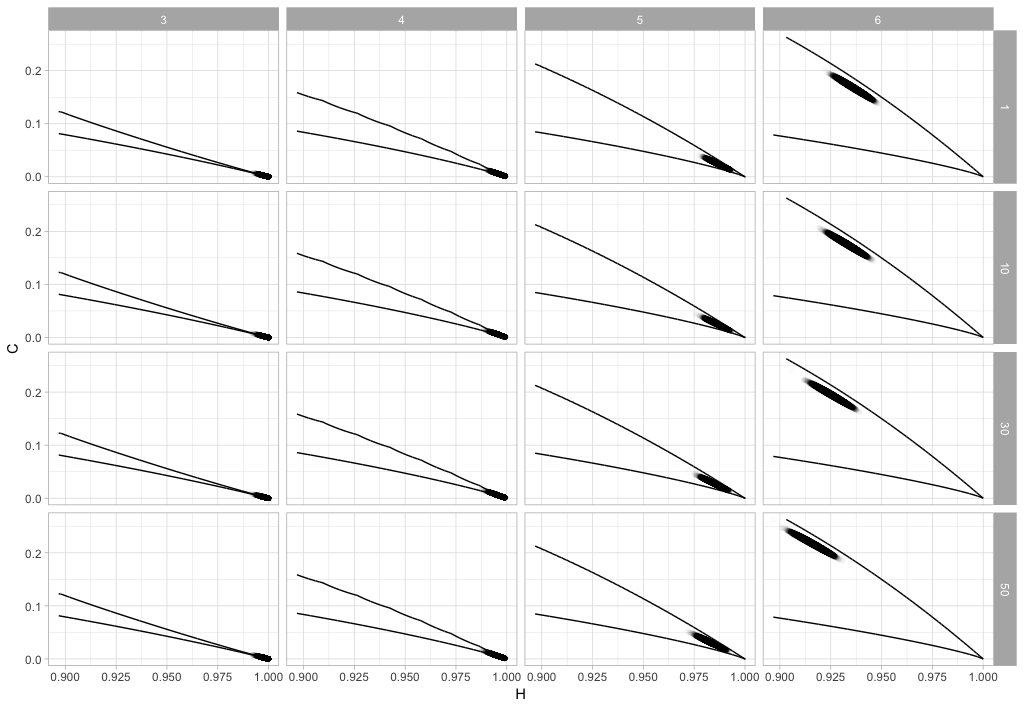
\includegraphics[width=\linewidth]{ScatterAll_Quant_1k}
	\caption{Diagramas de dispersão das sequências quânticas com $1.000$ observações para $D\in\{3, 4, 5, 6\}$ (colunas) e $\tau\in\{1, 10, 30, 50\}$ (linhas), com curvas de complexidade mínima e máxima no plano Entropia-Complexidade.}\label{Fig:ScatterAll_Quant_1k}
\end{figure}

\begin{figure}[hbt]
	\centering
	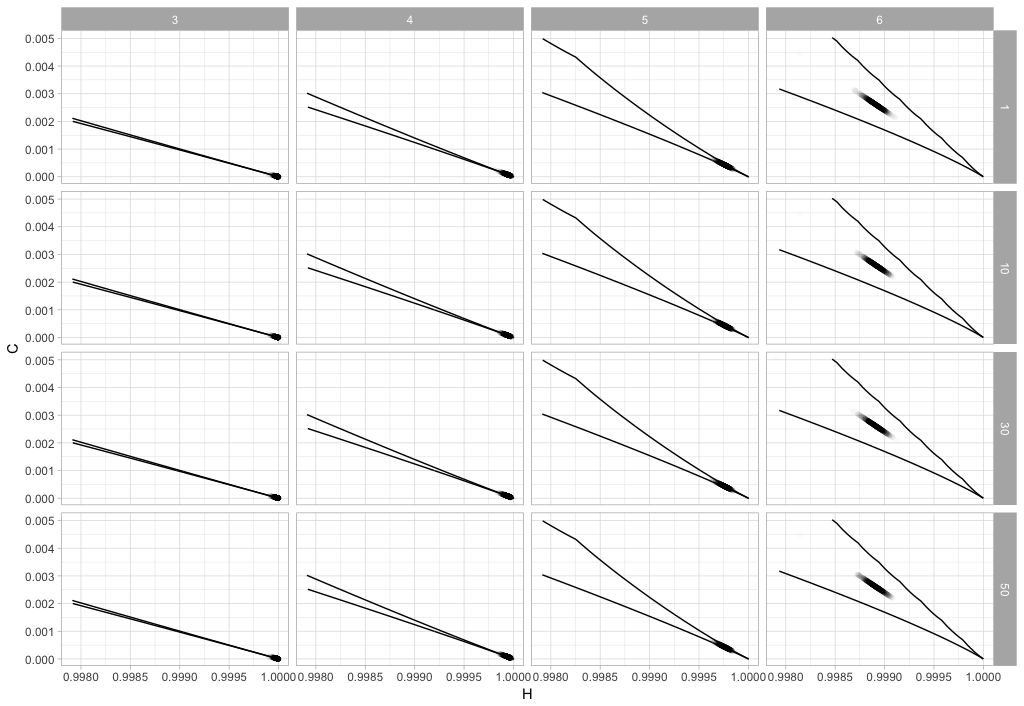
\includegraphics[width=\linewidth]{ScatterAll_Quant_50k}
	\caption{Diagramas de dispersão das sequências quânticas com $50.000$ observações para $D\in\{3, 4, 5, 6\}$ (colunas) e $\tau\in\{1, 10, 30, 50\}$ (linhas), com curvas de complexidade mínima e máxima no plano Entropia-Complexidade.}\label{Fig:ScatterAll_Quant_50k}
\end{figure}

As figuras~\ref{Fig:ScatterAll_Radio_1k} e~\ref{Fig:ScatterAll_Radio_50k} mostram os planos Entropia-Complexidade com as respectivas curvas de complexidade mínima e máxima para cada par $D\in\{3, 4, 5, 6\}$ (colunas) e $\tau\in\{1, 10, 30, 50\}$ (linhas), com os \num{52429} pontos observados a partir das sequências obtidas pelo gerador de rádio tomando $1.000$ e $50.000$ sequências respectivamente.


\begin{figure}[hbt]
	\centering
	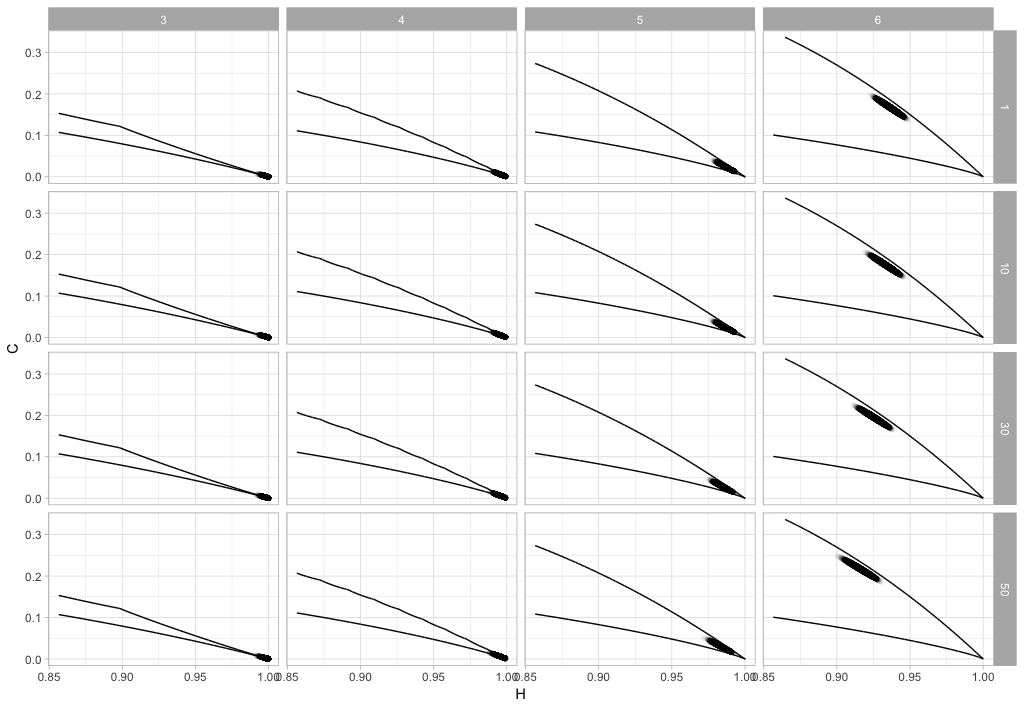
\includegraphics[width=\linewidth]{ScatterAll_Radio_1k}
	\caption{Diagramas de dispersão das sequências de rádio com $1.000$ observações para $D\in\{3, 4, 5, 6\}$ (colunas) e $\tau\in\{1, 10, 30, 50\}$ (linhas), com curvas de complexidade mínima e máxima no plano Entropia-Complexidade.}\label{Fig:ScatterAll_Radio_1k}
\end{figure}

\begin{figure}[hbt]
	\centering
	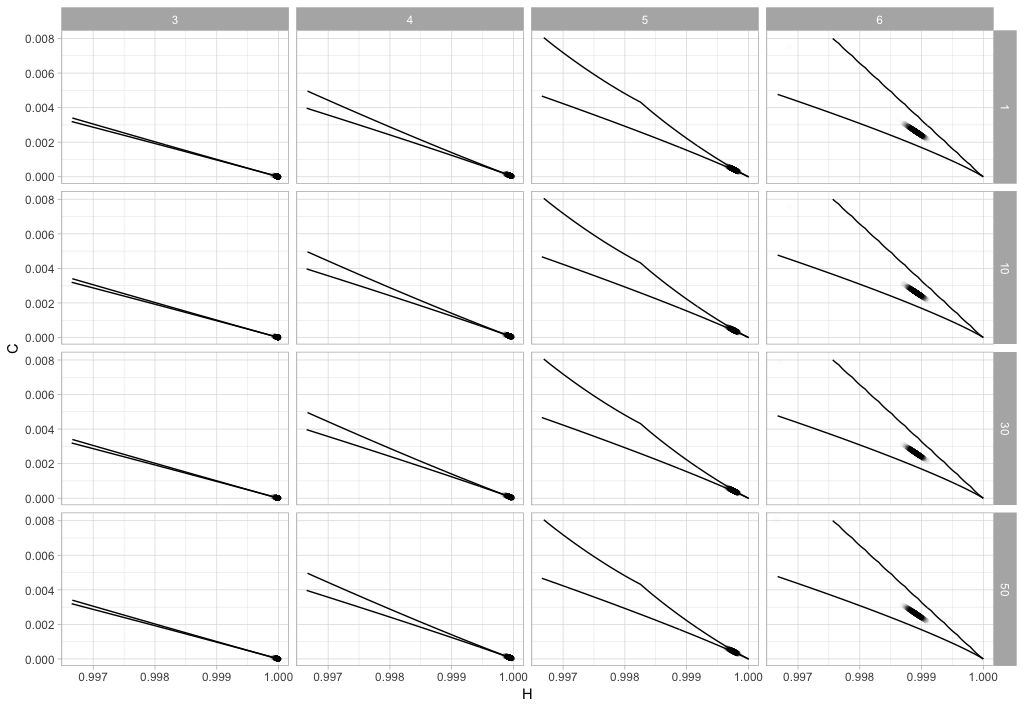
\includegraphics[width=\linewidth]{ScatterAll_Radio_50k}
	\caption{Diagramas de dispersão das sequências de rádio com $50.000$ observações para $D\in\{3, 4, 5, 6\}$ (colunas) e $\tau\in\{1, 10, 30, 50\}$ (linhas), com curvas de complexidade mínima e máxima no plano Entropia-Complexidade.}\label{Fig:ScatterAll_Radio_50k}
\end{figure}

As figuras~\ref{Fig:ScatterAll_MT_1k} e~\ref{Fig:ScatterAll_MT_50k} mostram os planos Entropia-Complexidade com as respectivas curvas de complexidade mínima e máxima para cada par $D\in\{3, 4, 5, 6\}$ (colunas) e $\tau\in\{1, 10, 30, 50\}$ (linhas), com os \num{52429} pontos observados a partir das sequências obtidas pelo gerador Mersenne-Twister tomando $1.000$ e $50.000$ sequências respectivamente.

\begin{figure}[hbt]
	\centering
	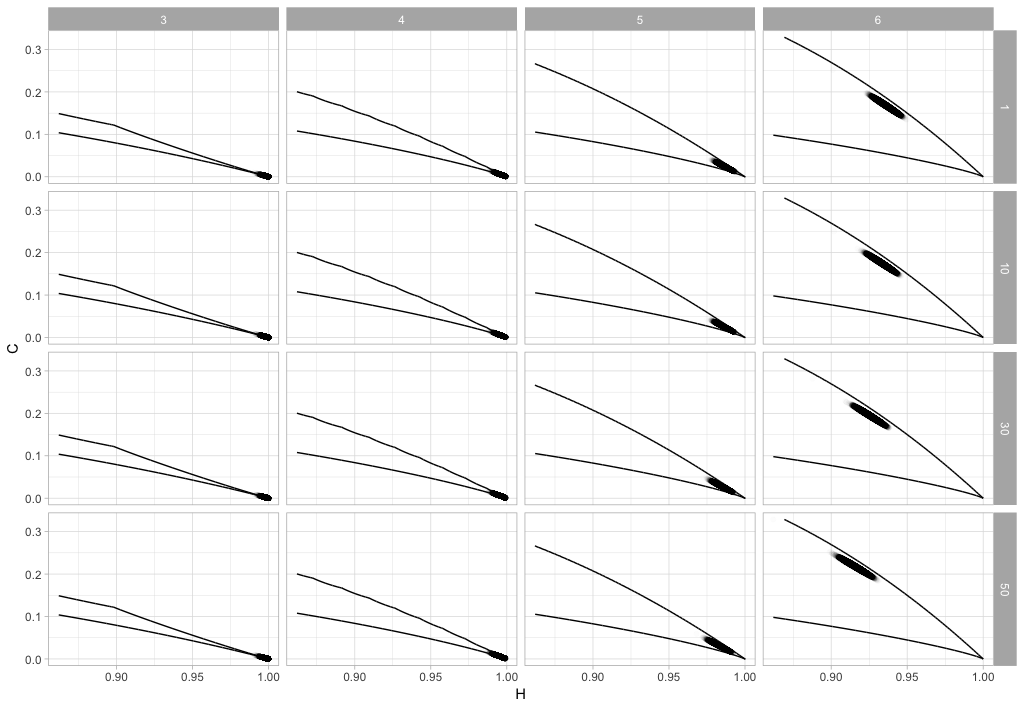
\includegraphics[width=\linewidth]{ScatterAll_MT_1k}
	\caption{Diagramas de dispersão das sequências de Mersenne-Twister com $1.000$ observações para $D\in\{3, 4, 5, 6\}$ (colunas) e $\tau\in\{1, 10, 30, 50\}$ (linhas), com curvas de complexidade mínima e máxima no plano Entropia-Complexidade.}\label{Fig:ScatterAll_MT_1k}
\end{figure}

\begin{figure}[hbt]
	\centering
	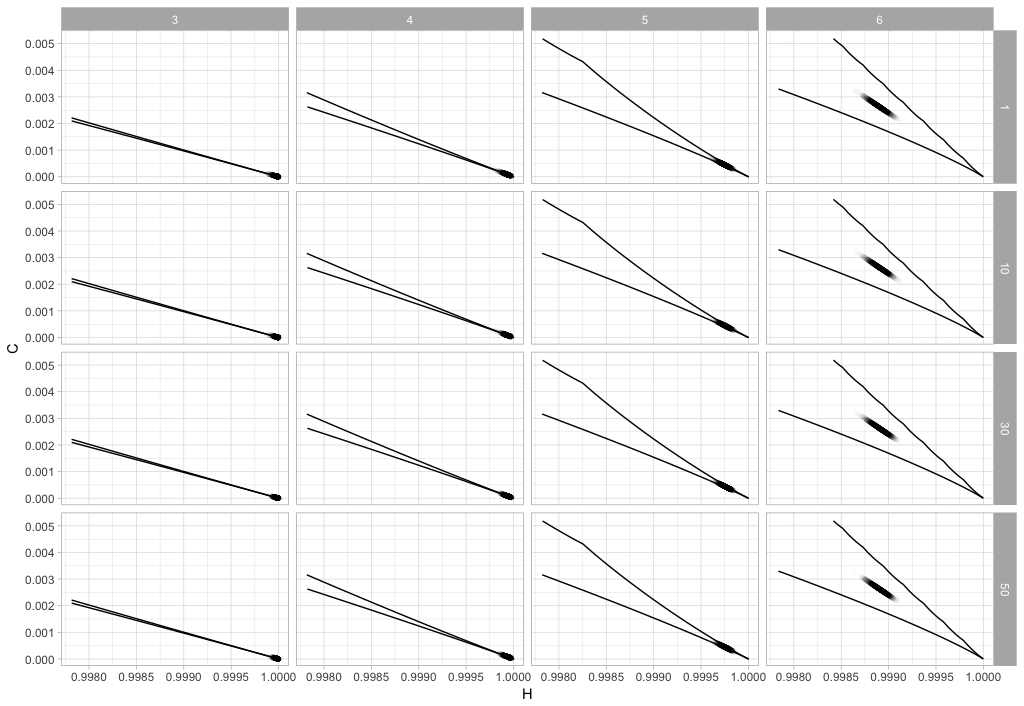
\includegraphics[width=\linewidth]{ScatterAll_MT_50k}
	\caption{Diagramas de dispersão das sequências de Mersenne-Twister com $50.000$ observações para $D\in\{3,4,5,6\}$ (colunas) e $\tau\in\{1,10,30,50\}$ (linhas), com curvas de complexidade mínima e máxima no plano Entropia-Complexidade.}\label{Fig:ScatterAll_MT_50k}
\end{figure}

A olho nu, $D$ é um fator relevante pois os diagramas de dispersão mostram comportamentos que merecem uma análise mais aprofundada, por outro lado não temos certeza de como $\tau$ e o gerador influenciam os resultados. 

As figuras~\ref{fig:GeradorIrrelevante1k} e~\ref{fig:GeradorIrrelevante50k} mostram os histogramas suavizados das distâncias para sequências de tamanho ($N=1.000$, $50.000$) respectivamente, com palavras de tamanho $D=6$  e valores de \textit{lag} ($\tau=1, 50$), sobrepondo os três geradores.
Os gráficos sugerem que o gerador é um fator irrelevante para a distribuição da distância.
Mais adiante veremos que esta impressão não se confirma totalmente.

\begin{figure} %D=6 %N 1000 t1 t 50
	\centering
		\subfigure[$D=6, \tau=1$]{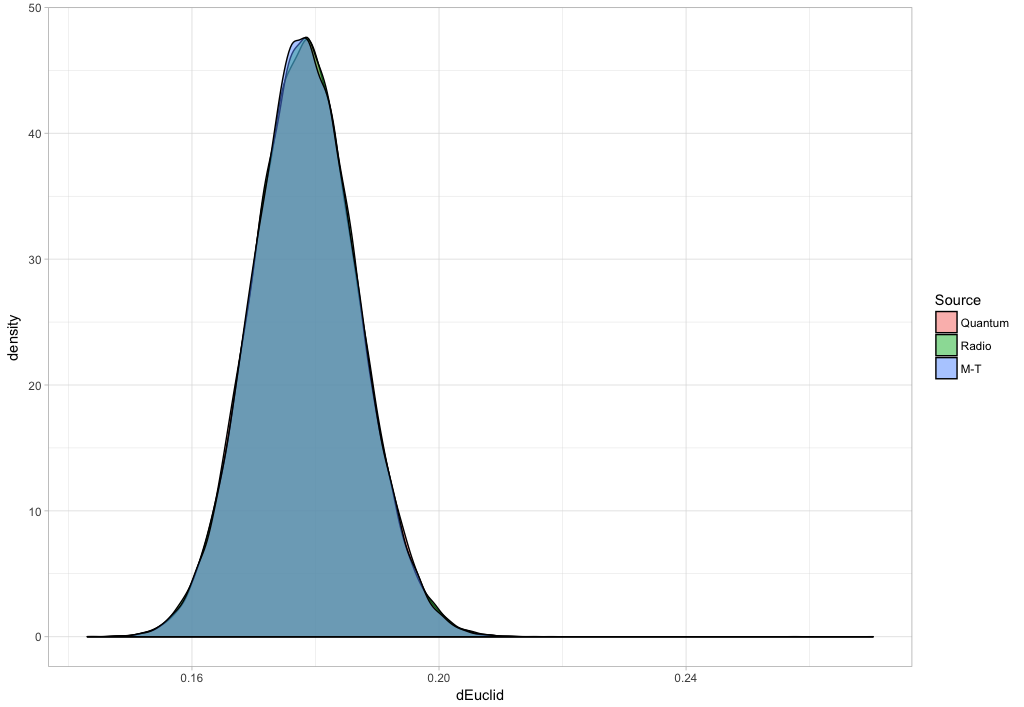
\includegraphics[width=.48\linewidth]{Hist_D6_1k_t1}}
		\subfigure[$D=6, \tau=50$]{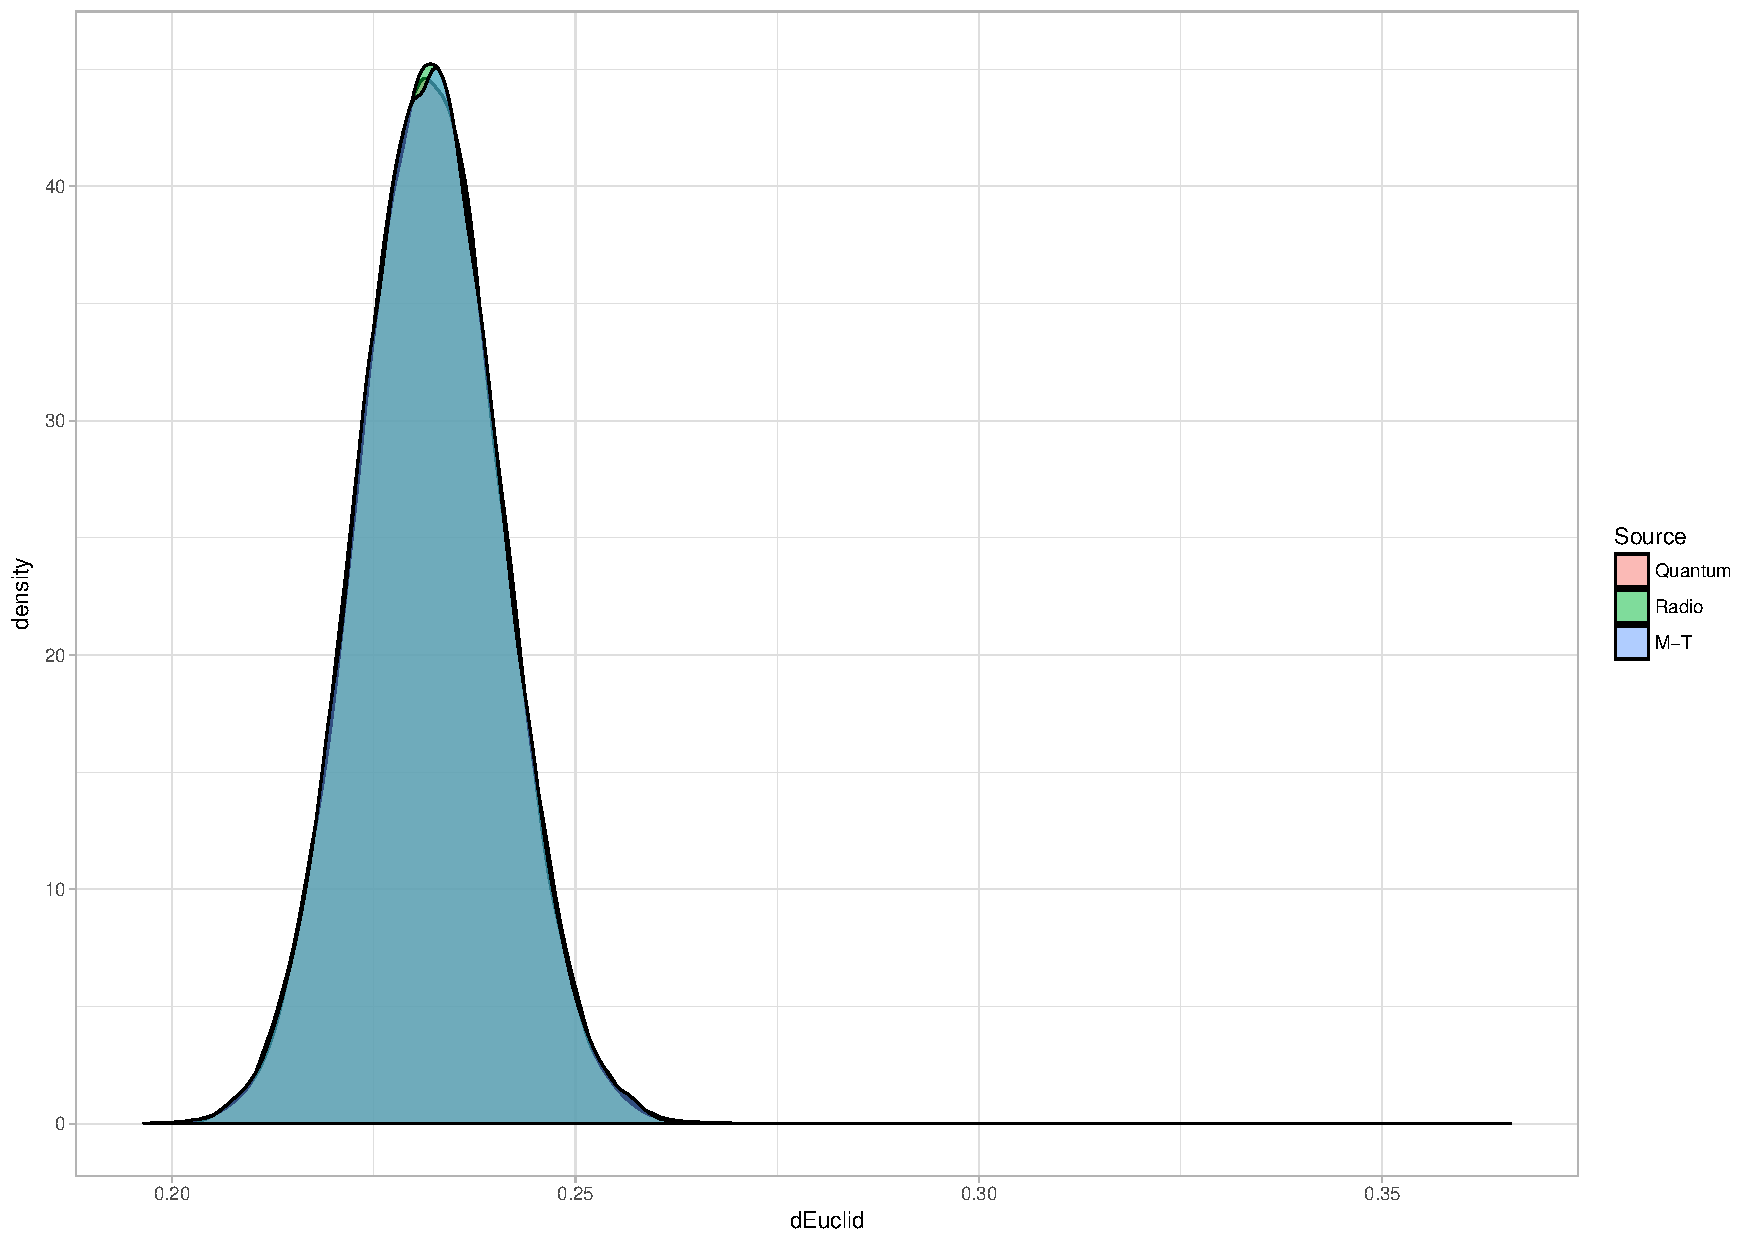
\includegraphics[width=.48\linewidth]{Hist_D6_1k_t50}}
		\caption{Histogramas suavizados de situações que sugerem que o gerador é um fator irrelevante para $N=1.000$}\label{fig:GeradorIrrelevante1k}
\end{figure}

\begin{figure} %D=6 %N 50000 t1 t 50
	\centering
		\subfigure[$D=6, \tau=1$]{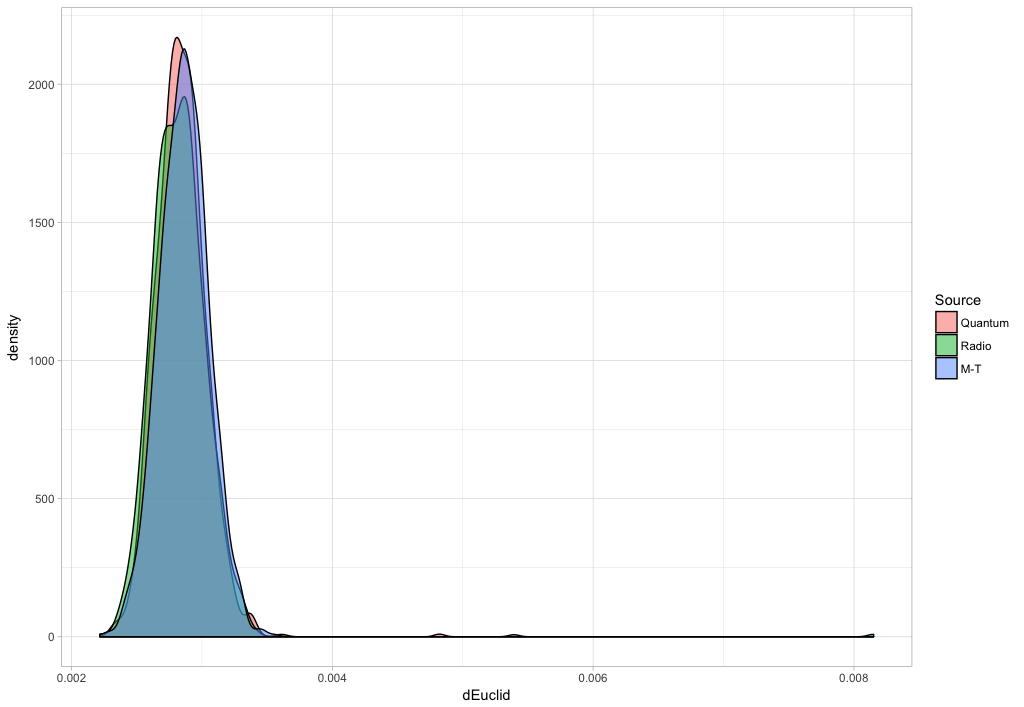
\includegraphics[width=.48\linewidth]{Hist_D6_50k_t1}}
		\subfigure[$D=6, \tau=50$]{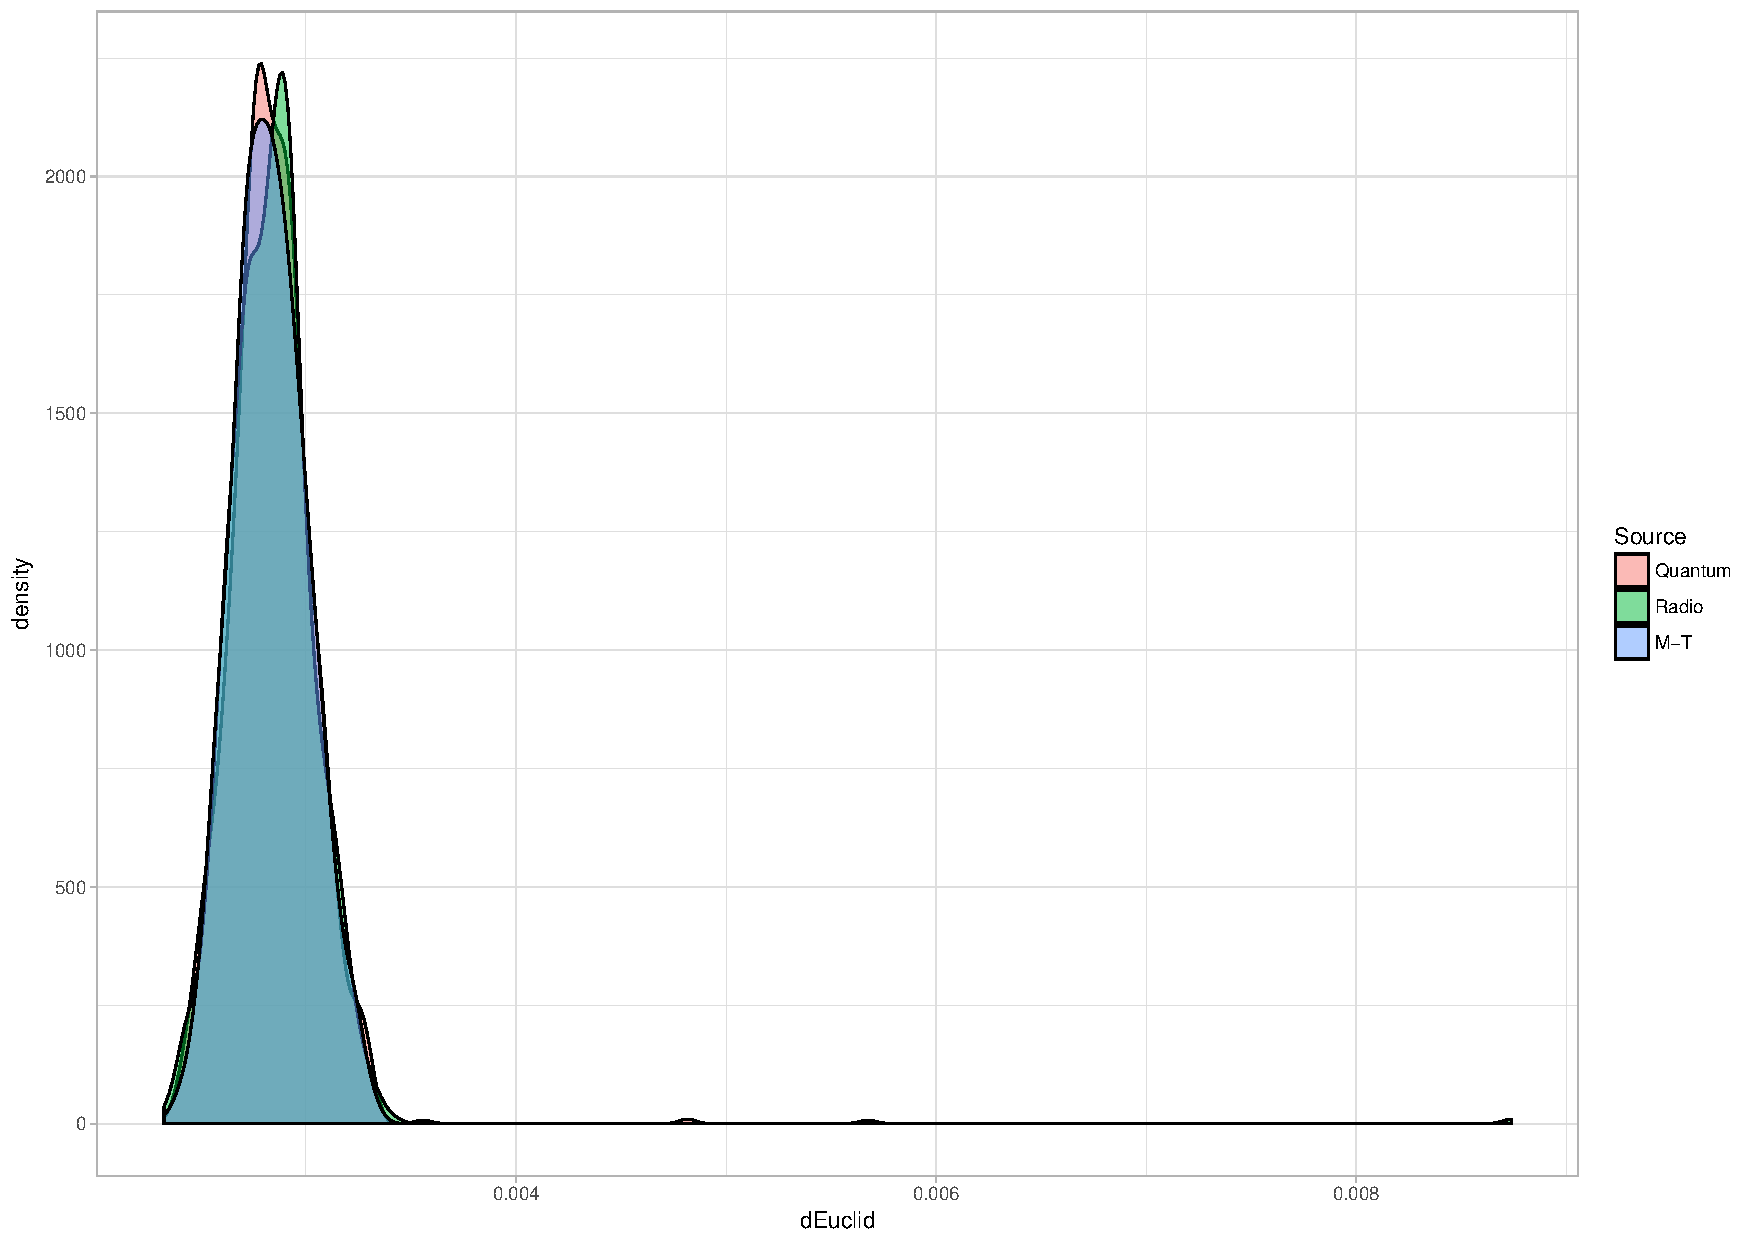
\includegraphics[width=.48\linewidth]{Hist_D6_50k_t50}}
		\caption{Histogramas suavizados de situações que sugerem que o gerador é um fator irrelevante também para $N=50.000$}\label{fig:GeradorIrrelevante50k}
\end{figure}

A figura~\ref{fig:NRelevante} mostra os histogramas suavizados das distâncias dos três geradores para palavras de tamanho $D=6$ e dois valores de \textit{lag} ($\tau=1$, $50$), sobrepondo os resultados obtidos com os dois tamanhos de sequências ($N=1.000$, $50.000$).
Os gráficos sugerem fortemente que o tamanho das sequências é um fator relevante para a distribuição da distância.

\begin{figure} %D=6 %t 1 N 1000 N 50000 (três geradores) %t 50 N 1000 N 50000 (três geradores)
	\centering
		\subfigure[$D=6$, $\tau=1$]{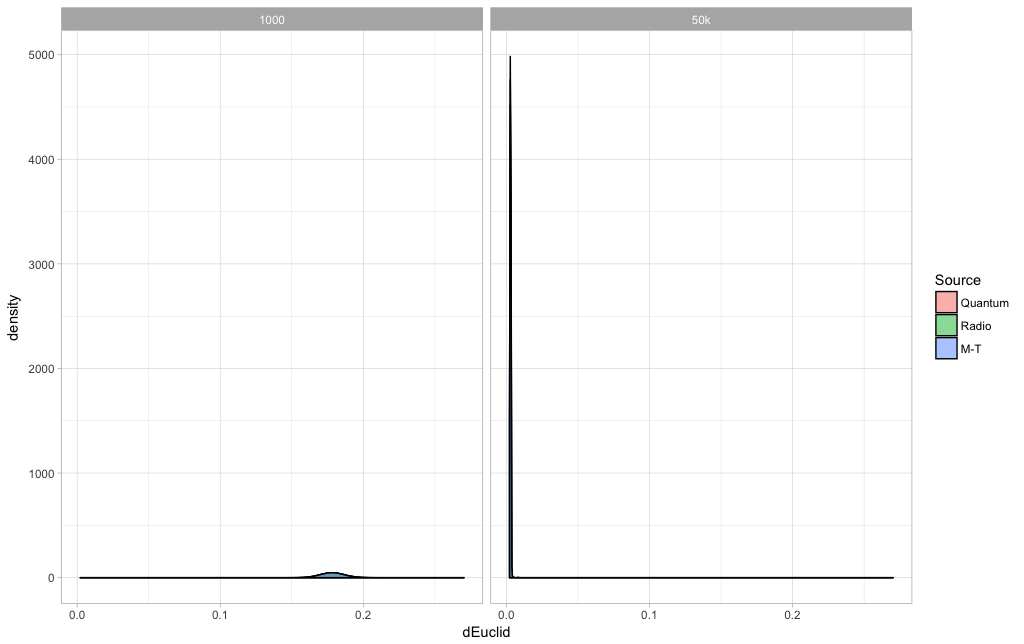
\includegraphics[width=.48\linewidth]{Hist_D6_t1}}
		\subfigure[$D=6$, $\tau=50$]{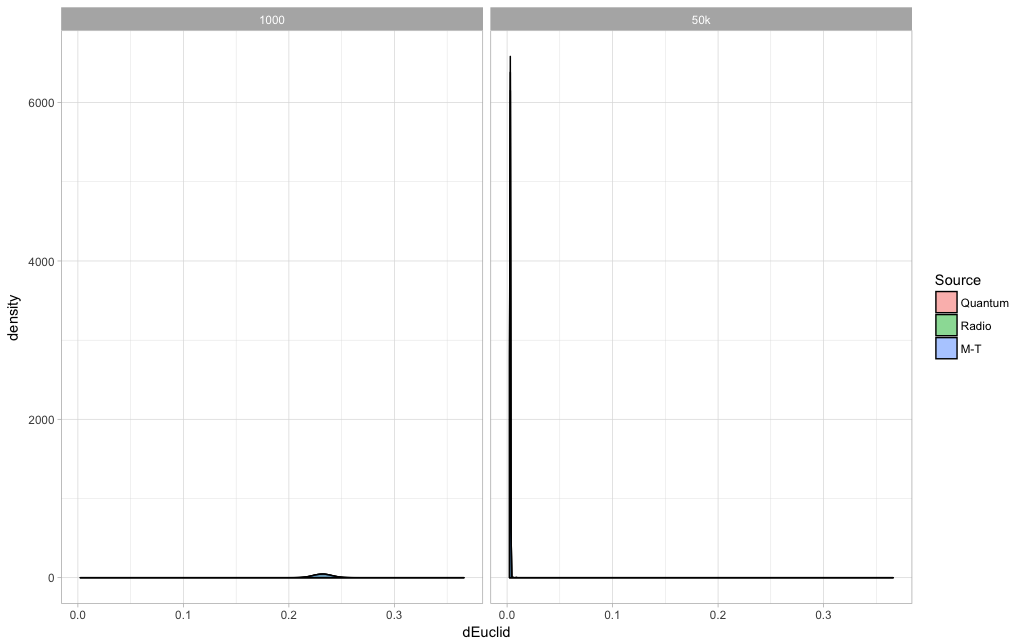
\includegraphics[width=.48\linewidth]{Hist_D6_t50}}
	\caption{Histogramas suavizados de situações que sugerem que o $N$ é um fator relevante}\label{fig:NRelevante}
\end{figure}

A figura~\ref{fig:DRelevante} mostra os histogramas suavizados das distâncias dos três geradores para dois tamanhos de sequências ($N=1.000$, $50.000$) e dois valores de \textit{lag} ($\tau=1$, $50$), sobrepondo os resultados obtidos com os diferentes tamanhos de palavras ($D=3$, $D=4$, $D=5$, $D=6$).
Os gráficos sugerem fortemente que o tamanho das palavras é um fator relevante para a distribuição da distância.

\begin{figure} %t 1 N 1000, D 3 D 4 D 5 D 6 %t 50 N 50000, D 3 D 4 D 5 D 6
	\centering
		\subfigure[$N=1.000$, $\tau=1$]{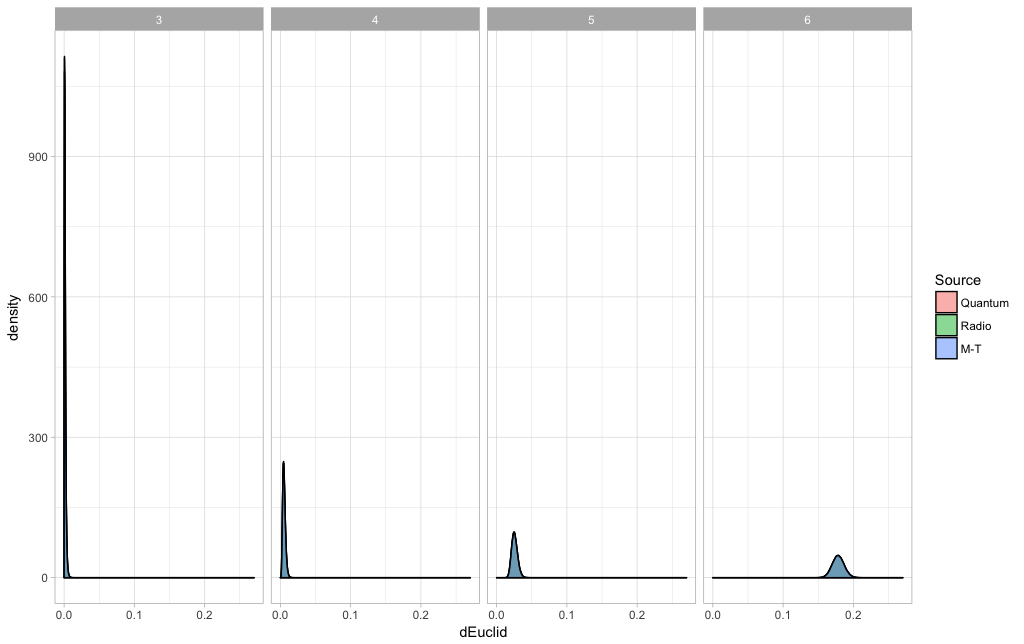
\includegraphics[width=.48\linewidth]{Hist_t1_1k}}
		\subfigure[$N=50.000$, $\tau=50$]{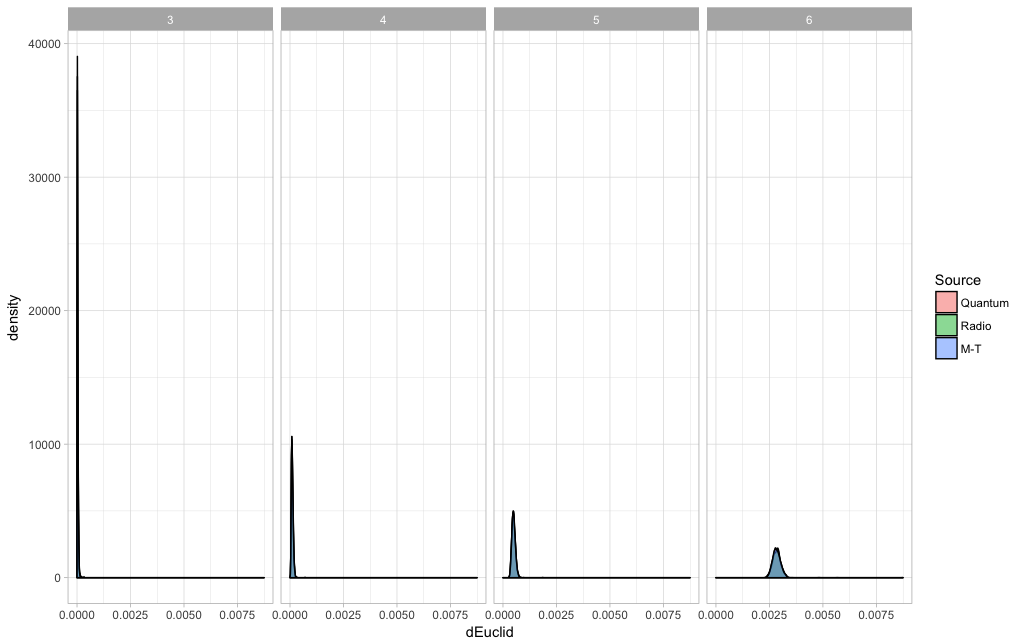
\includegraphics[width=.48\linewidth]{Hist_t50_50k}}
	\caption{Histogramas suavizados de situações que sugerem que o $D$ é um fator relevante}\label{fig:DRelevante}
\end{figure}



\begin{figure} %D 6 %N 1000, t 1 t 10 t 30 t 50 %N 50000, t 1 t 10 t 30 t 50
	\centering
	\subfigure[$N=1.000$, $D=6$]{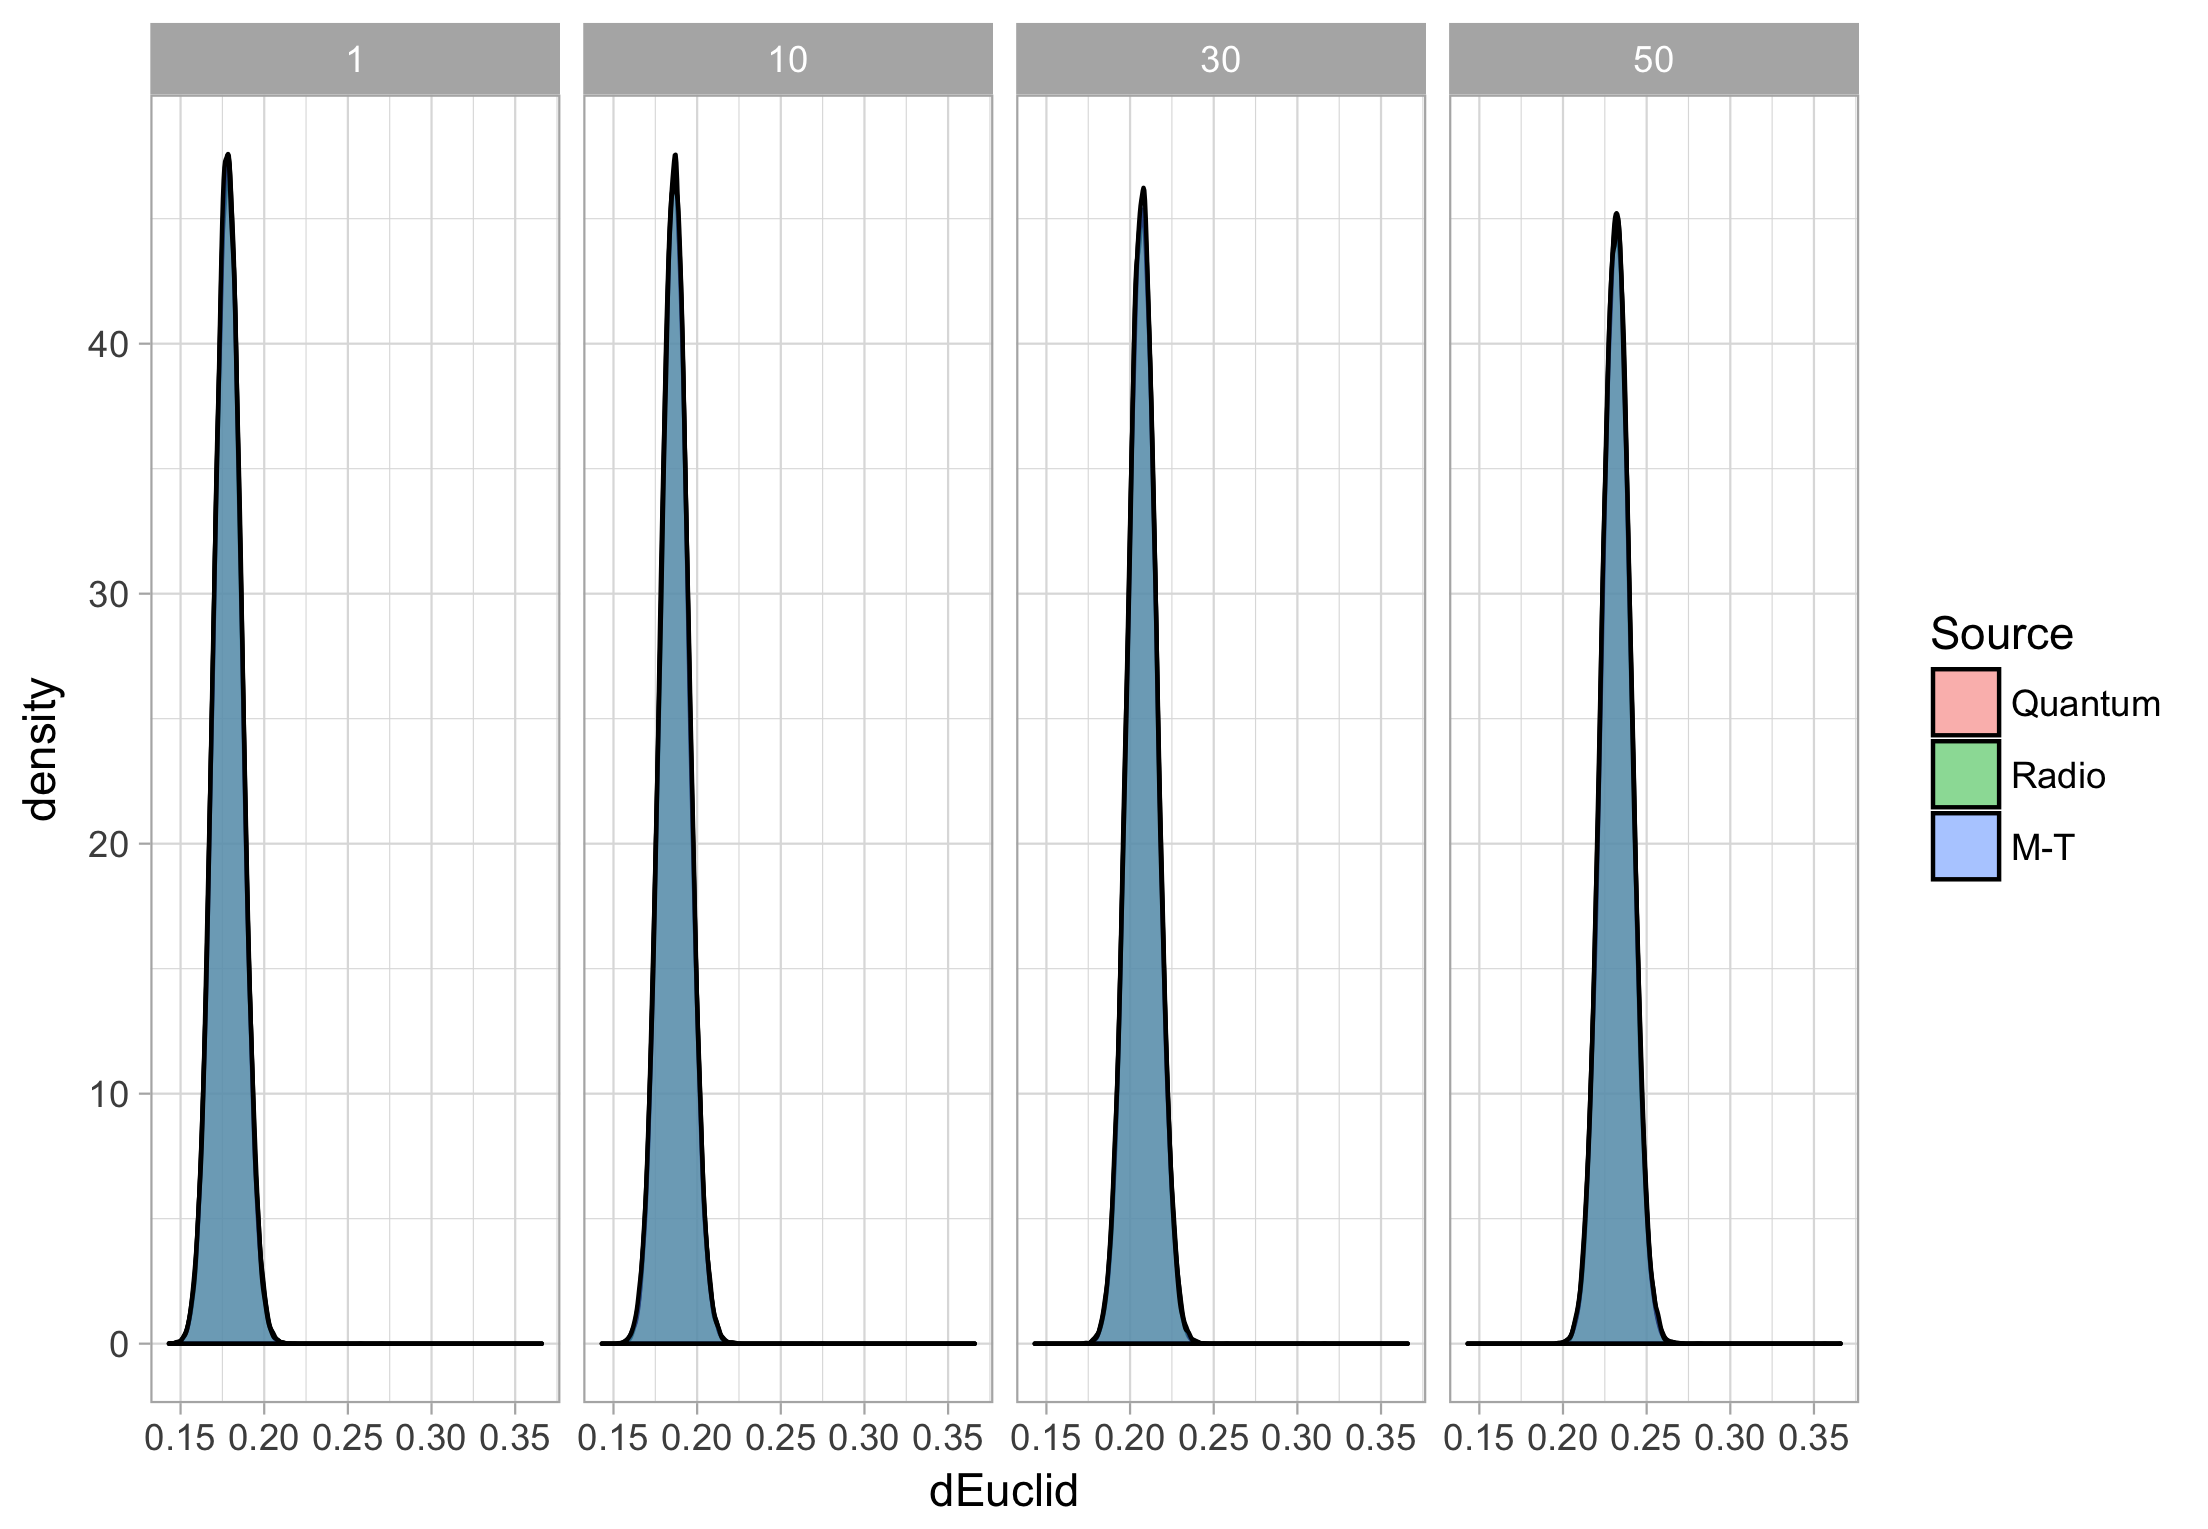
\includegraphics[width=.48\linewidth]{Hist_D6_1k}}
	\subfigure[$N=50.000$, $D=6$]{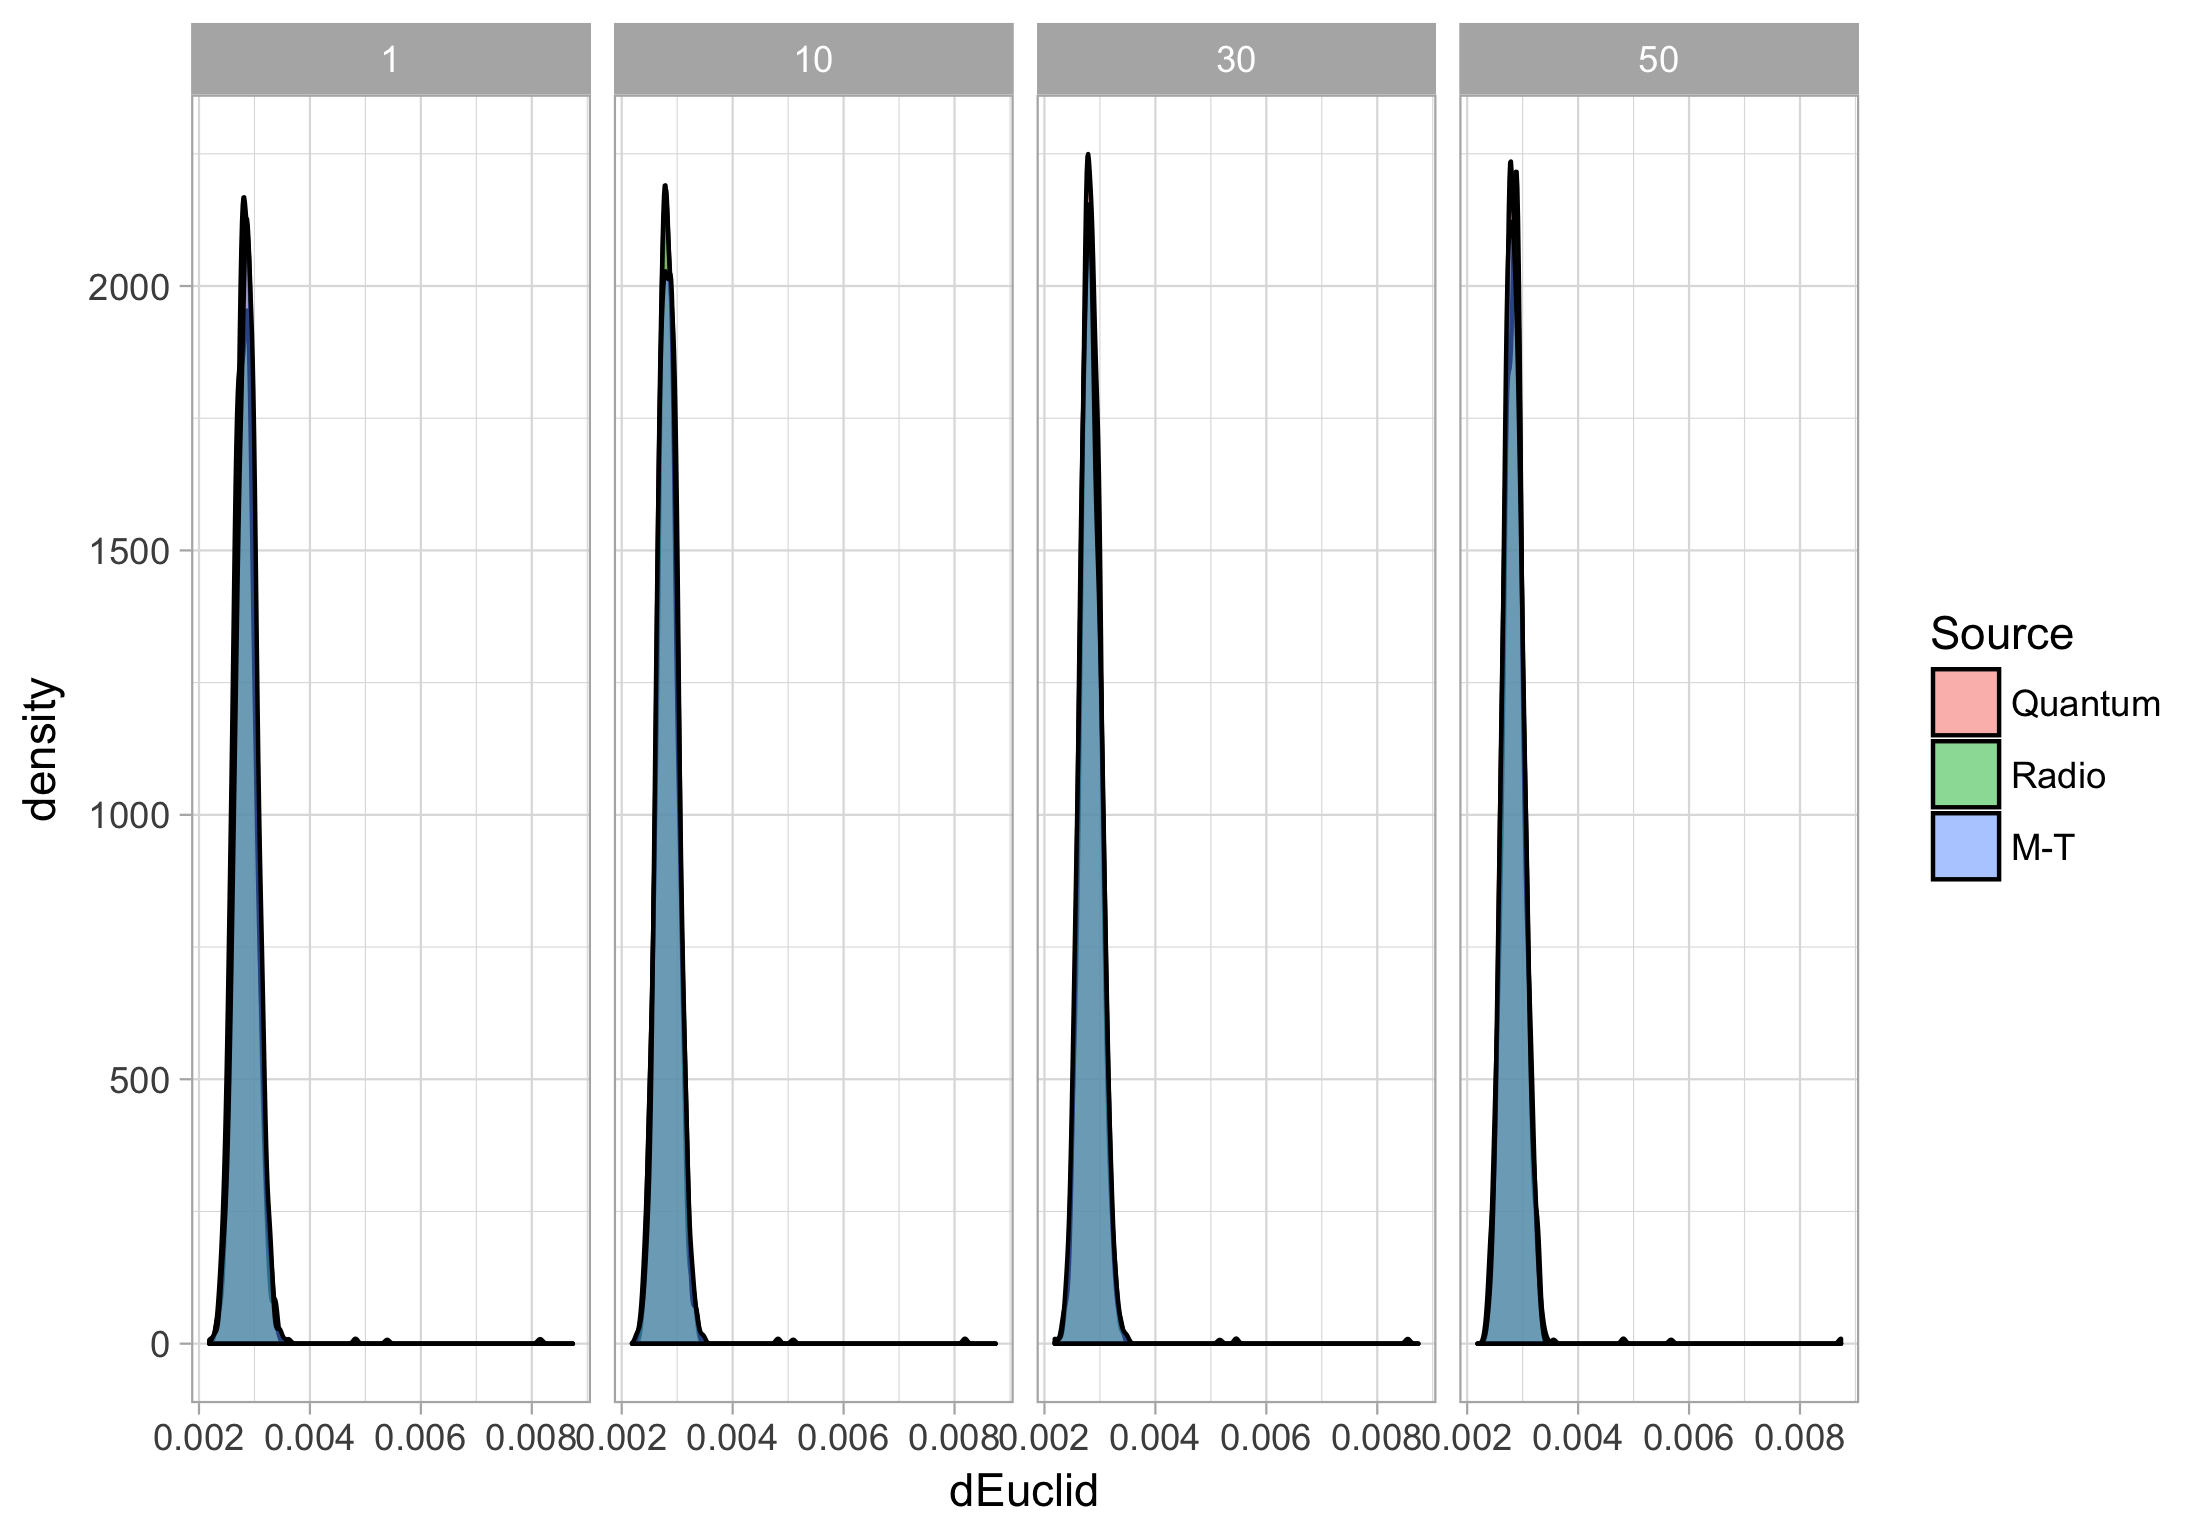
\includegraphics[width=.48\linewidth]{Hist_D6_50k}}
\caption{Histogramas suavizados de situações que sugerem que o $\tau$ é um fator relevante}\label{fig:tRelevante}
\end{figure}

Para consolidar esta análise realizamos a seguir testes Kolmogorov-Smirnov afim de analisar a influência dos fatores envolvidos nesta análise.

A Tabela~\ref{tab:KS_1000} mostra os $p$-valores dos testes de Kolmogorov-Smirnov aplicados a pares de distâncias calculadas sobre sequências de tamanho $1000$, variando $D$ e $\tau$.
Verificamos que há excelente aderência entre os pares de distâncias de sequências Quânticas e de Rádio.
Já quando a comparação é feita com distâncias de sequências de Mersenne-Twister (M-T), a aderência diminui um pouco.

\begin{table}[hbt]
	\centering
	\caption{Teste de Kolmogorov-Smirnov aplicado a pares de sequências para $1.000$ observações.}\label{tab:KS_1000}
	\begin{tabular}{cccccc}
		\toprule
		Par  &    $D$ & $\tau=1$   &   $\tau=10$   &   $\tau=30$   &   $\tau=50$   \\ \midrule
Quântica vs.\ Rádio		& $D=3$ & 0.18034676 & 0.08582490 & 0.58096350 & 0.32626542 \\
		& $D=4$ & 0.21708776 & 0.60690204 & 0.08116764 & 0.46372312  \\
		& $D=5$ & 0.32388371 & 0.53394280 & 0.46970138 & 0.02768674  \\
		& $D=6$ & 0.61501858 & 0.63403661 & 0.54795745 & 0.15353799  \\ \midrule
Quântica vs. M-T & $D=3$ & 0.09400120 & 0.22995096 & 0.36766759 &  0.03706359 \\
		& $D=4$ & 0.25188769 & 0.35844686 & 0.16768952 &  0.18237754 \\
		& $D=5$ & 0.97552039 & 0.79878301 & 0.12852918 &  0.08764347 \\
		& $D=6$ & 0.47615384 & 0.42420007 & 0.55290011 &  0.79669144 \\ \midrule
Rádio vs.\ M-T & $D=3$ & 0.008560614 & 0.496450214 & 0.982419336 & 0.390237891 \\
		& $D=4$ & 0.003804157 & 0.229503619 & 0.629158543 & 0.651783589 \\
		& $D=5$ & 0.254216237 & 0.179697451 & 0.824743440 & 0.071709252 \\
		& $D=6$ & 0.846441994 & 0.033726860 & 0.493286733 & 0.184856861 \\
		\bottomrule
	\end{tabular}
\end{table}

Os $p$-valores reportados para distâncias obtidas com sequências de tamanho $N=1000$ não permitem concluir que haja diferenças significativas.
Essa constatação será revertida ao analisar distâncias entre sequências de tamanho $N=50000$.

A Tabela~\ref{tab:KS_50k} mostra os $p$-valores dos testes de Kolmogorov-Smirnov aplicados a pares de distâncias calculadas sobre sequências de tamanho $50000$, variando $D$ e $\tau$.
Verificamos que há excelente aderência entre os pares de distâncias de sequências Quânticas e de Rádio.
Já quando a comparação é feita com distâncias de sequências de Mersenne-Twister (M-T), a aderência diminui de forma sistemática e significativa para $\tau=1$.

\begin{table}[hbt]
	\centering
	\caption{Teste de Kolmogorov-Smirnov aplicado a pares de sequências para $50.000$ observações.}\label{tab:KS_50k}
	\begin{tabular}{cccccc}
		\toprule
		Par  & $D$ &   $\tau=1$   &   $\tau=10$   &   $\tau=30$   &   $\tau=50$   \\ \midrule
Quântica vs.\ Rádio		& $D=3$ & 0.13862662 & 0.93677447 & 0.07714702 &  0.46405291 \\
		& $D=4$ & 0.68079537 & 0.90035466 & 0.60801914 &  0.77908261 \\
		& $D=5$ & 0.14371256 & 0.76662067 & 0.64456996 &  0.91315843 \\
		& $D=6$ & 0.02268670 & 0.49307044 & 0.53135926 &  0.30074267 \\ \midrule
Quântica vs.\ M-T & $D=3$ & 6.074571e-10 & 1.388898e-01 & 2.682058e-01 & 4.822849e-01 \\
		& $D=4$ & 6.592620e-09 & 2.987721e-02 & 8.438134e-01 & 7.923220e-01 \\
		& $D=5$ & 9.424114e-08 & 3.289299e-02 & 7.681676e-01 & 8.405168e-01 \\
		& $D=6$ & 9.058821e-04 & 7.075225e-01 & 2.982731e-01 & 3.614763e-01 \\ \midrule
Rádio vs.\ M-T		& $D=3$ & 1.226271e-09 & 1.609665e-01 & 1.465970e-01 & 1.914937e-01 \\
		& $D=4$ & 2.190462e-10 & 1.277762e-02 & 2.069821e-01 & 9.963221e-01 \\
		& $D=5$ & 1.438372e-11 & 1.267622e-02 & 4.364935e-01 & 9.999998e-01 \\
		& $D=6$ & 3.749001e-06 & 2.263466e-01 & 7.419248e-01 & 4.014641e-01 \\
		\bottomrule
	\end{tabular}
\end{table}

Os $p$-valores observados na Tabela~\ref{tab:KS_50k} nos levam a concluir que não é possível desconsiderar a fonte de dados como um fator relevante quando se trata do gerador de Mersenne-Twister.
Já as distâncias das sequências produzidas pelos geradores Quântico e de Rádio são indistinguíveis e, portanto, não podemos descartar a hipótese dessas fontes serem idênticas para a medida considerada.

%A figura~\ref{Fig:ScatterAllRandom} mostra os planos Entropia-Complexidade com as respectivas curvas de complexidade mínima e máxima para cada par $D\in\{3,4,5,6\}$ (colunas) e $\tau\in\{1,10,30,50\}$ (linhas), com os \num{52429} pontos observados a partir das sequências obtidas pelo gerador de rádio.
%Os pontos foram desenhados com \SI{1}{\percent} de transparência, para evidenciar as regiões mais e menos densas.
%
%\begin{figure}[hbt]
%	\centering
%	\includegraphics[width=\linewidth]{ScatterAllRandom}
%	\caption{Diagramas de dispersão das sequências de rádio para $D\in\{3,4,5,6\}$ (colunas) e $\tau\in\{1,10,30,50\}$ (linhas), com curvas de complexidade mínima e máxima no plano Entropia-Complexidade.}\label{Fig:ScatterAllRandom}
%\end{figure}
%
%A figura~\ref{Fig:ScatterAllMT} mostra os planos Entropia-Complexidade com as respectivas curvas de complexidade mínima e máxima para cada par $D\in\{3,4,5,6\}$ (colunas) e $\tau\in\{1,10,30,50\}$ (linhas), com os \num{52429} pontos observados a partir das sequências obtidas pelo gerador de Mersenne-Twister.
%Os pontos foram desenhados com \SI{1}{\percent} de transparência, para evidenciar as regiões mais e menos densas.
%
%\begin{figure}[hbt]
%	\centering
%	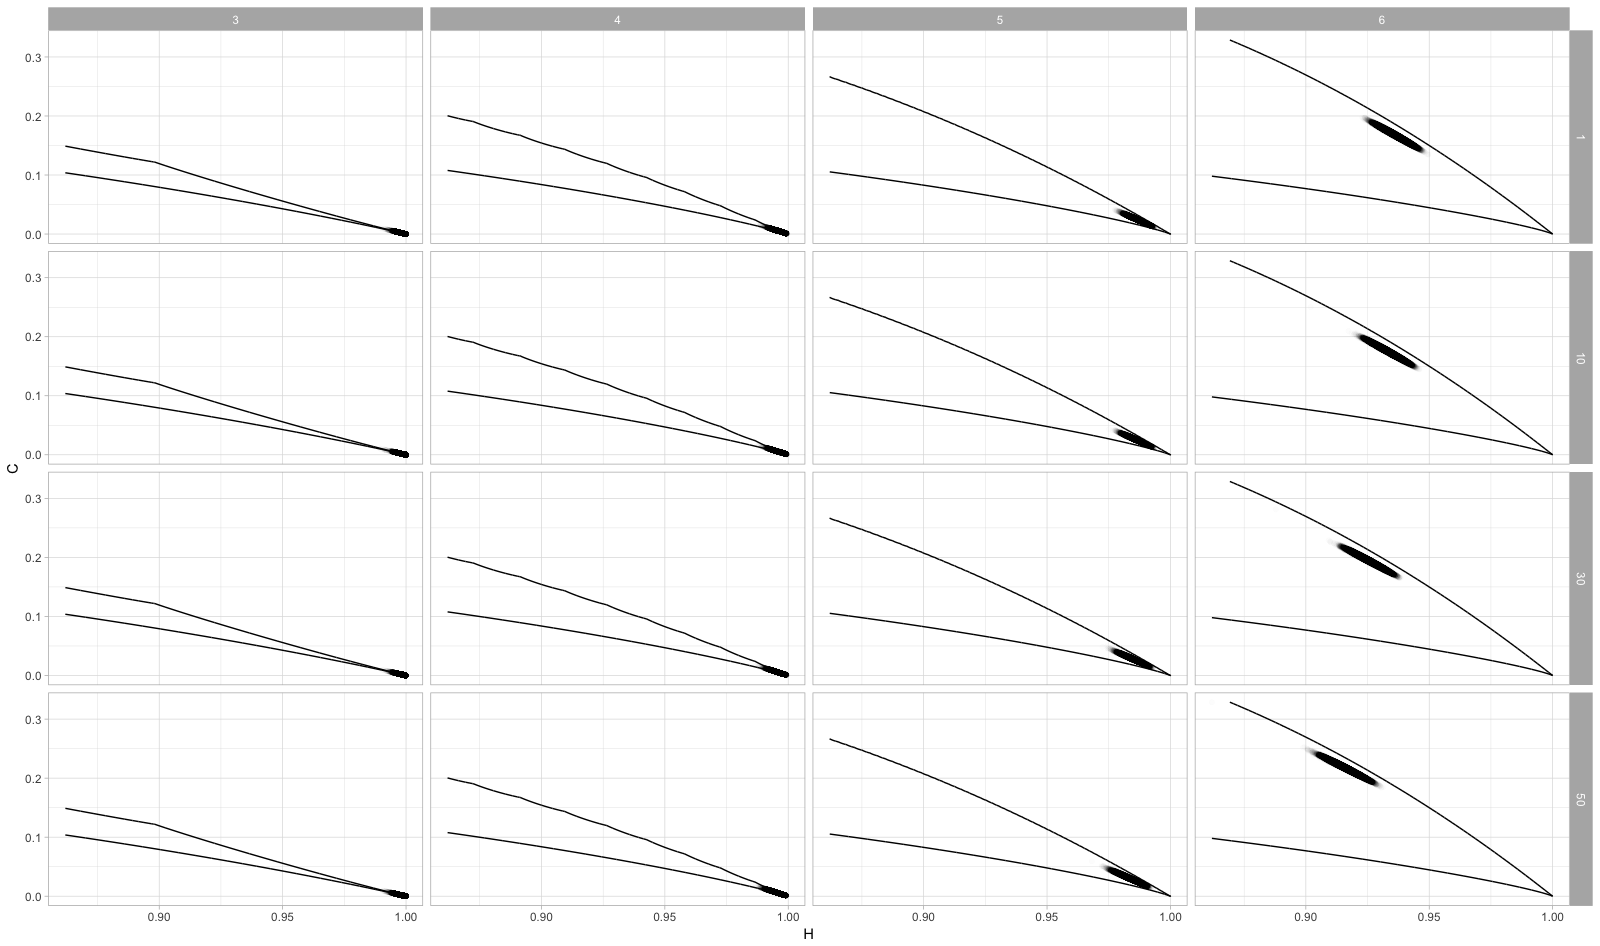
\includegraphics[width=\linewidth]{ScatterAllMT}
%	\caption{Diagramas de dispersão das sequências de Mersenne-Twister para $D\in\{3,4,5,6\}$ (colunas) e $\tau\in\{1,10,30,50\}$ (linhas), com curvas de complexidade mínima e máxima no plano Entropia-Complexidade.}\label{Fig:ScatterAllMT}
%\end{figure}

\begin{figure}[hbt]
\centering
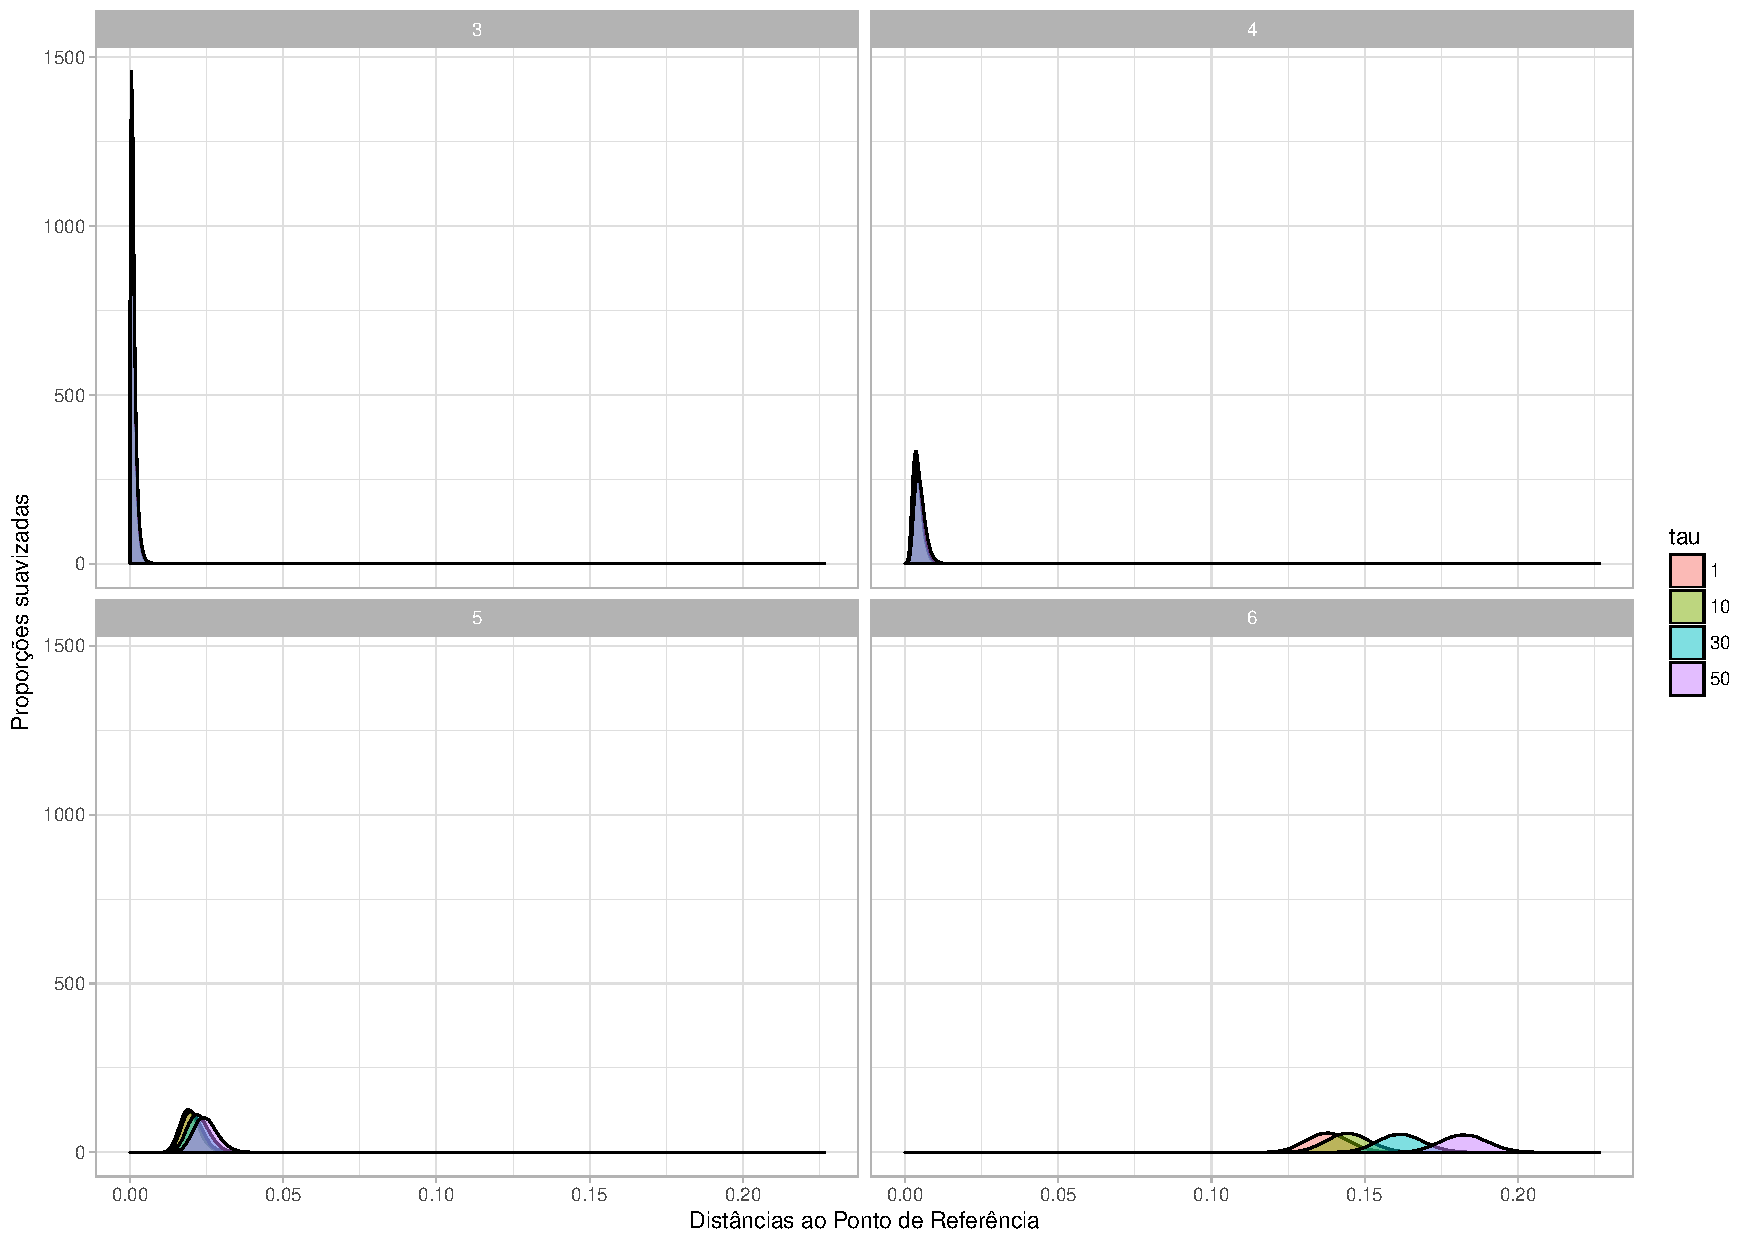
\includegraphics[width=\linewidth]{HistoDistanciasQuantTodas}
\caption{Histogramas suavizados das distâncias euclidianas dos padrões ao ponto de referência, para $D\in\{3,4,5,6\}$ (colunas) e $\tau\in\{1,10,30,50\}$ (linhas).}\label{Fig:HistoDistanciasQuantTodas}
\end{figure}

A figura~\ref{Fig:HistoDistanciasQuantTodas} sugere que o comportamento das distâncias euclidianas ao ponto de referência muda conforme o tamanho do padrão $D$ varia.
Além disso, também são perceptíveis mudanças de comportamento em função do \textit{lag} $\tau$ quando $D=5,6$.

%A figura~\ref{Fig:HistoDistanciasRandTodas} sugere que o comportamento das distâncias euclidianas ao ponto de referência muda conforme o tamanho do padrão $D$ varia.
%Além disso, também são perceptíveis mudanças de comportamento em funçao do \textit{lag} $\tau$ quando $D=5,6$.


%\begin{figure}[hbt]
%	\centering
%	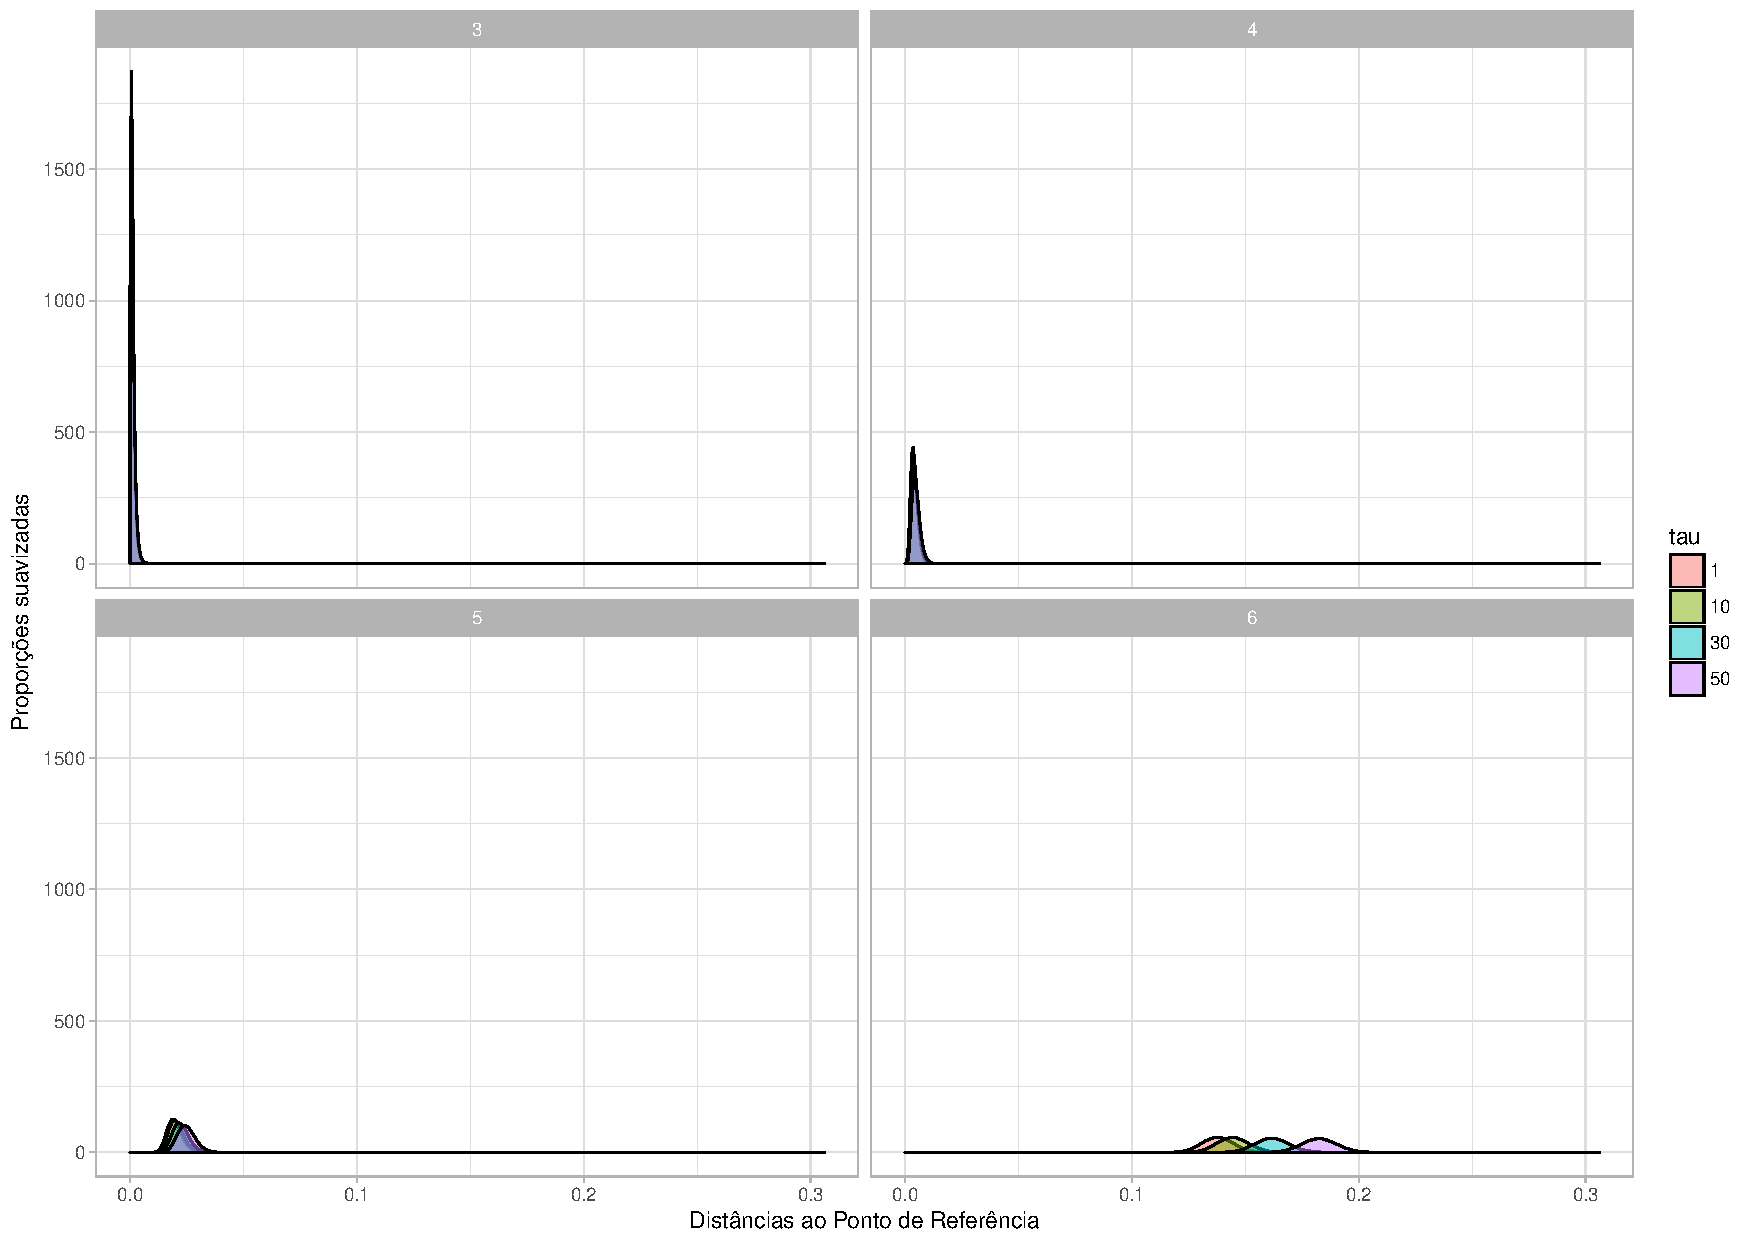
\includegraphics[width=\linewidth]{HistoDistanciasRandTodas}
%	\caption{Histogramas suavizados das distâncias euclidianas dos padrões ao ponto de referência, para $D\in\{3,4,5,6\}$ (colunas) e $\tau\in\{1,10,30,50\}$ (linhas).}\label{Fig:HistoDistanciasRandTodas}
%\end{figure}

Da análise aqui apresentada concluímos que, à luz da distância do ponto característico de uma sequência ao ponto de referência, os dois geradores físicos produzem sequências indistinguíveis.
Diante disso, nos cálculos subsequentes faremos a junção desses conjuntos de dados, que denominaremos simplesmente ``aleatórios'' no que segue.

Já o gerador de Mersenne-Twister apresenta diferenças em relação aos geradores de origem física.
Por se tratar de um gerador algorítmico e, portanto, pseudoaleatório, ele será tratado como objeto de análise e não como padrão para estabelecer critérios de qualidade.

No que segue analisaremos o comportamento dessas distâncias em detalhes.

\section{Análise das regiões de confiança}

Feita a junção das distâncias dos pontos característicos ao ponto de referência das sequências produzidas pelos geradores quântico e de rádio (sequências aleatórias), 
para cada situação de $N=1.000, 50.000$, $D=3, 4, 5, 6$ e $\tau=1, 10, 30, 50$, o próximo passo consiste em calcular os quantis relevantes.

Inicialmente ilustraremos apenas duas situações.
A figura~\ref{Fig:AleattD3tau1} mostra os padrões das sequências aleatórias para o caso $N=1.000$, $D=3$ e $\tau=1$ no plano Entropia-Complexidade, junto com os quantis de \SI{90}{\percent}, \SI{95}{\percent}, \SI{99}{\percent} e \SI{99,9}{\percent} em escala linear (figura~\ref{Fig:scatter1000D3t1}) e em escala logarítmica (figura~\ref{Fig:scatter1000D3t1_log}).

\begin{figure}
\centering
\subfigure[Escala linear\label{Fig:scatter1000D3t1}]{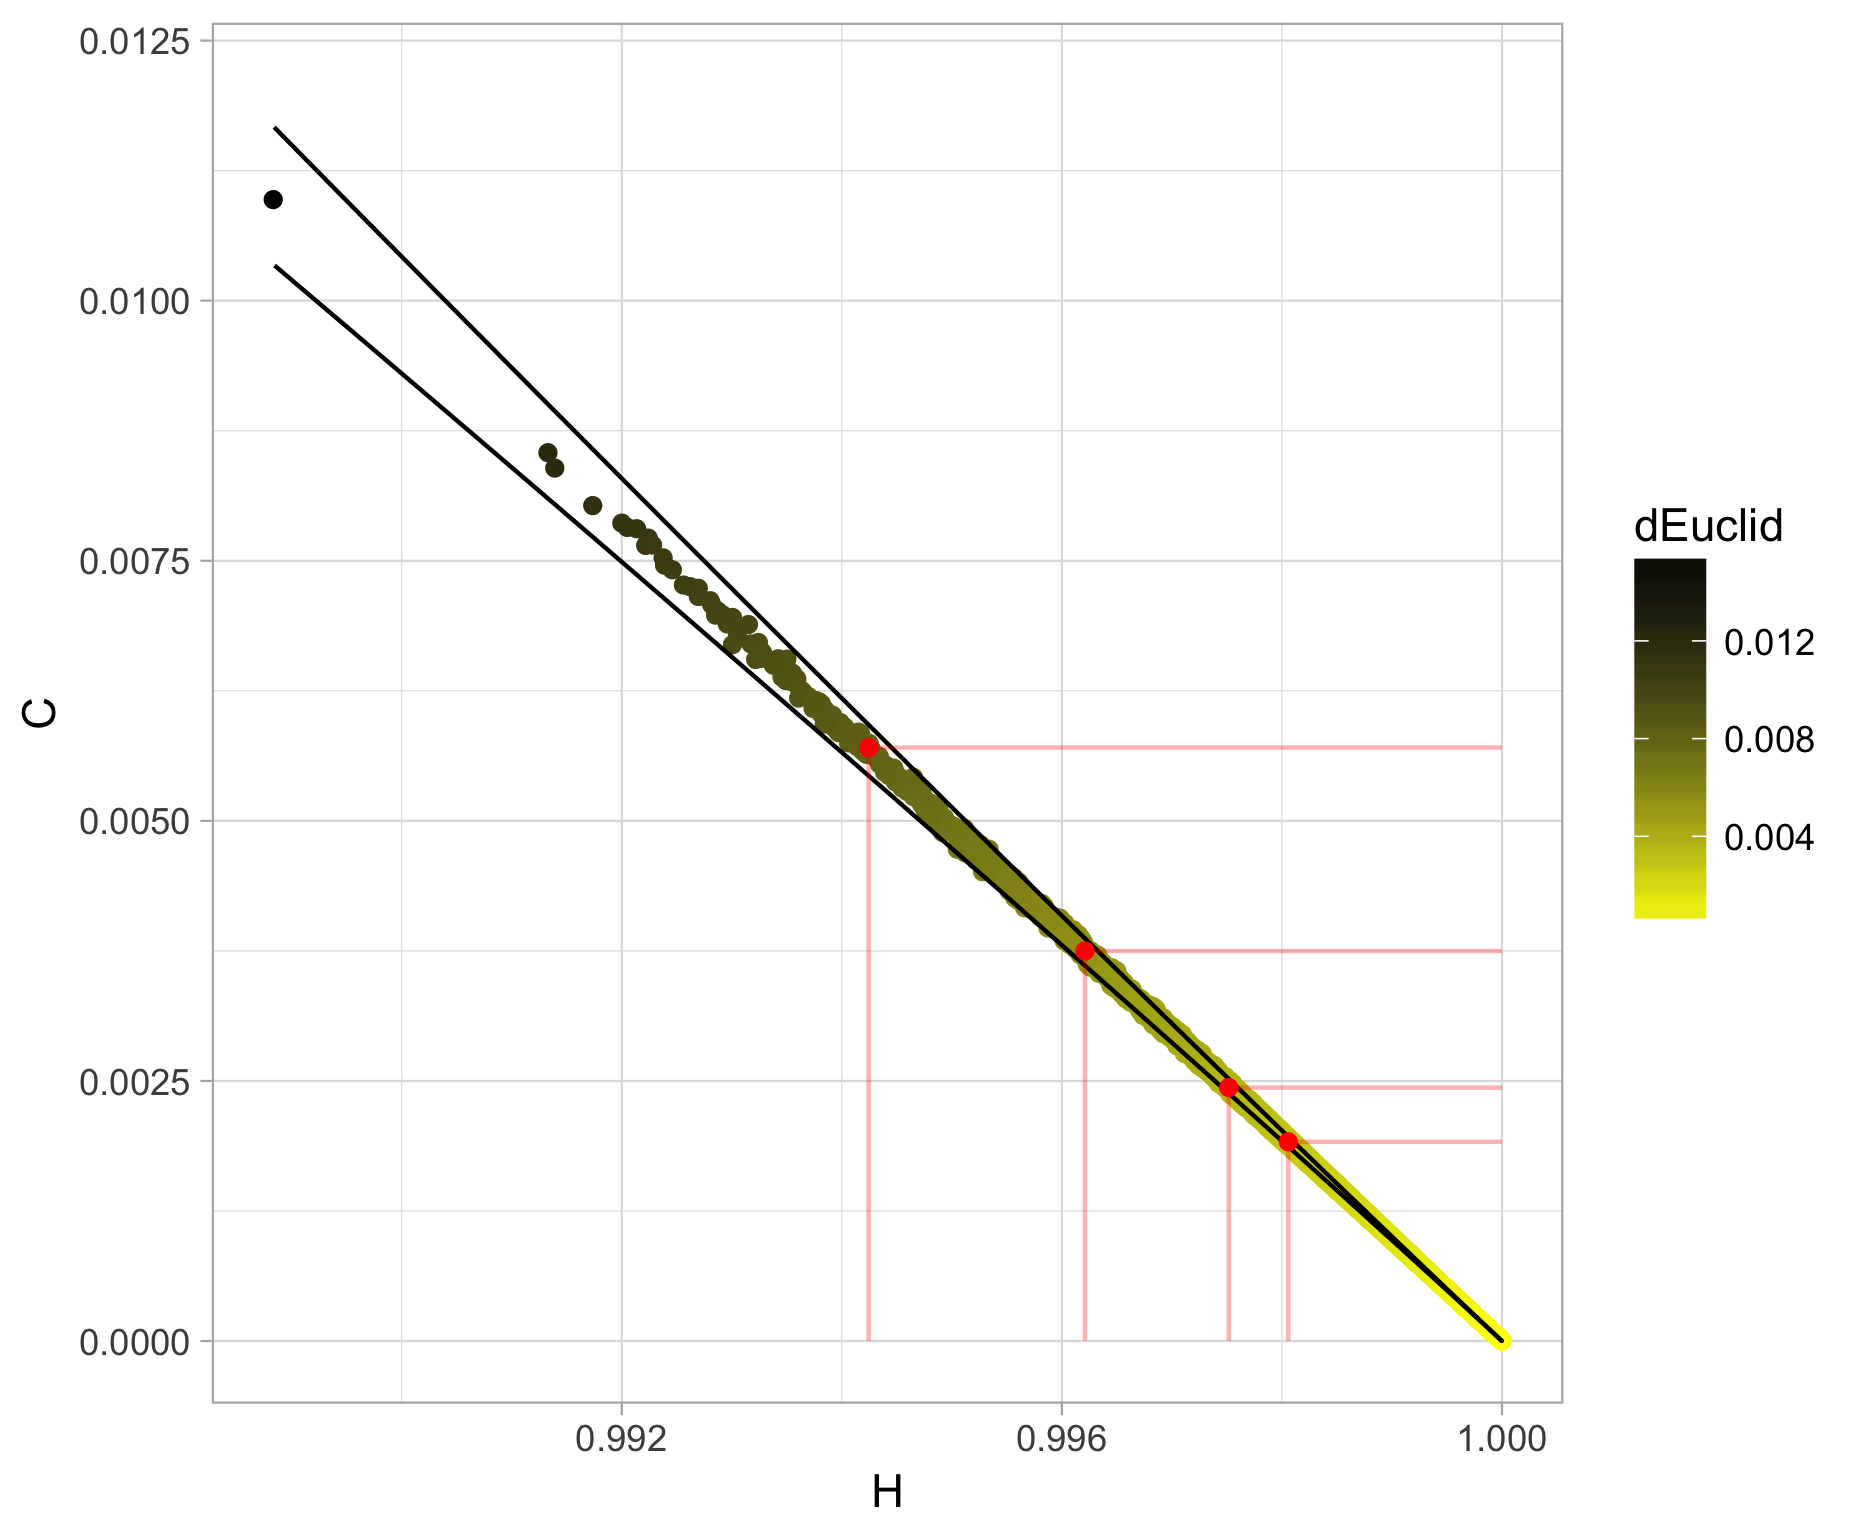
\includegraphics[width=.48\linewidth]{scatter1000D3t1}}
\subfigure[Escala logarítmica\label{Fig:scatter1000D3t1_log}]{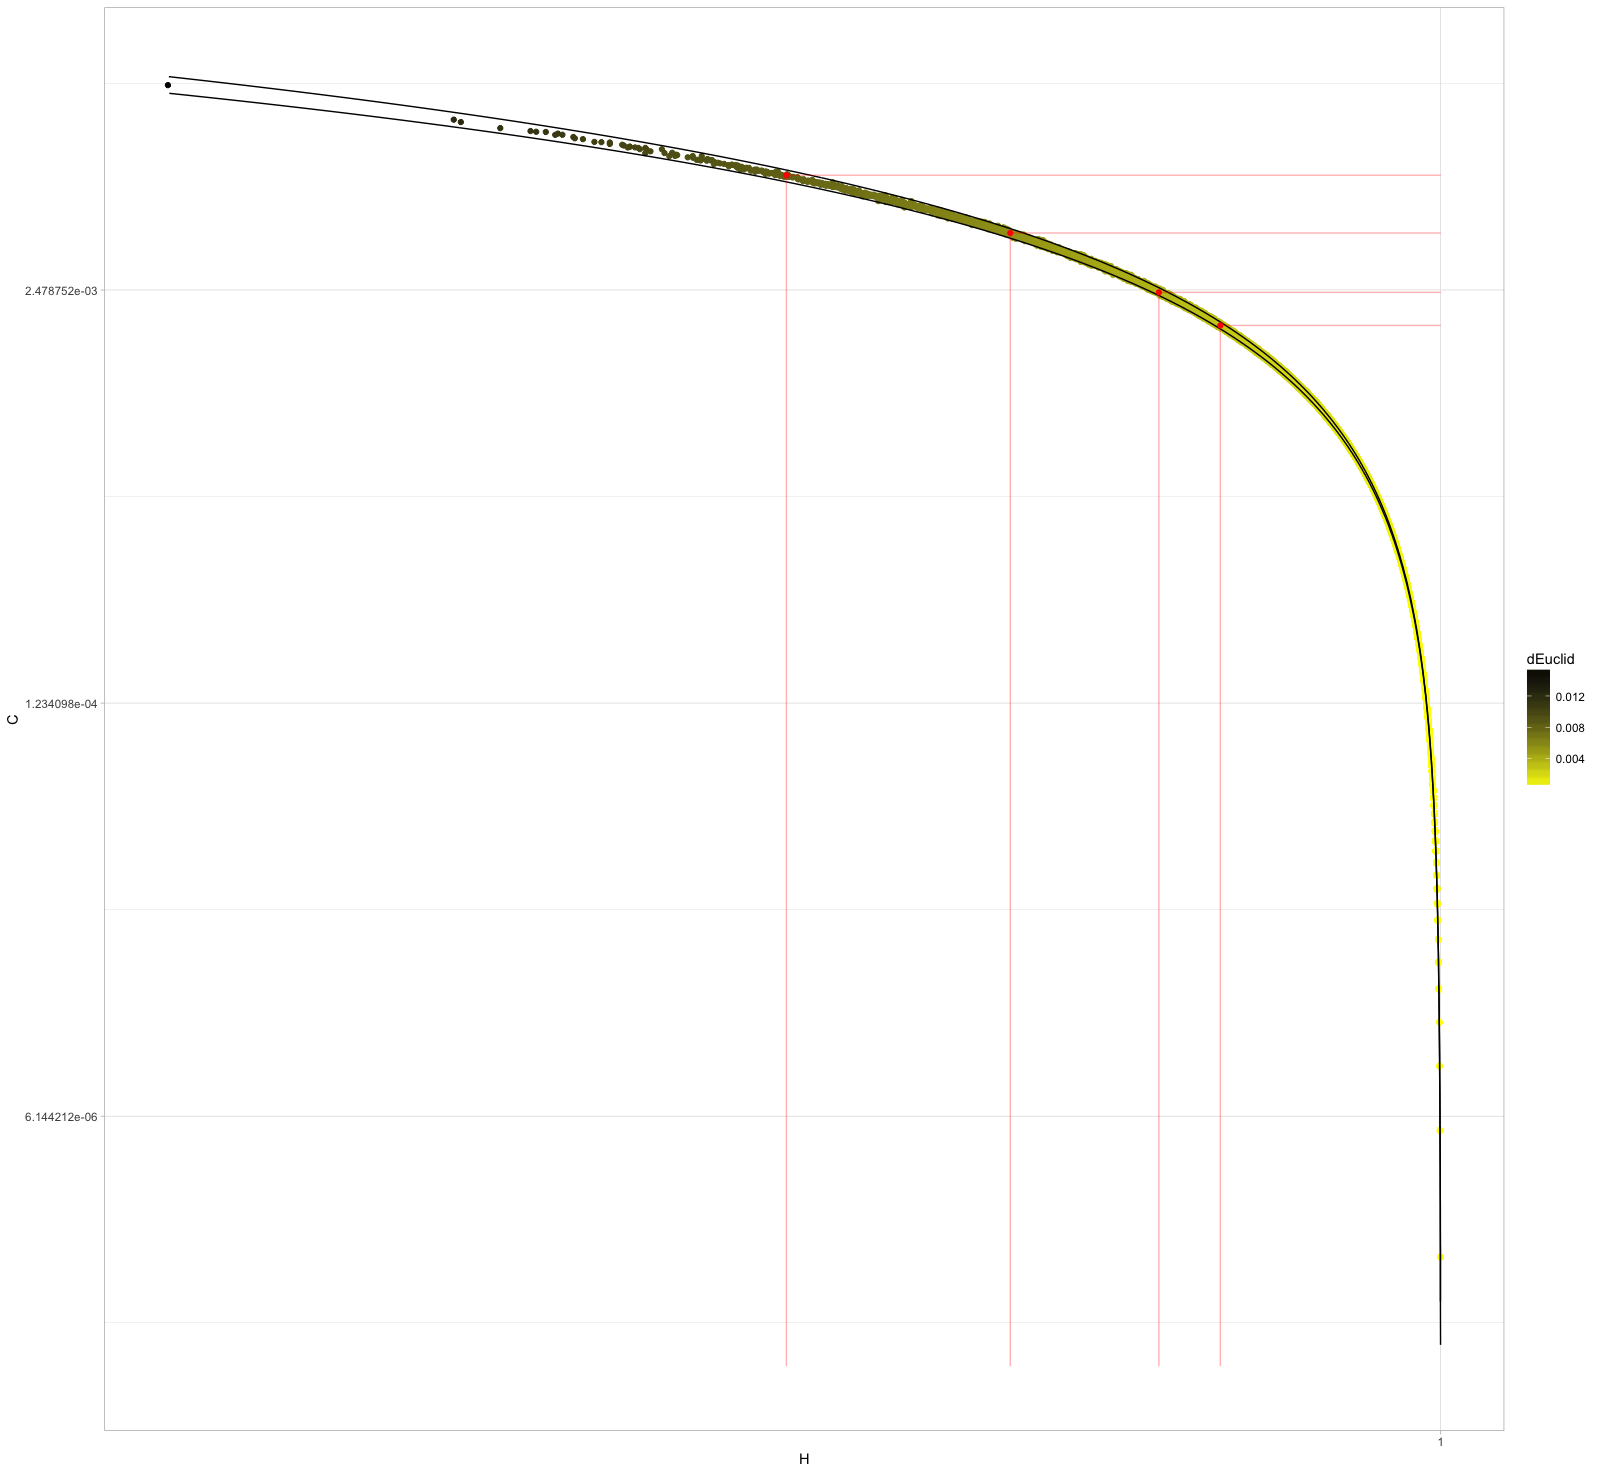
\includegraphics[width=.48\linewidth]{scatter1000D3t1_log}}
\caption{Diagramas de dispersão das sequências aleatórias para o caso $N=1.000$, $D=3$ e $\tau=1$.}\label{Fig:AleattD3tau1}
\end{figure}

A figura~\ref{Fig:QuantD3tau10log} mostra os padrões das sequências aleatórias para o caso $N=50.000$, $D=6$ e $\tau=50$ no plano Entropia-Complexidade, junto com os quantis de \SI{90}{\percent}, \SI{95}{\percent}, \SI{99}{\percent} e \SI{99,9}{\percent} em escala linear (figura~\ref{Fig:scatter50kD6t50}) e em escala logarítmica (figura~\ref{Fig:scatter50kD6t50_log}).

\begin{figure}
\centering
\subfigure[Escala linear\label{Fig:scatter50kD6t50}]{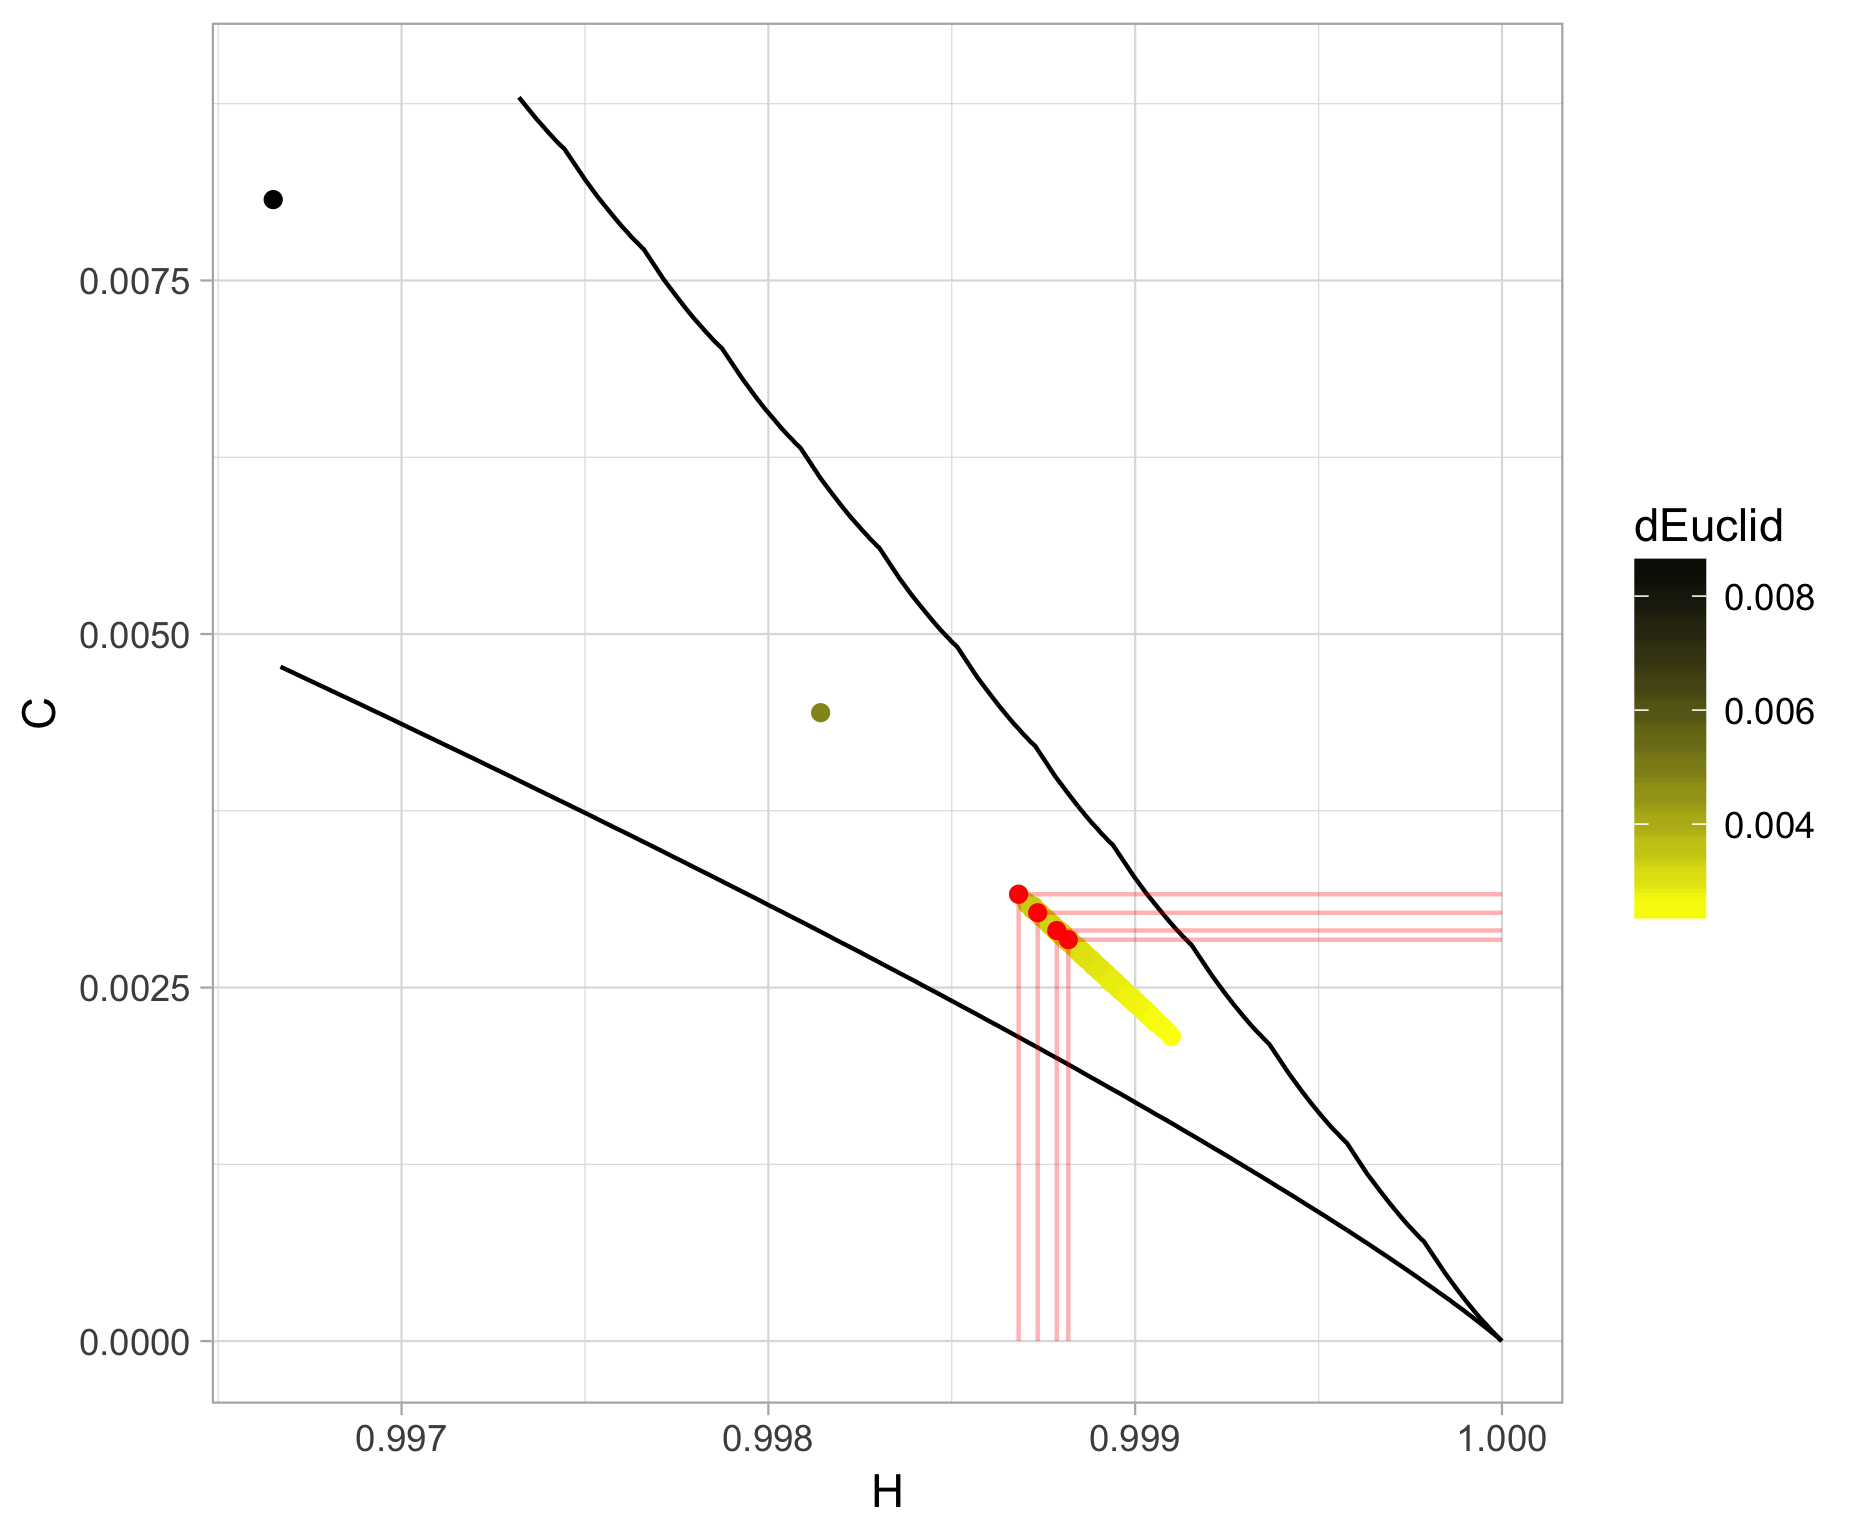
\includegraphics[width=.48\linewidth]{scatter50kD6t50}}
\subfigure[Escala logarítmica\label{Fig:scatter50kD6t50_log}]{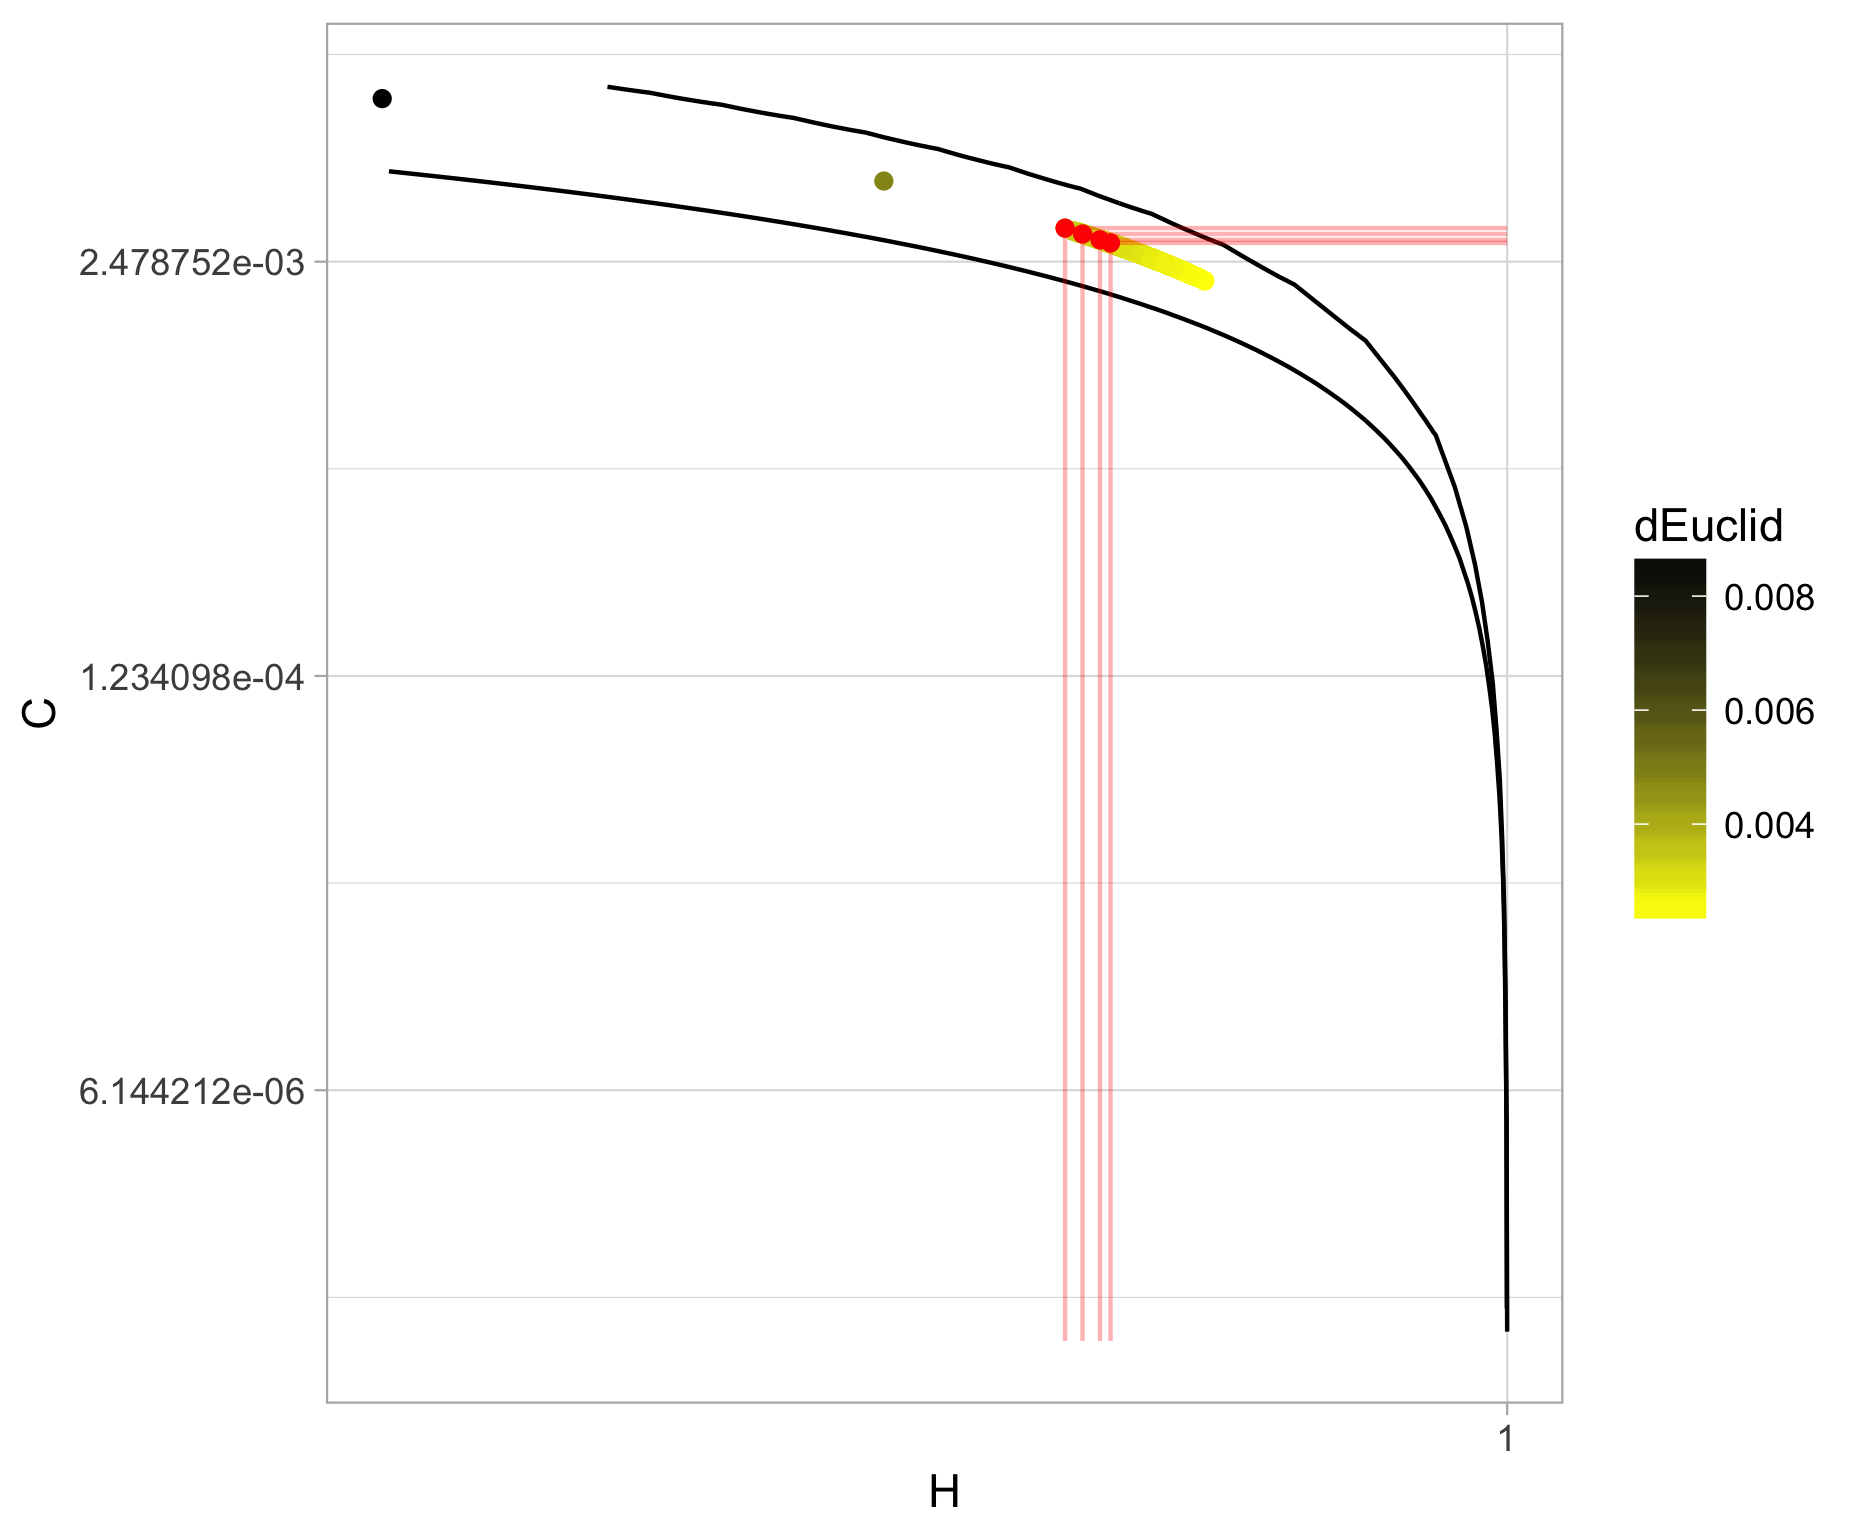
\includegraphics[width=.48\linewidth]{scatter50kD6t50_log}}
\caption{Diagramas de dispersão das sequências aleatórias para o caso $N=50.000$, $D=6$ e $\tau=50$.}\label{Fig:QuantD3tau10log}
\end{figure}

Nestas duas figuras, os pontos característicos foram desenhados com um gradiente de cores que vai do amarelo ao preto em função da distância ao ponto de referência.
Identificamos também os valores de Entropia e de Complexidade Estatística correspondentes a cada quantil de interesse.

Os resultados centrais dessa dissertação são exibidos nas figuras~\ref{Fig:Conf_Int_1k_T1}, \ref{Fig:Conf_Int_1k_T10}, 
\ref{Fig:Conf_Int_1k_30} e~\ref{Fig:Conf_Int_1k_T50} (os quantis de interesse para amostras de tamanho $1.000$ e $\tau=1, 10, 30, 50$), e nas figuras~\ref{Fig:Conf_Int_50k_T1}, \ref{Fig:Conf_Int_50k_T10},
\ref{Fig:Conf_Int_50k_30} e~\ref{Fig:Conf_Int_50k_T50} (os quantis de interesse para amostras de tamanho $50.000$ e $\tau=1, 10, 30, 50$).
Cada uma destas figuras inclui as quatro situações de $D=3, 4, 5, 6$.

Adicionalmente, aos gráficos são apresentadas tabelas \ref{tab:dEuclid_1000} e \ref{tab:dEuclid_50k} mostrando os valores da distância euclidiana dos pontos de interesse dos quantis ao ponto de referência.

%% N=1.000

\begin{table}[hbt]
	\centering
	\caption{Quantis das distâncias euclidianas para os valores de $D= 3, 4, 5, 6$ e $\tau=1, 10, 30, 50$ para sequências de $1.000$ observações.}\label{tab:dEuclid_1000}
	\begin{tabular}{ccccccc}
		\toprule
		$N=1.000$	&  $D$  &$\tau$  &\SI{90}{\percent}&\SI{95}{\percent}&\SI{99}{\percent}&\SI{99.9}{\percent}\\
		\midrule
		&  $3$ &  $ 1$ & 2.728065e-03  &  3.478919e-03  &  0.0053313857  &  0.0081048900 \\ 
		&  $3$ &  $10$ & 2.802528e-03  &  3.577539e-03  &  0.0054960059  &  0.0083091257 \\
		&  $3$ &  $30$ & 2.961344e-03  &  3.749702e-03  &  0.0056871429  &  0.0087472165 \\
		&  $3$ &  $50$ & 3.120298e-03  &  3.950138e-03  &  0.0059008109  &  0.0090272065 \\
		\midrule
		&  $4$ &  $ 1$ & 7.964076e-03  &  9.015899e-03  &  0.0112777244  &  0.0143372255 \\ 
		&  $4$ &  $10$ & 8.199472e-03  &  9.295153e-03  &  0.0116255590  &  0.0147762539 \\
		&  $4$ &  $30$ & 8.738506e-03  &  9.883617e-03  &  0.0123589751  &  0.0156235388 \\
		&  $4$ &  $50$ & 9.368242e-03  &  1.054840e-02  &  0.0131188349  &  0.0166817556 \\
		\midrule
		&  $5$ &  $ 1$ & 3.117067e-02  &  3.304803e-02  &  0.0366895915  &  0.0413215927 \\ 
		&  $5$ &  $10$ & 3.235895e-02  &  3.425898e-02  &  0.0380480169  &  0.0427998033 \\
		&  $5$ &  $30$ & 3.545788e-02  &  3.752600e-02  &  0.0417425086  &  0.0467667352 \\
		&  $5$ &  $50$ & 3.914194e-02  &  4.142425e-02  &  0.0459567507  &  0.0514563584 \\
		\midrule
		&  $6$ &  $ 1$ & 1.891794e-01  &  1.923893e-01  &  0.1984529319  &  0.2050583463 \\
		&  $6$ &  $10$ & 1.975446e-01  &  2.007669e-01  &  0.2069269144  &  0.2139321164 \\
		&  $6$ &  $30$ & 2.185870e-01  &  2.218804e-01  &  0.2280312709  &  0.2345272440 \\
		&  $6$ &  $50$ & 2.431686e-01  &  2.464034e-01  &  0.2526103765  &  0.2596196960 \\
		\bottomrule
	\end{tabular}
\end{table}

\begin{figure}
	\centering
	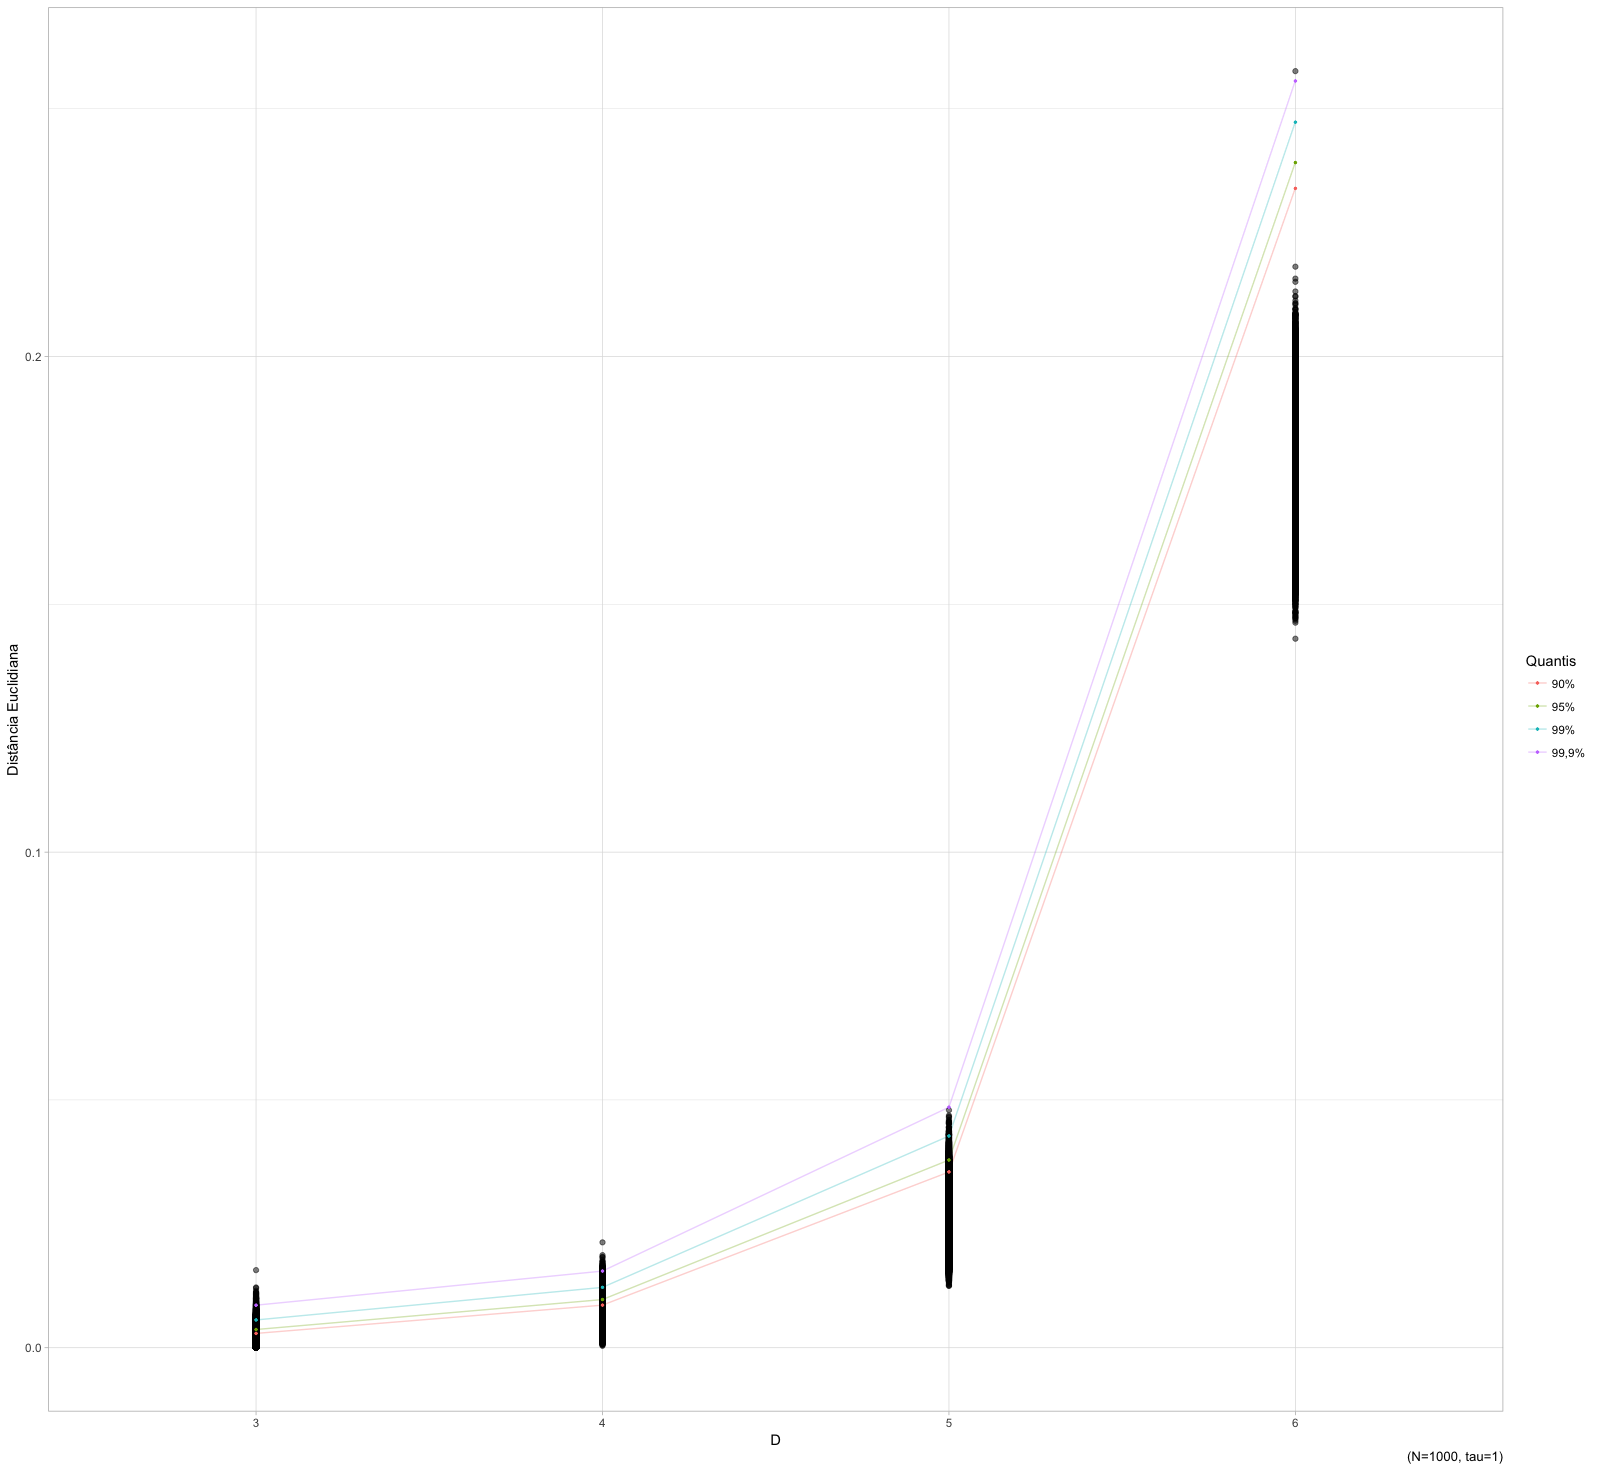
\includegraphics[width=1\linewidth]{Conf_Int_1k_T1_noMT}
	\caption{Intervalos de confiança para o caso $N=1.000$ e $\tau=1$.}\label{Fig:Conf_Int_1k_T1}
\end{figure}

\begin{figure}
	\centering
	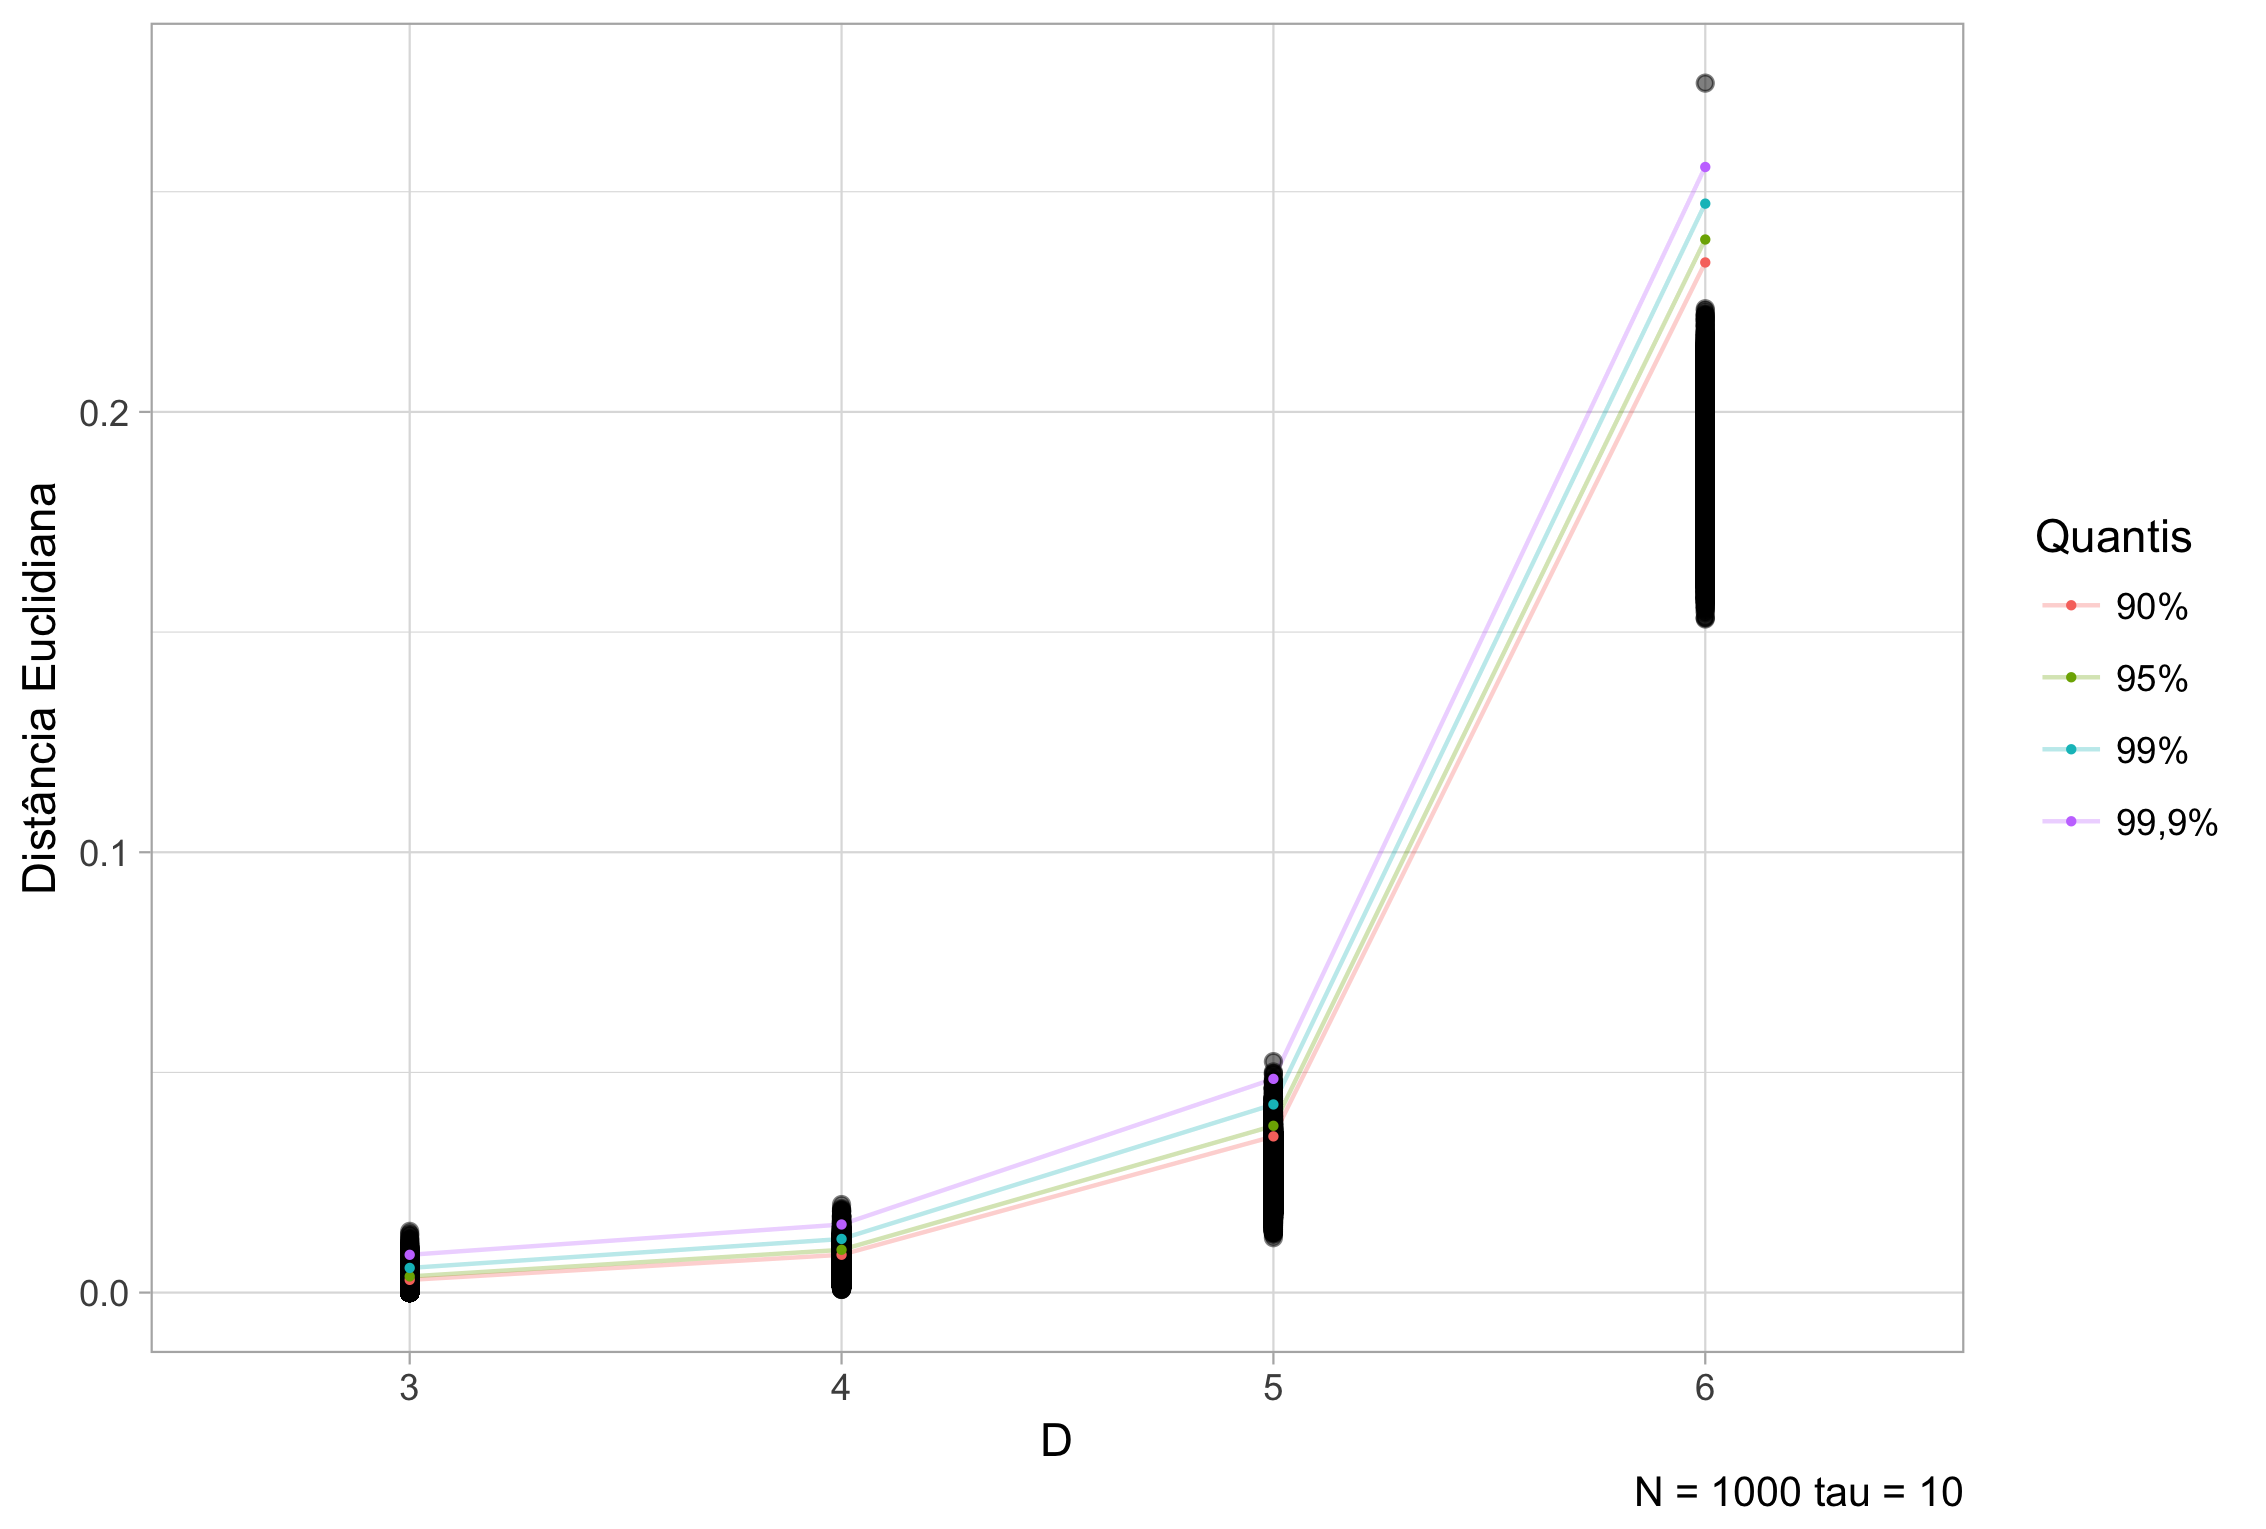
\includegraphics[width=1\linewidth]{Conf_Int_1k_T10_noMT}
	\caption{Intervalos de confiança para o caso $N=1.000$ e $\tau=10$.}\label{Fig:Conf_Int_1k_T10}
\end{figure}

\begin{figure}
	\centering
	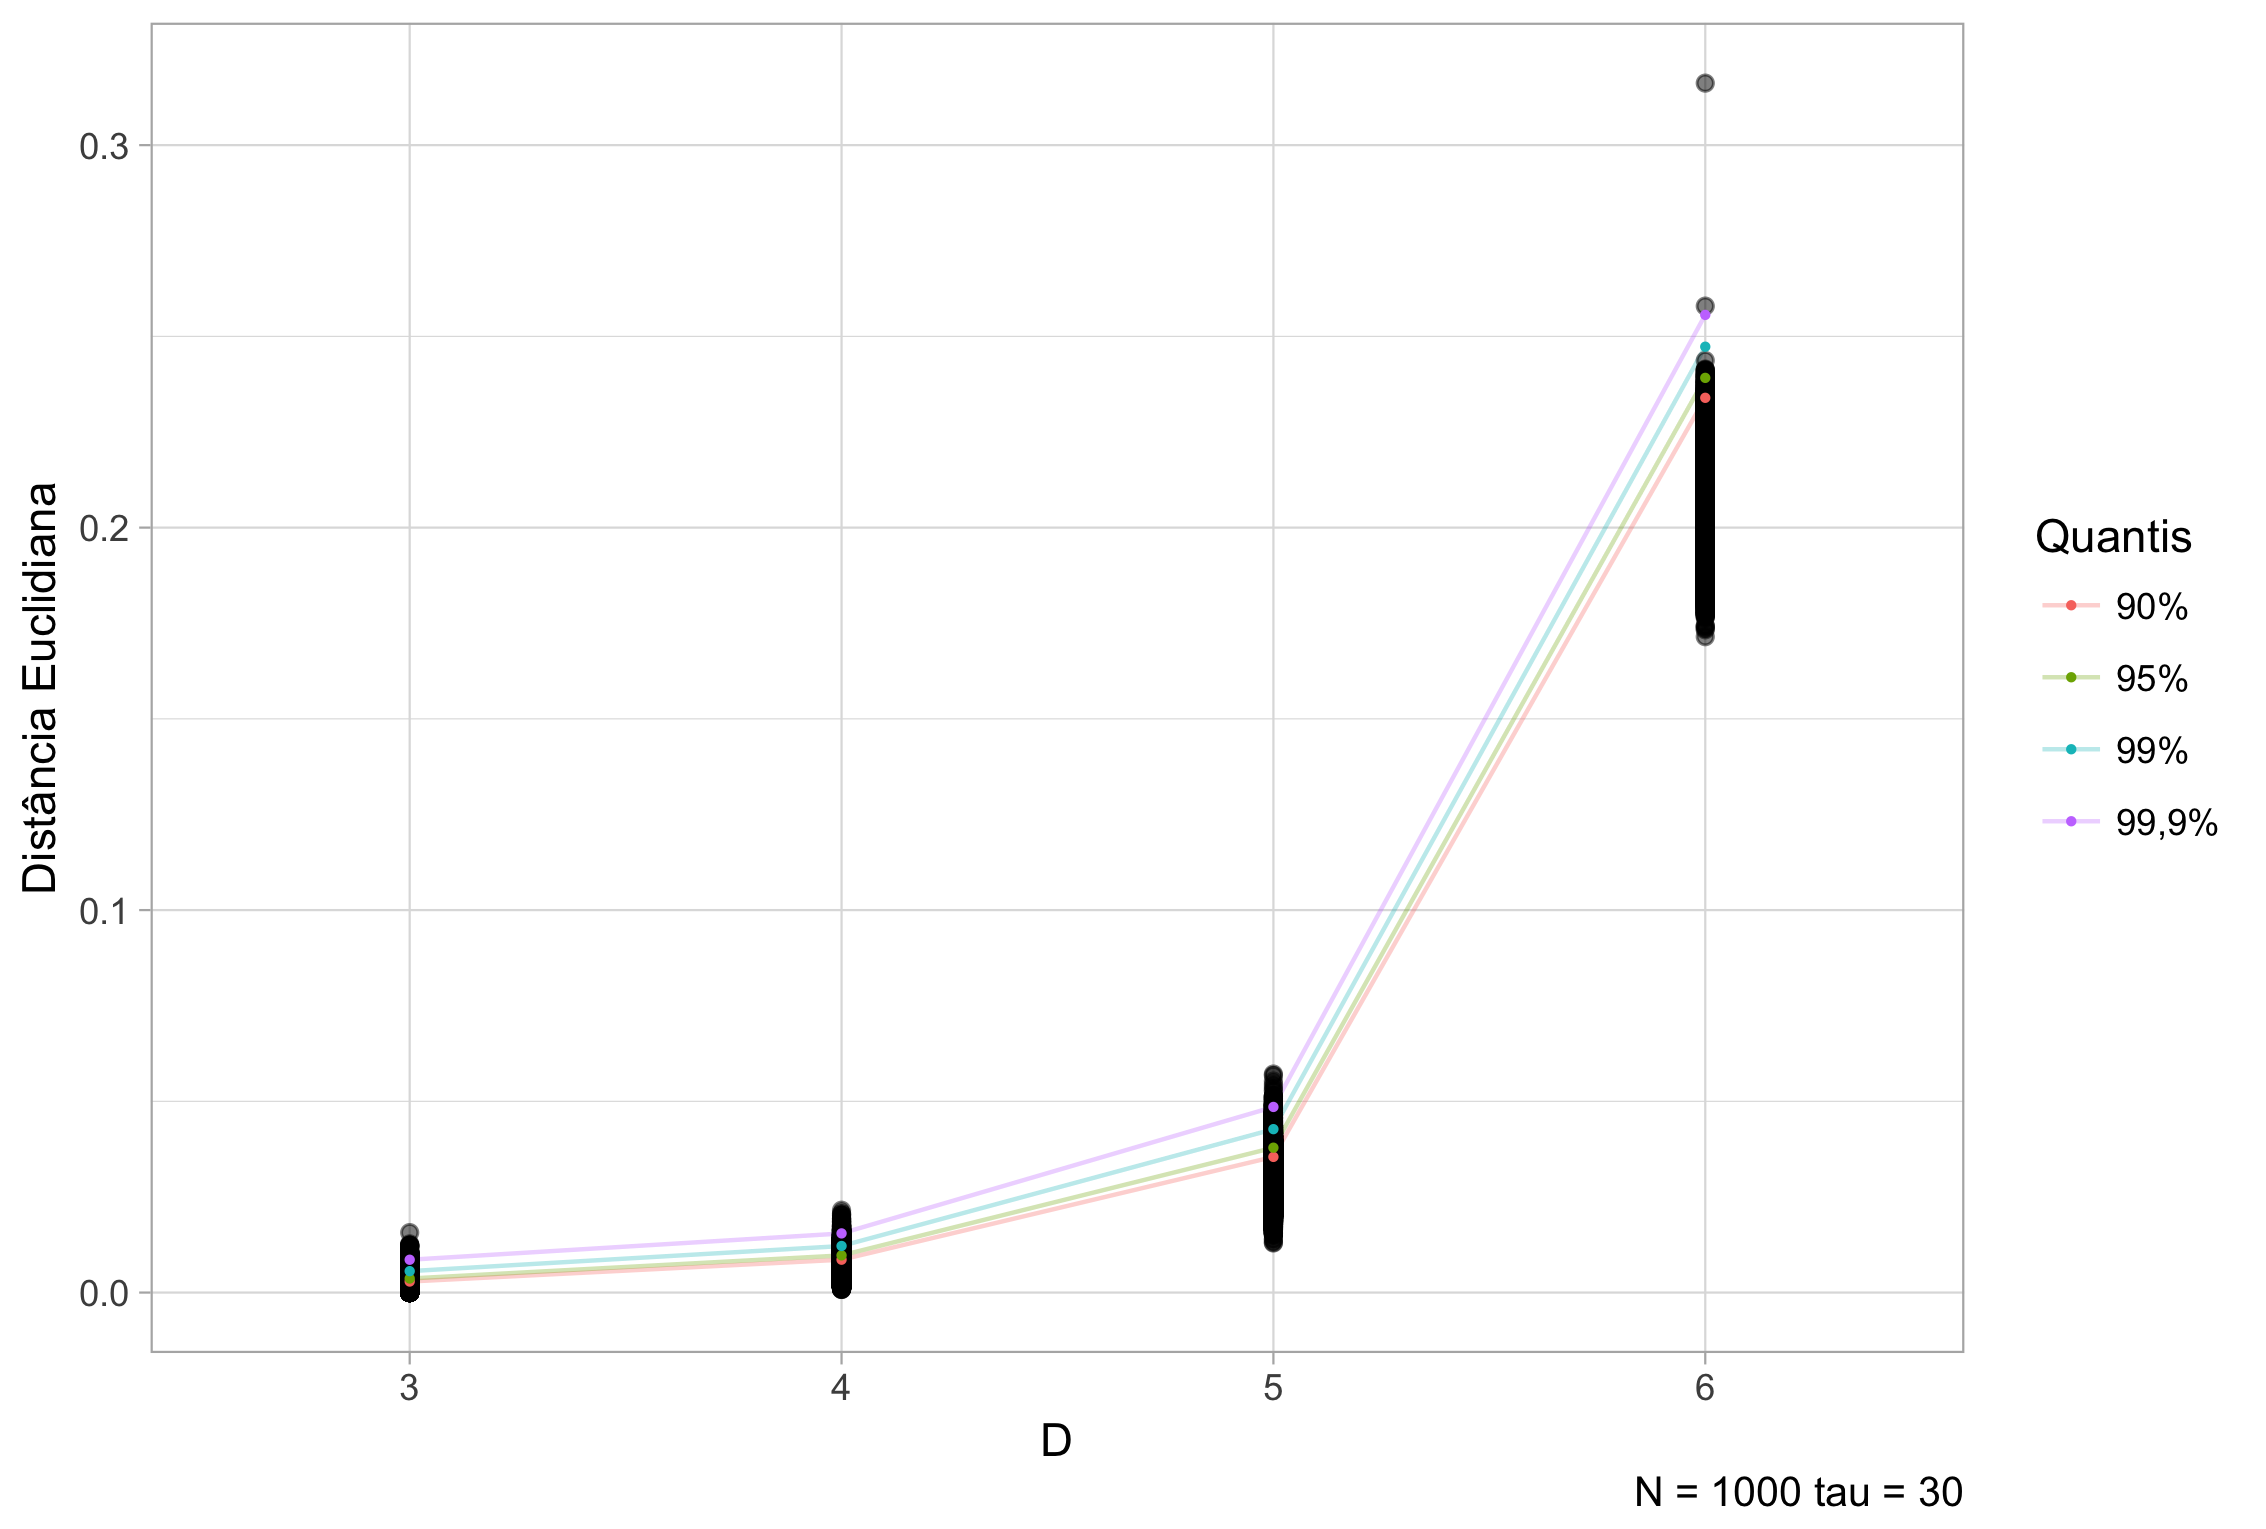
\includegraphics[width=1\linewidth]{Conf_Int_1k_T30_noMT}
	\caption{Intervalos de confiança para o caso $N=1.000$ e $\tau=30$.}\label{Fig:Conf_Int_1k_30}
\end{figure}

\begin{figure}
	\centering
	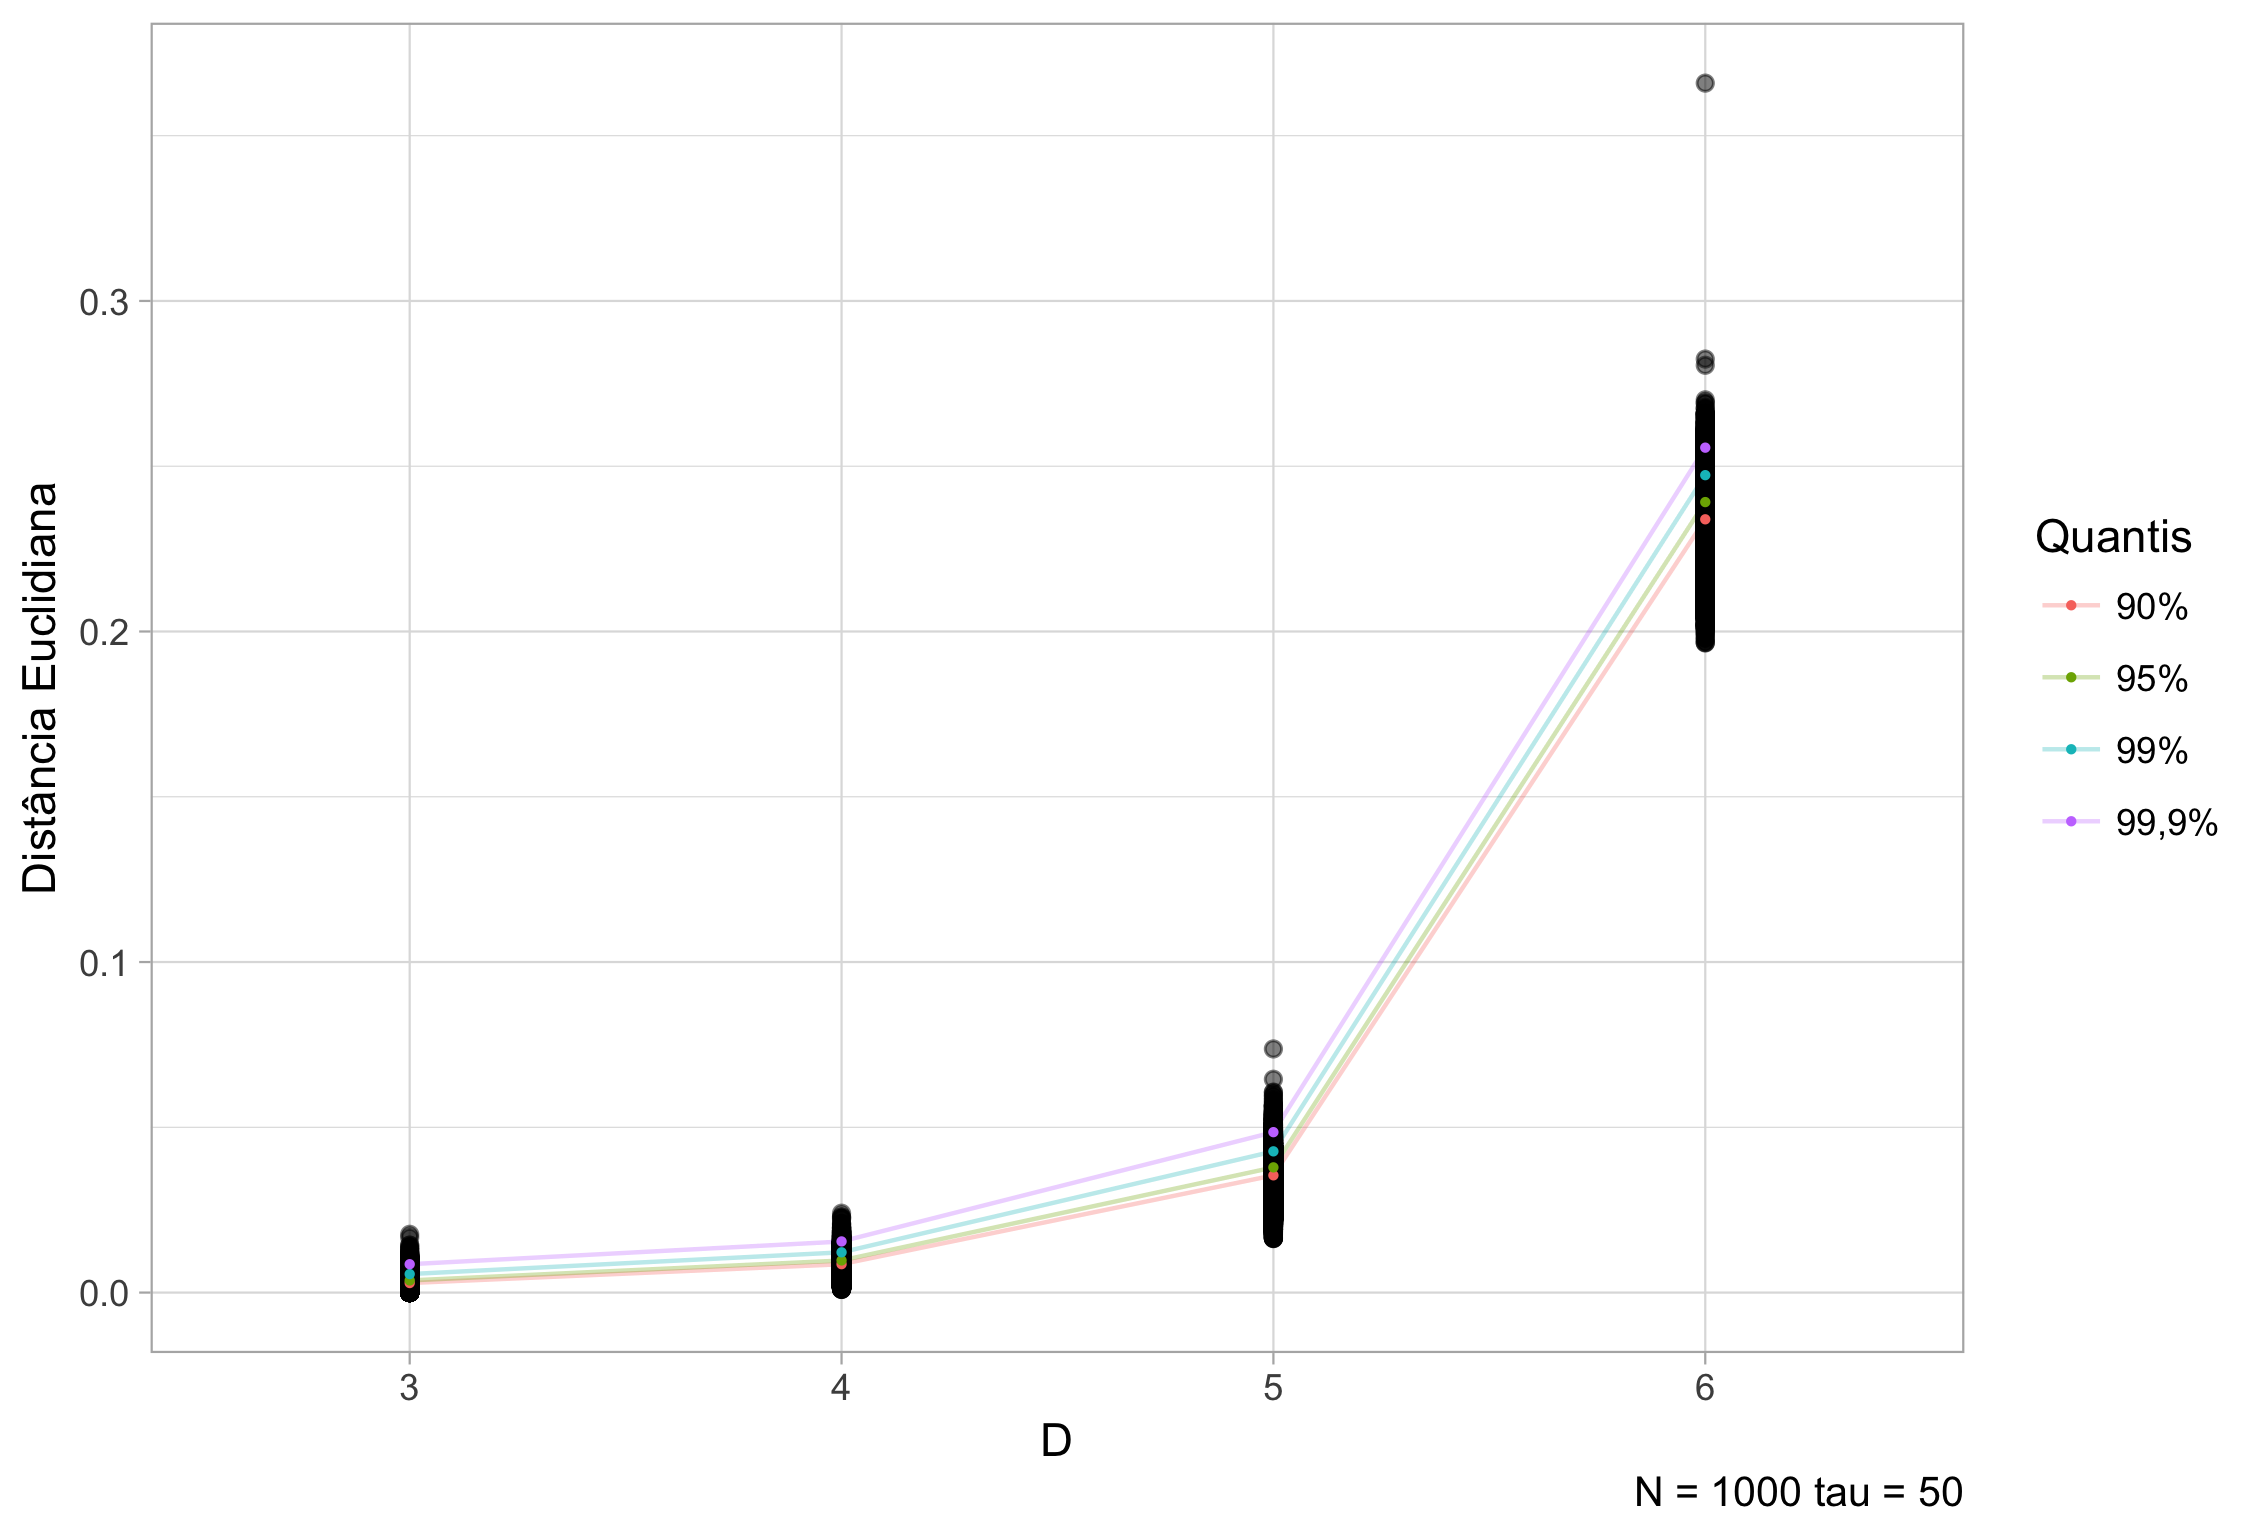
\includegraphics[width=1\linewidth]{Conf_Int_1k_T50_noMT}
	\caption{Intervalos de confiança para o caso $N=1.000$ e $\tau=50$.}\label{Fig:Conf_Int_1k_T50}
\end{figure}
%%

%% N=50.000

\begin{table}[hbt]
	\centering
	\caption{Quantis das distâncias euclidianas para os valores de $D= 3, 4, 5, 6$ e $\tau=1, 10, 30, 50$ para sequências de $50.000$ observações.}\label{tab:dEuclid_50k}
	\begin{tabular}{ccccccc}
		\toprule
		$N = 50.000$	&  $D$  &$\tau$  &\SI{90}{\percent}&\SI{95}{\percent}&\SI{99}{\percent}&\SI{99.9}{\percent}\\ 
		\midrule
		&  $3$  &  $ 1$  &  5.407679e-05  &  7.015910e-05  &  0.0001178519  &  0.0001917689 \\ 
		&  $3$  &  $10$  &  5.636160e-05  &  7.130762e-05  &  0.0001000853  &  0.0001585019 \\
		&  $3$  &  $30$  &  5.731458e-05  &  7.245769e-05  &  0.0001101931  &  0.0001580179 \\
		&  $3$  &  $50$  &  5.951595e-05  &  7.541980e-05  &  0.0001093136  &  0.0001983728 \\ 
		\midrule
		&  $4$  &  $ 1$  &  1.589081e-04  &  1.818144e-04  &  0.0002250318  &  0.0003038889 \\ 
		&  $4$  &  $10$  &  1.588585e-04  &  1.790301e-04  &  0.0002264259  &  0.0002903681 \\
		&  $4$  &  $30$  &  1.631504e-04  &  1.863802e-04  &  0.0002330694  &  0.0002893557 \\
		&  $4$  &  $50$  &  1.619028e-04  &  1.809200e-04  &  0.0002311957  &  0.0003017229 \\ 
		\midrule
		&  $5$  &  $ 1$  &  6.062508e-04  &  6.389830e-04  &  0.0007179730  &  0.0008832568 \\ 
		&  $5$  &  $10$  &  5.985032e-04  &  6.289105e-04  &  0.0007041024  &  0.0007855387 \\
		&  $5$  &  $30$  &  6.040569e-04  &  6.400727e-04  &  0.0007268196  &  0.0008213228 \\
		&  $5$  &  $50$  &  6.055769e-04  &  6.381391e-04  &  0.0007134216  &  0.0008042788 \\ 
		\midrule
		&  $6$  &  $ 1$  &  3.071590e-03  &  3.150152e-03  &  0.0033104814  &  0.0035923810 \\ 
		&  $6$  &  $10$  &  3.050841e-03  &  3.117779e-03  &  0.0032553996  &  0.0033734229 \\
		&  $6$  &  $30$  &  3.066360e-03  &  3.129649e-03  &  0.0032669327  &  0.0034581195 \\
		&  $6$  &  $50$  &  3.074748e-03  &  3.147889e-03  &  0.0032828968  &  0.0034178859 \\
		\bottomrule
	\end{tabular}
\end{table}

\begin{figure}
	\centering
	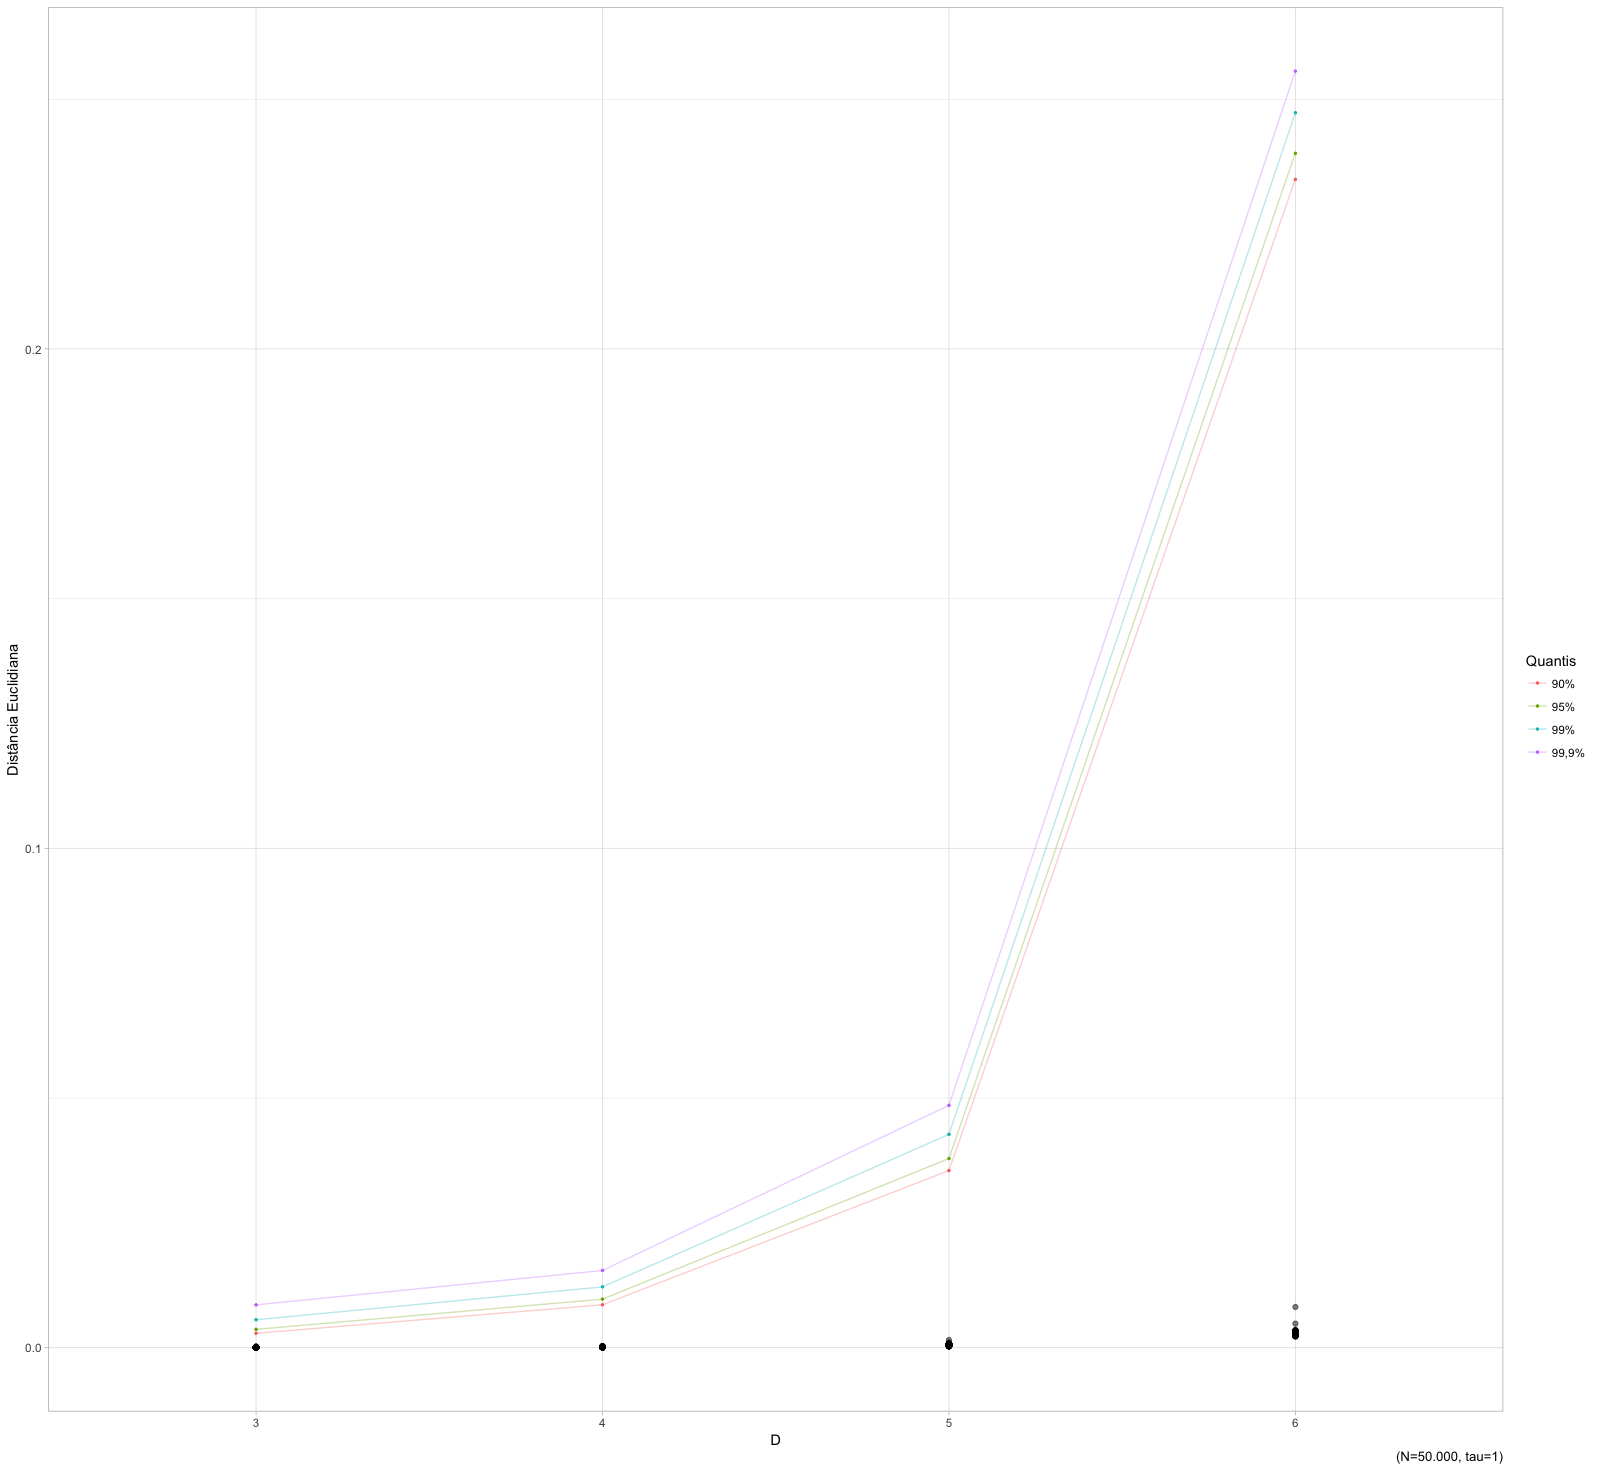
\includegraphics[width=1\linewidth]{Conf_Int_50k_T1_noMT}
	\caption{Intervalos de confiança para o caso $N=50.000$ e $\tau=1$.}\label{Fig:Conf_Int_50k_T1}
\end{figure}

\begin{figure}
	\centering
	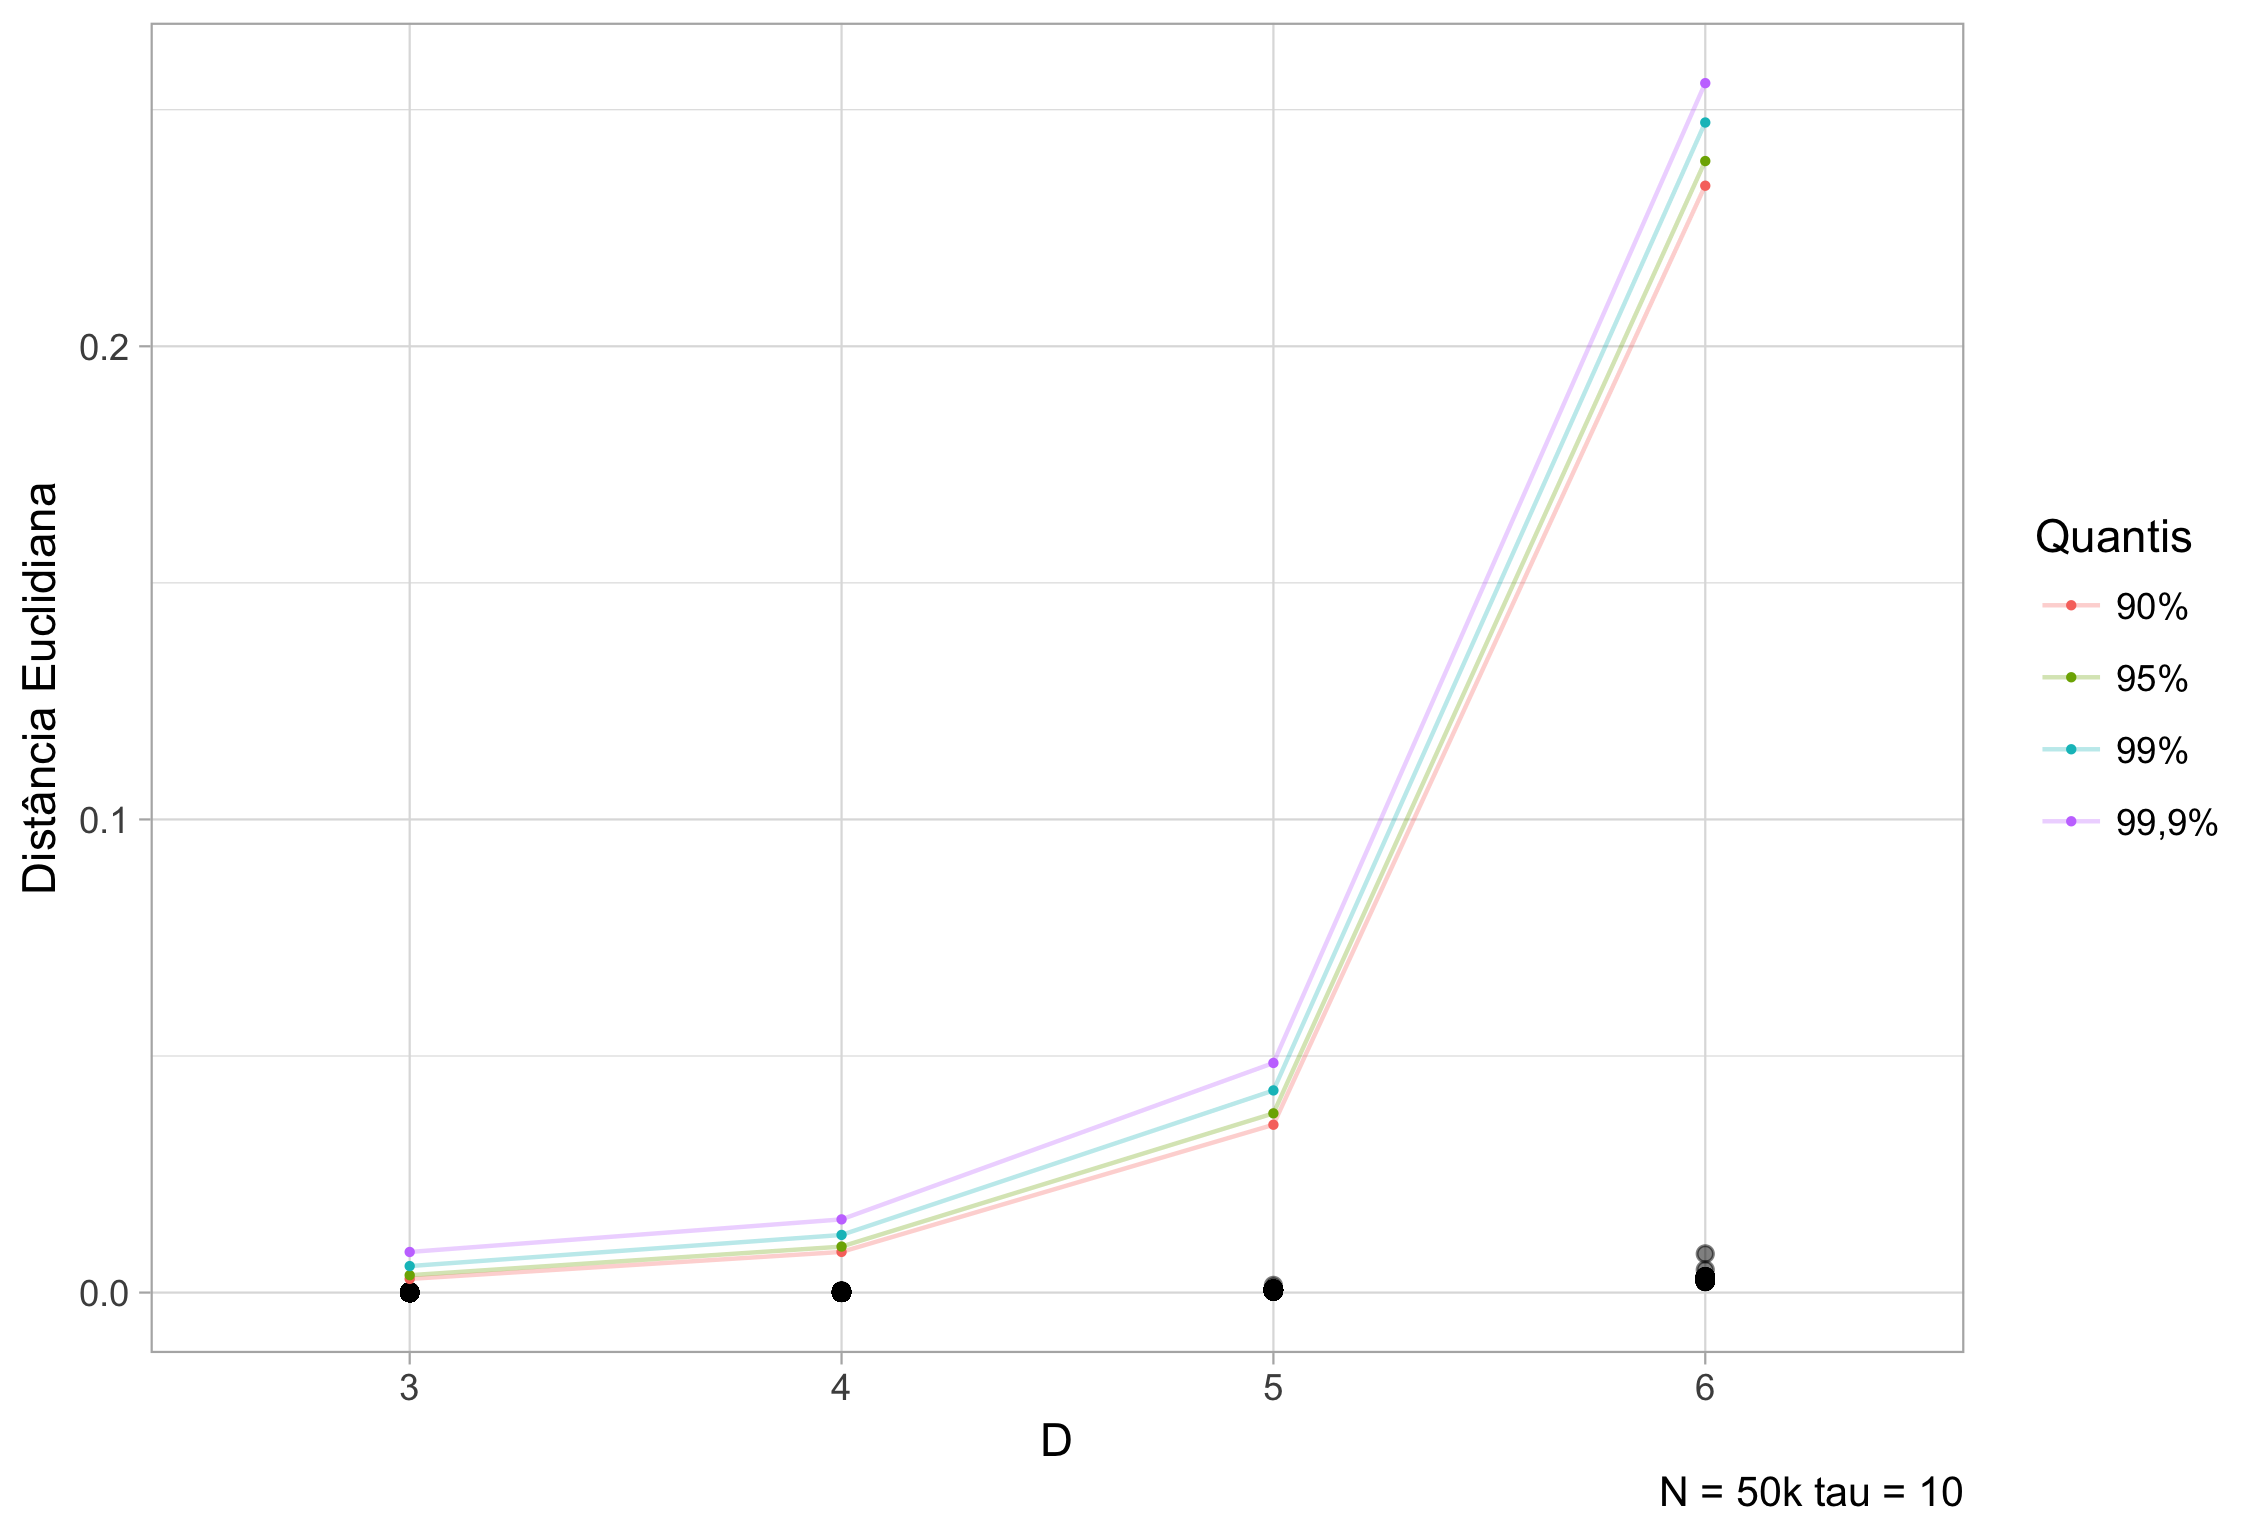
\includegraphics[width=1\linewidth]{Conf_Int_50k_T10_noMT}
	\caption{Intervalos de confiança para o caso $N=50.000$ e $\tau=10$.}\label{Fig:Conf_Int_50k_T10}
\end{figure}

\begin{figure}
	\centering
	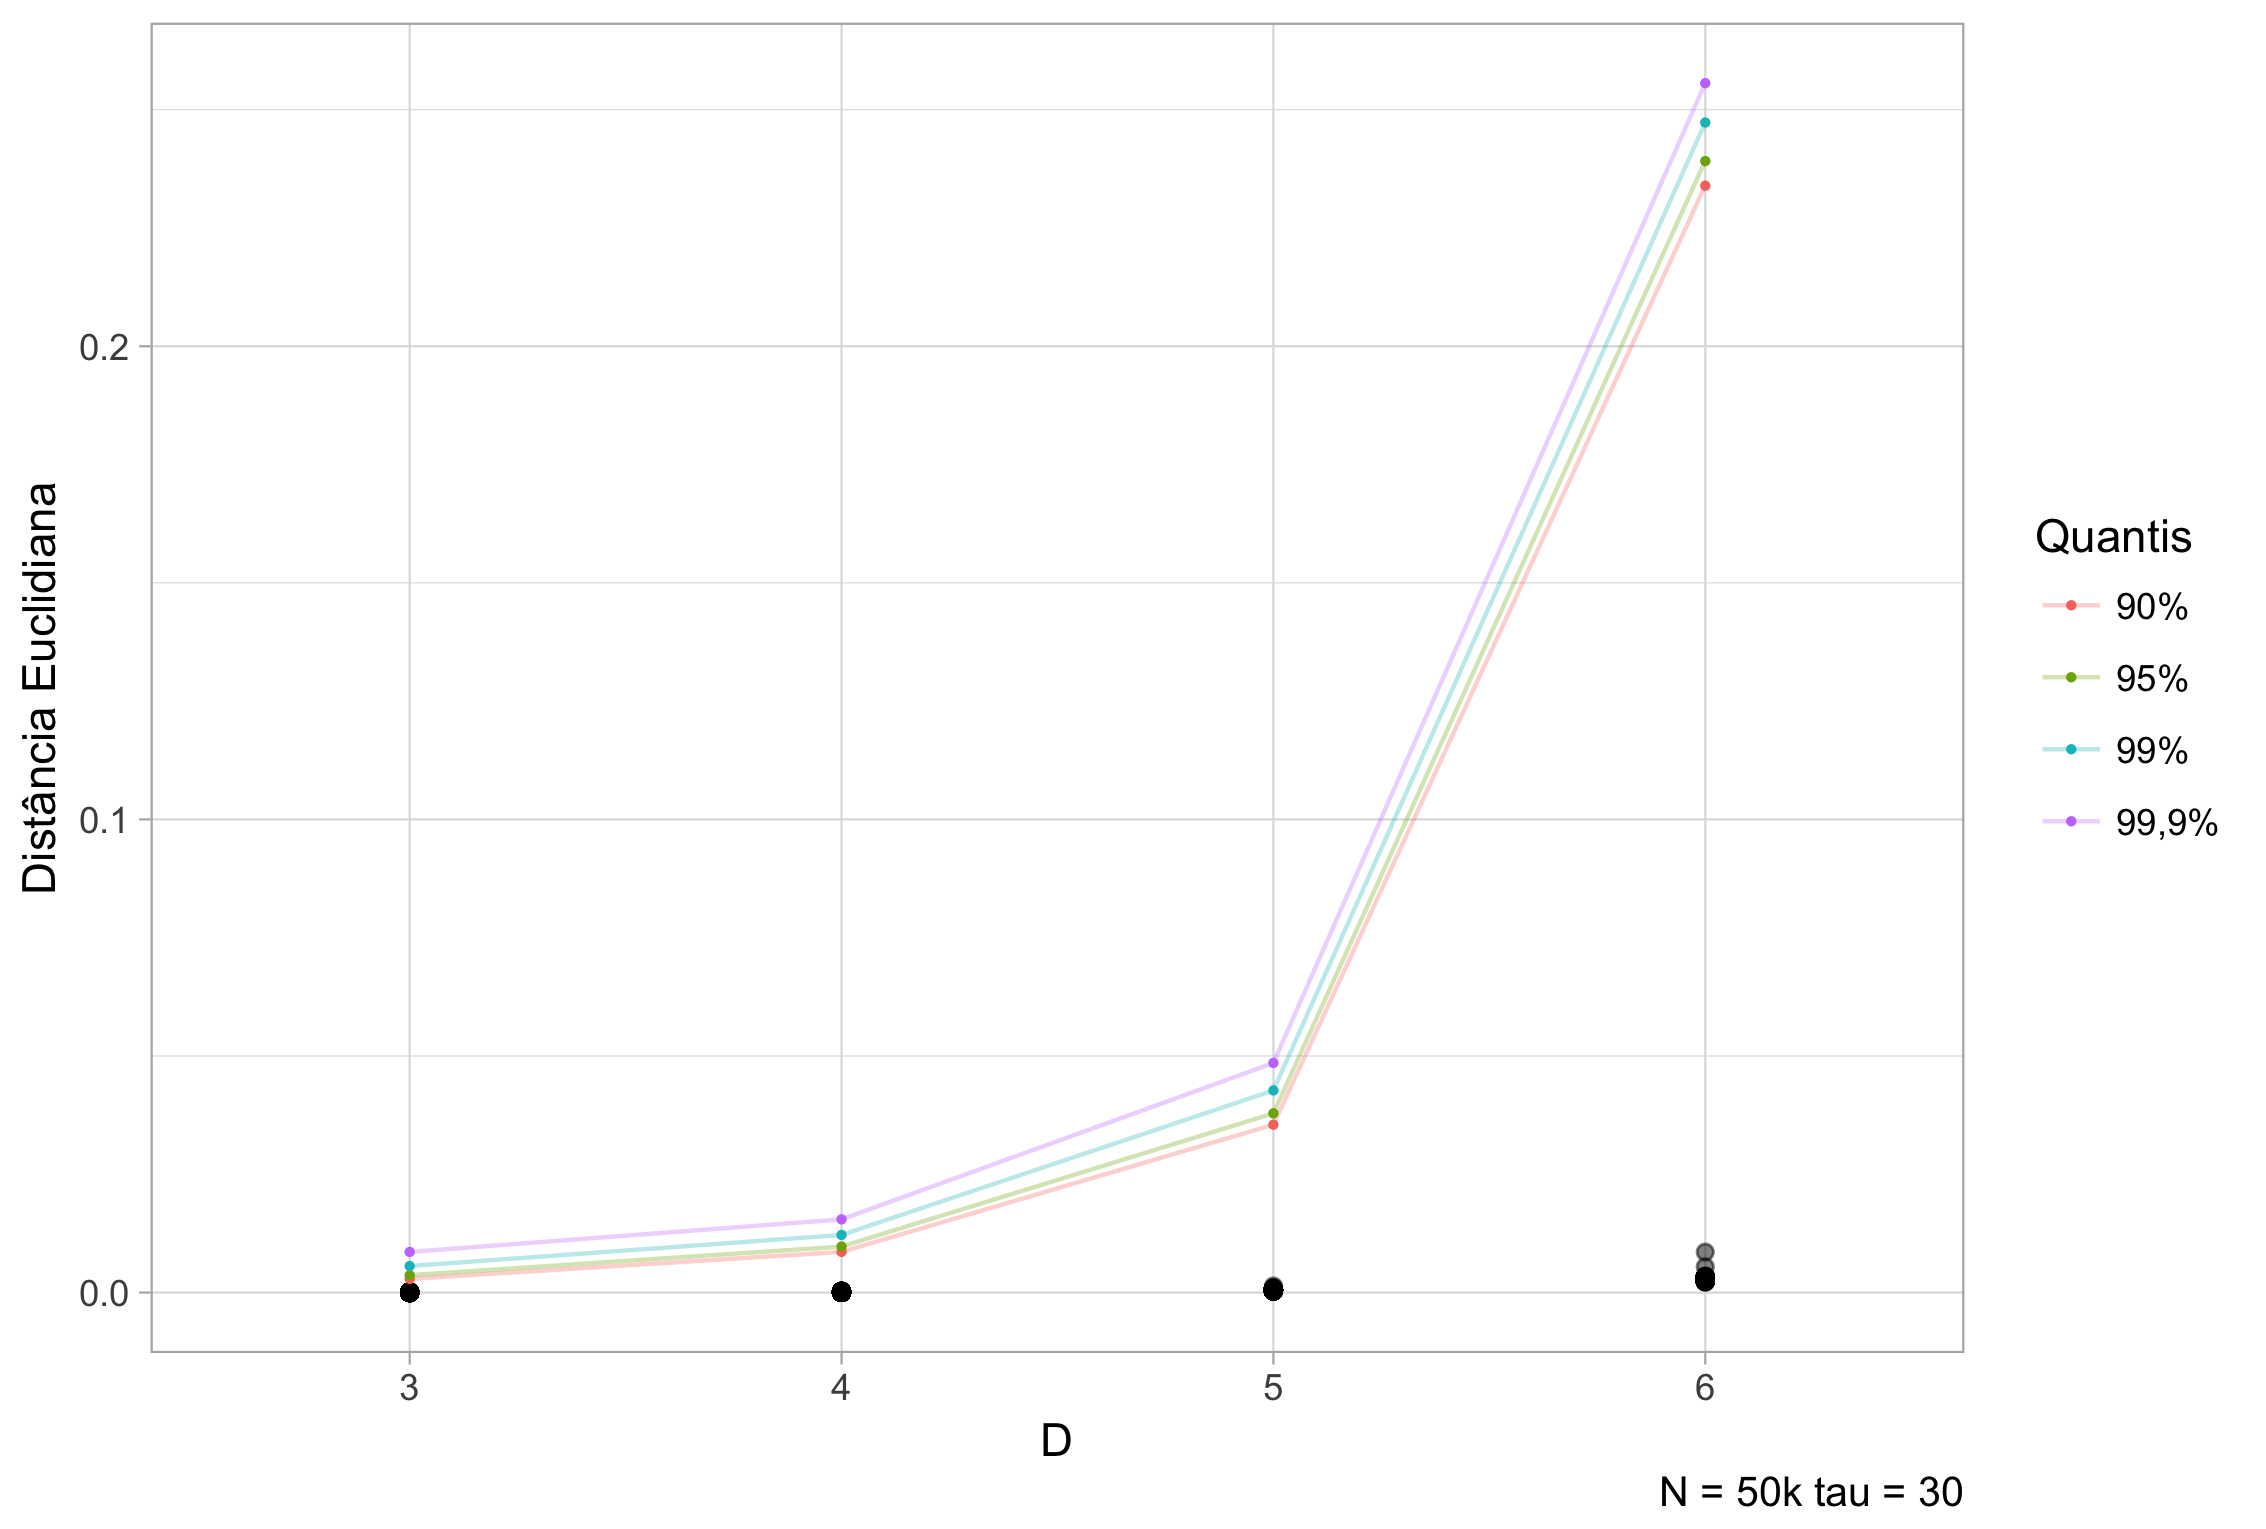
\includegraphics[width=1\linewidth]{Conf_Int_50k_T30_noMT}
	\caption{Intervalos de confiança para o caso $N=50.000$ e $\tau=30$.}\label{Fig:Conf_Int_50k_30}
\end{figure}

\begin{figure}
	\centering
	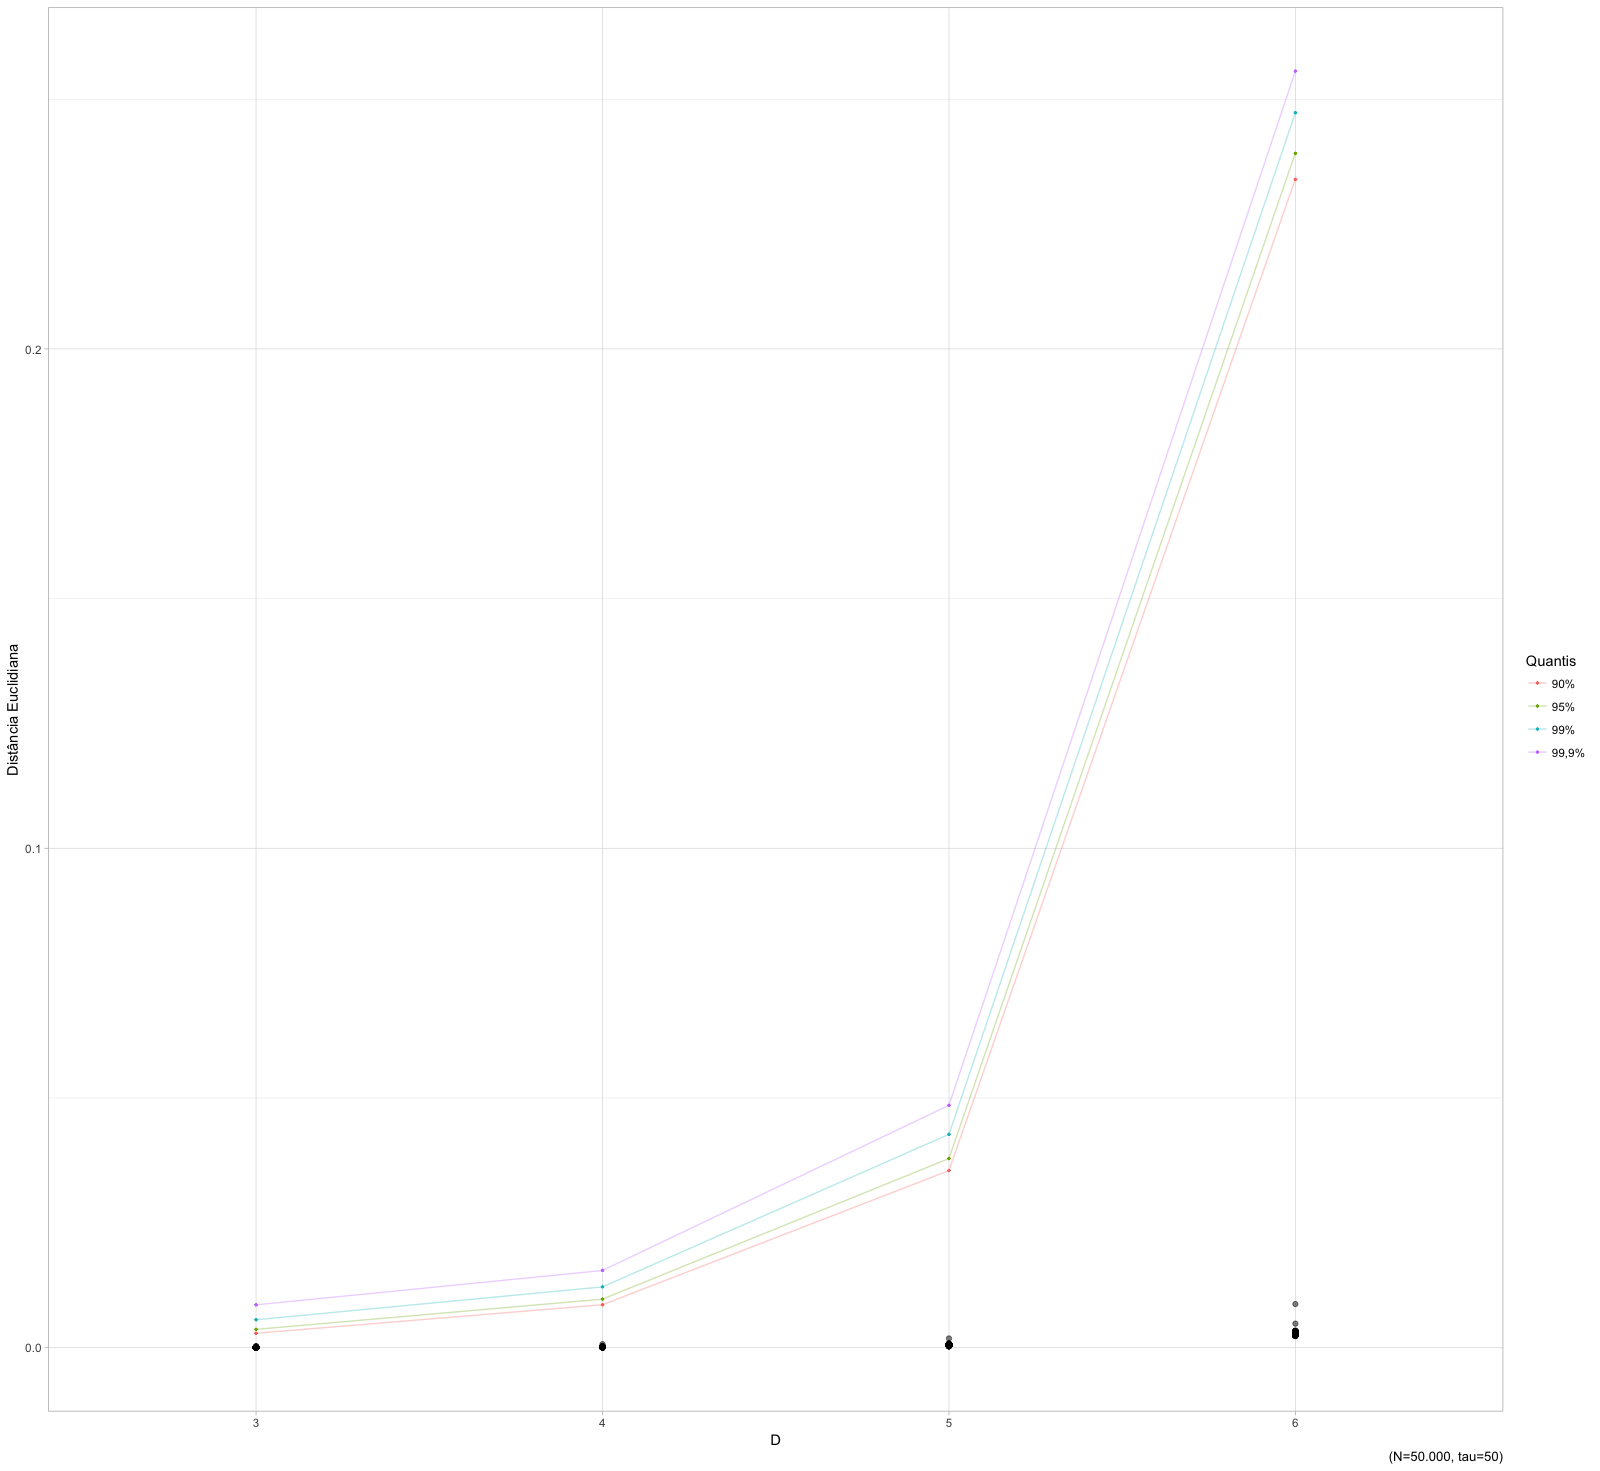
\includegraphics[width=1\linewidth]{Conf_Int_50k_T50_noMT}
	\caption{Intervalos de confiança para o caso $N=50.000$ e $\tau=50$.}\label{Fig:Conf_Int_50k_T50}
\end{figure}
%%

% % % ACF Coloque na seguinte sequência: tabela 1000, gráficos, tabela 50000, gráficos

\section{Aplicações}

Nesta seção mostramos a aplicação da nossa proposta a sequências de tamanho \num{50000}.

Utilizando a metodologia descrita, aplicamos o teste a uma seqência de \num{50000} observações produzidas pelos geradores Mersenne-Twister e Randu, além de séries não estacionárias, estacionárias e mapas logísticos, todos com a mesma dimensão.

Os resultados de aplicar a nossa abordagem às sequências oriundas dos geradores de números pseudoaleatórios podem ser observados na figura~\ref{fig:ConfInt_PRNGs}: Mersenne-Twister na figura~\ref{ConfidInt__MT_1k_t10} Randu na figura~\ref{ConfidInt__Randu_1k_t10}.
Para obter as sequências de Mersenne Twister utilizou-se a implementação interna do $R$~\ref{code:MersenneTwister},
já para as seqências de Randu foi implementada  função~\ref{code:Randu}.

\begin{figure}
	\centering
	\subfigure[Mersenne Twister. \label{ConfidInt__MT_1k_t10}]{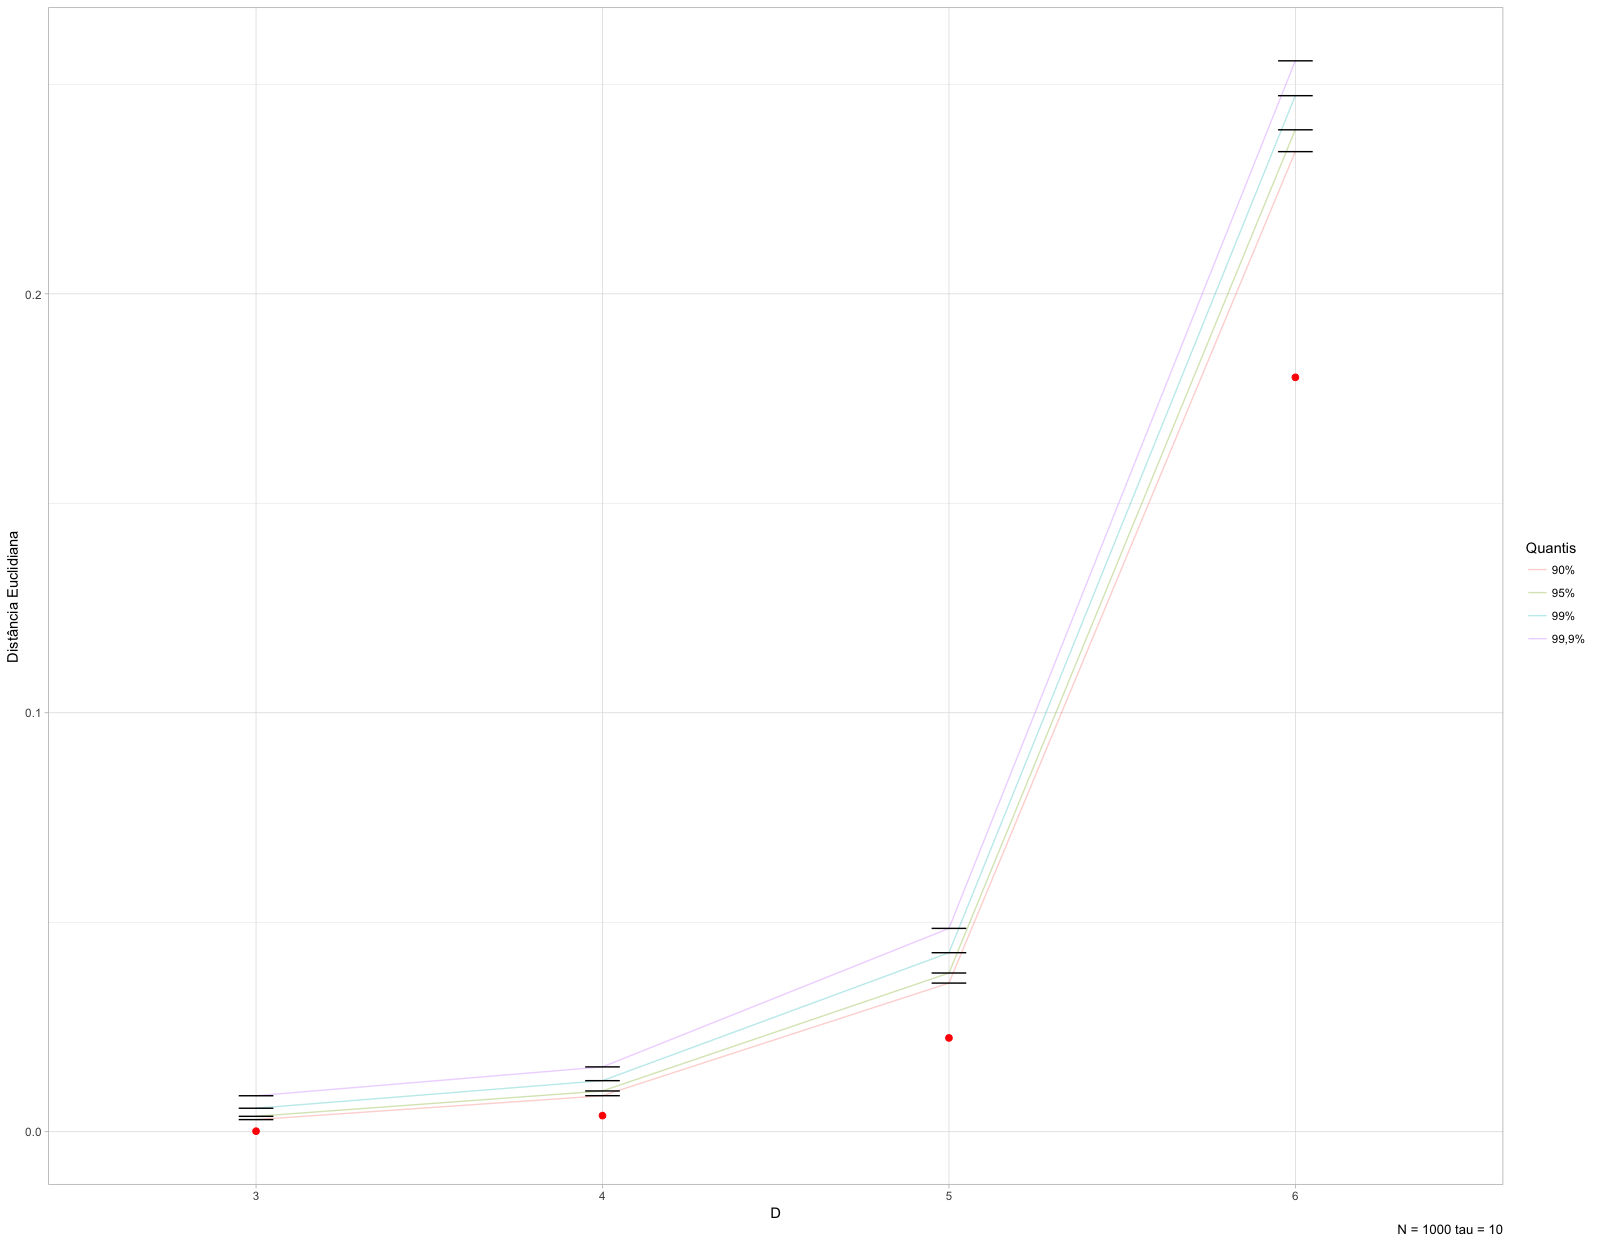
\includegraphics[width=.48\linewidth]{ConfidInt__MT_1k_t10}}
	\subfigure[Randu. \label{ConfidInt__Randu_1k_t10}]{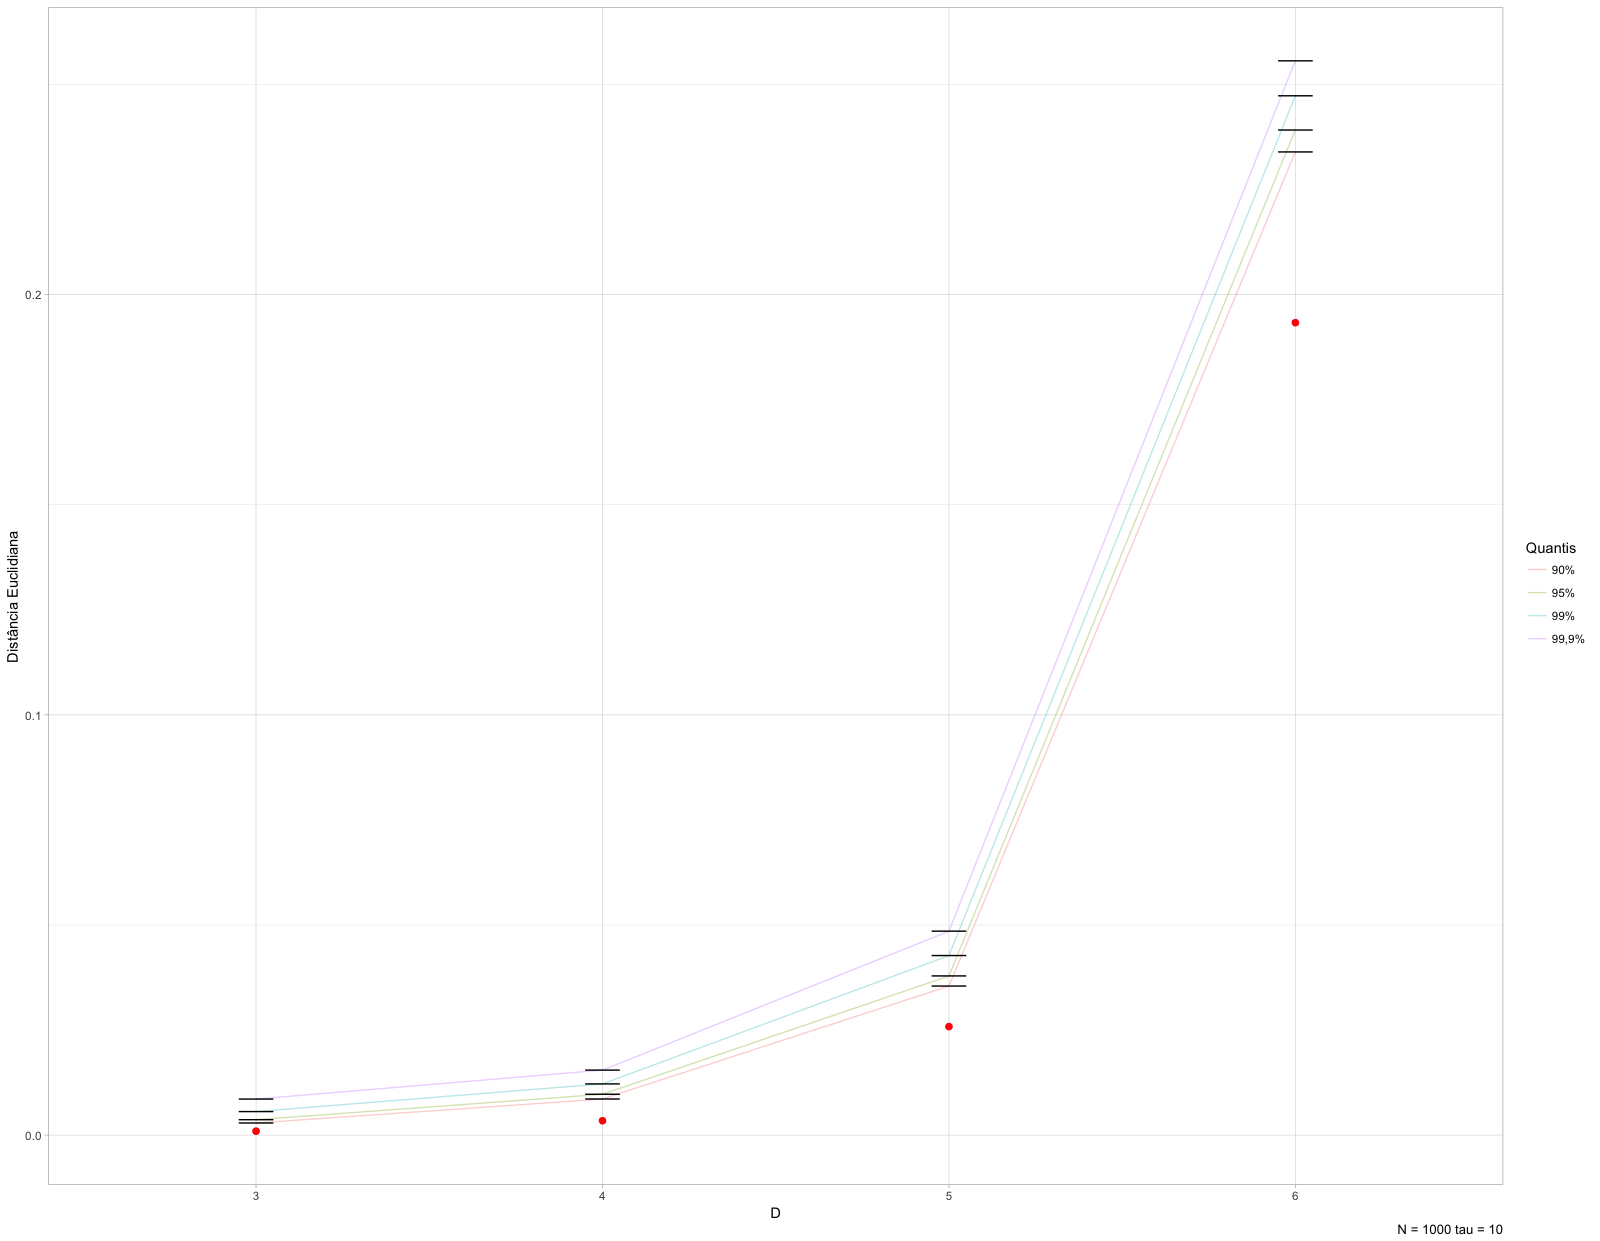
\includegraphics[width=.48\linewidth]{ConfidInt__Randu_1k_t10}}
	\caption{Aplicação do teste aos pontos de Mersenne-Twister e Randu}\label{fig:ConfInt_PRNGs}
\end{figure}

As figuras~\ref{ConfidInt__MT_1k_t10} e~\ref{ConfidInt__Randu_1k_t10} mostram que a nossa técnica não é capaz de identificar desvios significativos da hipótese dessas duas fontes de dados não produzirem ocorrências de variáveis independentes e identicamente distribuídas.
Embora já tenhamos mostrado evidências nesse sentido, através da figura~\ref{fig:3DRandu} para Randu e dos testes de Kolmogorov-Smirnov para o gerador Mersenne-Twister (tabelas~\ref{tab:KS_1000} e~\ref{tab:KS_50k}), as distâncias dos pontos característicos ao ponto de referência é inferior aos limites calculados para a rejeição da hipótese.
Isso se deve ao poder limitado do teste, característica que será investigada em futuros trabalhos.

A seguir, geramos sequências estocásticas com estrutura de autocorrelação: uma estacionária (ruído gaussiano filtrado) e uma não estacionária (uma trajetória de movimento browniano).

A aplicação do teste à sequência obtida pelo método de séries não estacionárias pode ser observada na figura ~\ref{Fig:ConfidInt_nao_estacionaria_1k_t10}.
O teste leva à rejeição da sequência, pois para qualquer tamanho de palavra $D= 3, 4, 5, 6$ os descritores levam a pontos cuja distância euclidiana é maior do que quaisquer dos limites estabelecidos. 
O código~\ref{code:NaoEstacionaria} foi utilizado para gerar a sequência; ver apêndice~\ref{codigo}.


\begin{figure}
	\centering
	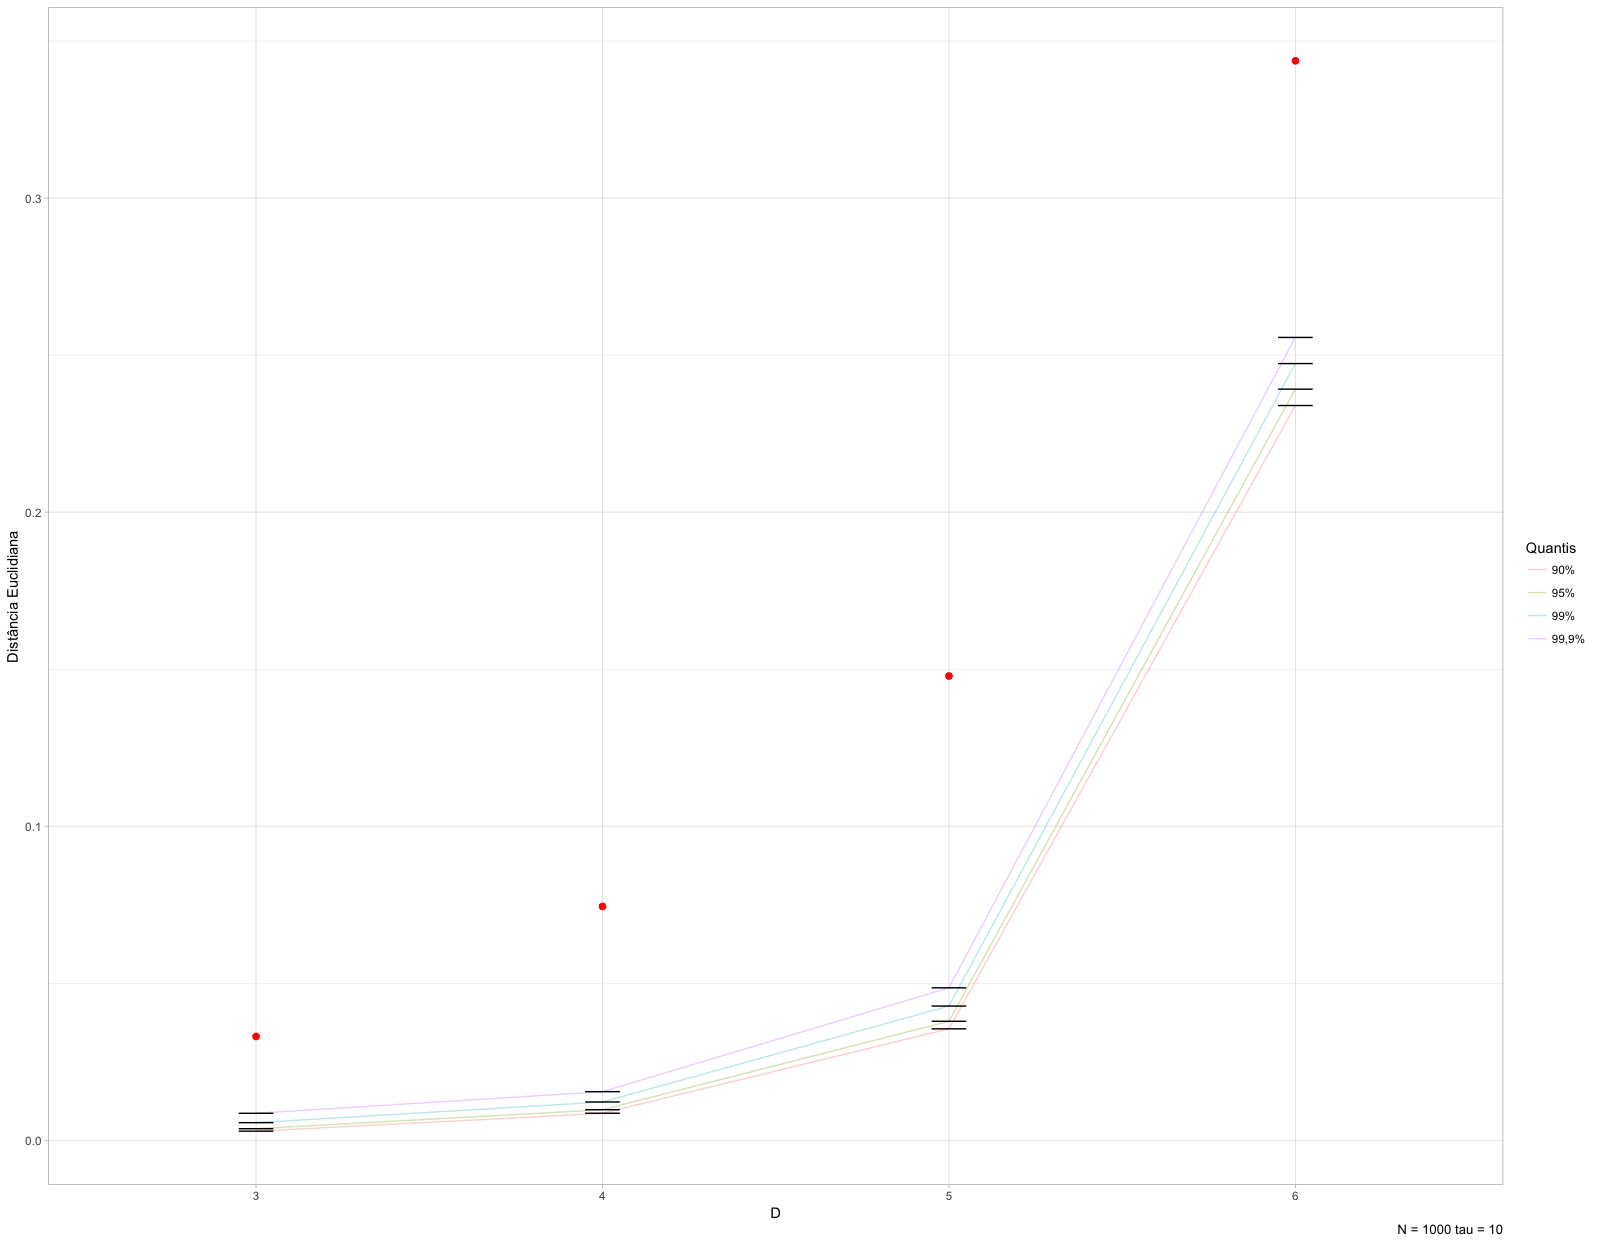
\includegraphics[width=1\linewidth]{ConfidInt_nao_estacionaria_1k_t10}
	\caption{Pontos característicos das séries não estacionárias e intervalos de confiança.}\label{Fig:ConfidInt_nao_estacionaria_1k_t10}
\end{figure}

A aplicação do teste à sequência obtida pelo método de séries estacionárias pode ser observada na figura~\ref{Fig:ConfidInt_estacionaria_1k_t10}.
Novamente, o teste leva à rejeição da sequência pois para qualquer $D= 3, 4, 5, 6$ os descritores produzem pontos a distâncias euclidianas maiores do que as estipuladas pelos intervalos de confiança estabelecidos. 
O código~\ref{code:Estacionaria} foi utilizado para gerar a sequência; ver apêndice~\ref{codigo}.

\begin{figure}
	\centering
	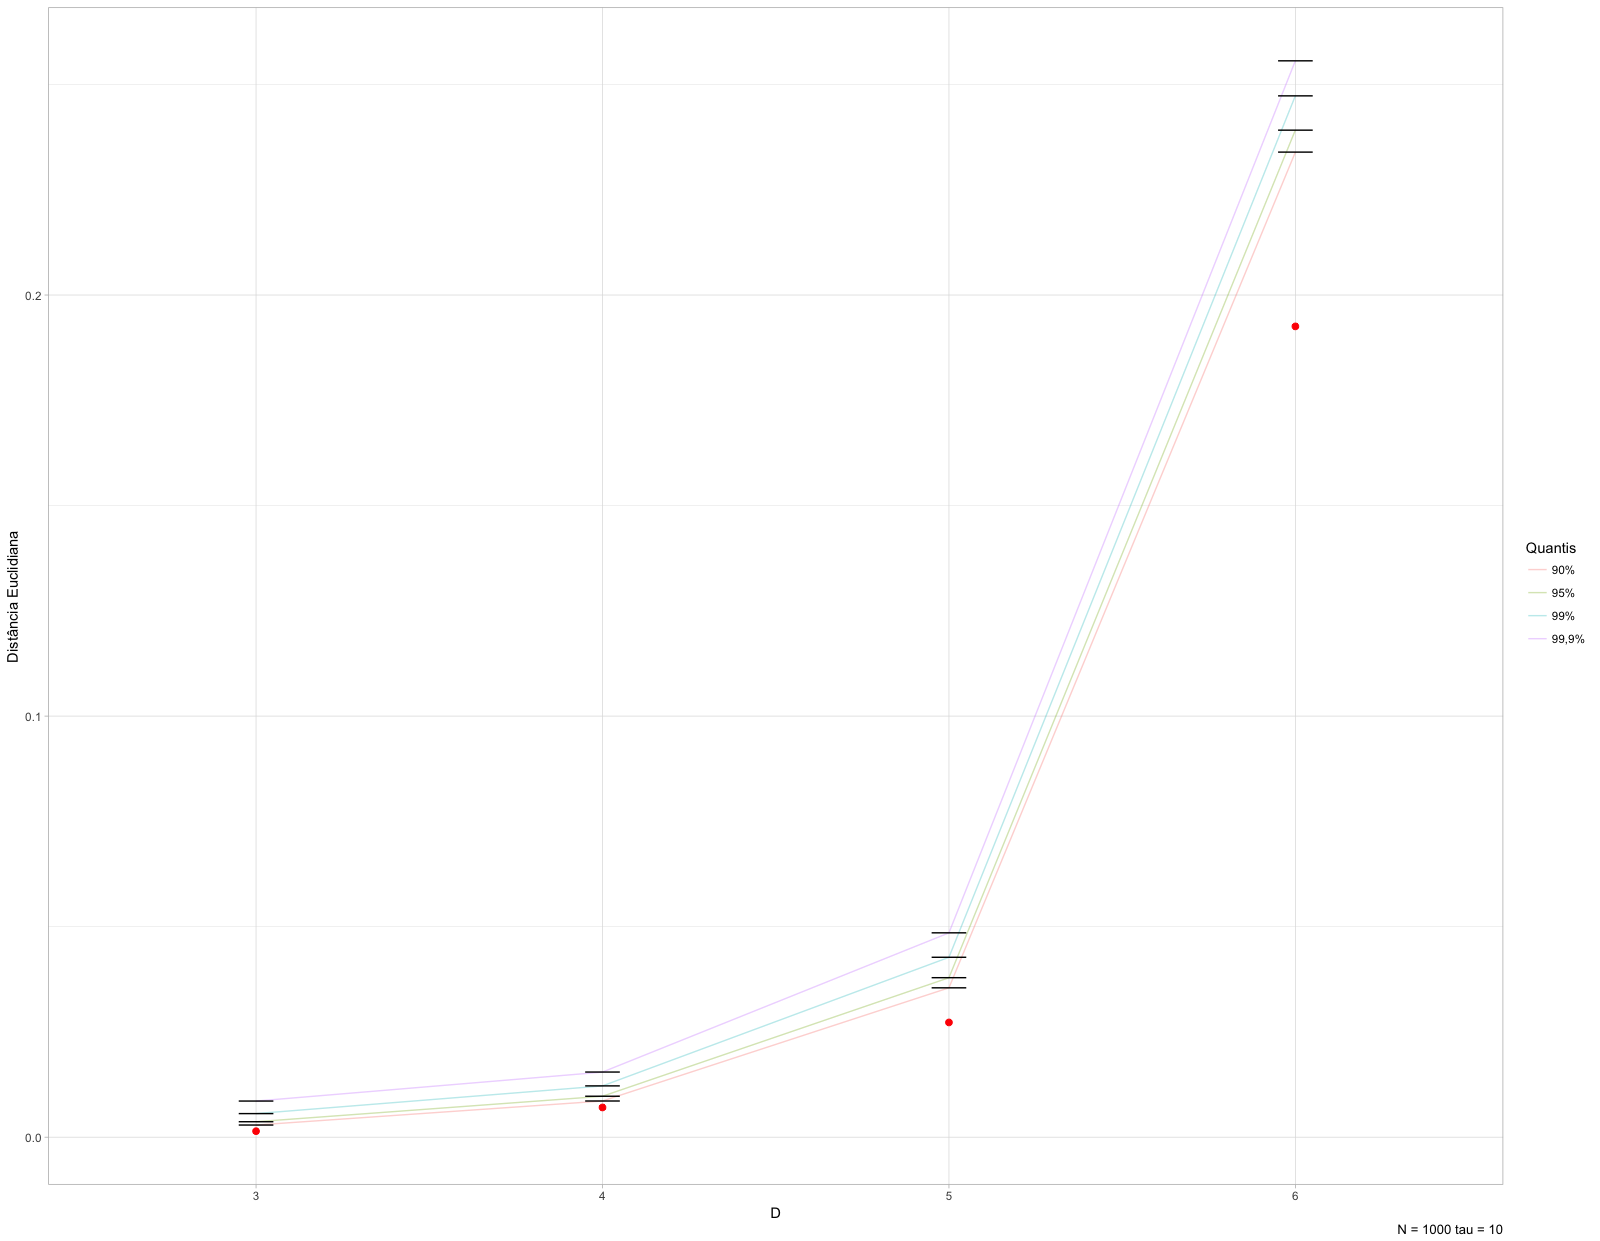
\includegraphics[width=1\linewidth]{ConfidInt_estacionaria_1k_t10}
	\caption{Pontos característicos das séries estacionárias e intervalos de confiança.}\label{Fig:ConfidInt_estacionaria_1k_t10}
\end{figure}

A seguir analisamos uma série determinística com comportamento caótico: o mapa logístico.
O mapa logístico é a sequência obtida pela recursão
\begin{equation}
x_{n+1} = r x_n(1-x_n),
\end{equation}
com $0<x_1<1$ e $0<r\leq 4$.
Utilizamos $r=4$, $x_0=0.01$.
Iteramos o mapa \num{10000} vezes para alcançar estabilidade, e só coletamos a partir de $n=10001$.

A aplicação do teste à sequência obtida pelo
mapa logístico pode ser observada na figura~\ref{Fig:ConfidInt_mapa_logistico_1k_t1}.
Mais uma vez, o teste leva à rejeição da sequência pois para qualquer $D= 3, 4, 5, 6$ os descritores produzem pontos a distâncias euclidianas maiores do que as estipuladas pelos intervalos de confiança estabelecidos. 
O código~\ref{code:MapaLogistico} foi utilizado para gerar a sequência; ver apêndice~\ref{codigo}.

Convém notar que o mapa logístico já foi usado como fonte de dados pseudoaleatórios, e este resultado mostra que ele não é adequado (com os parâmetros aqui escolhidos) para esse propósito.

\begin{figure}
	\centering
	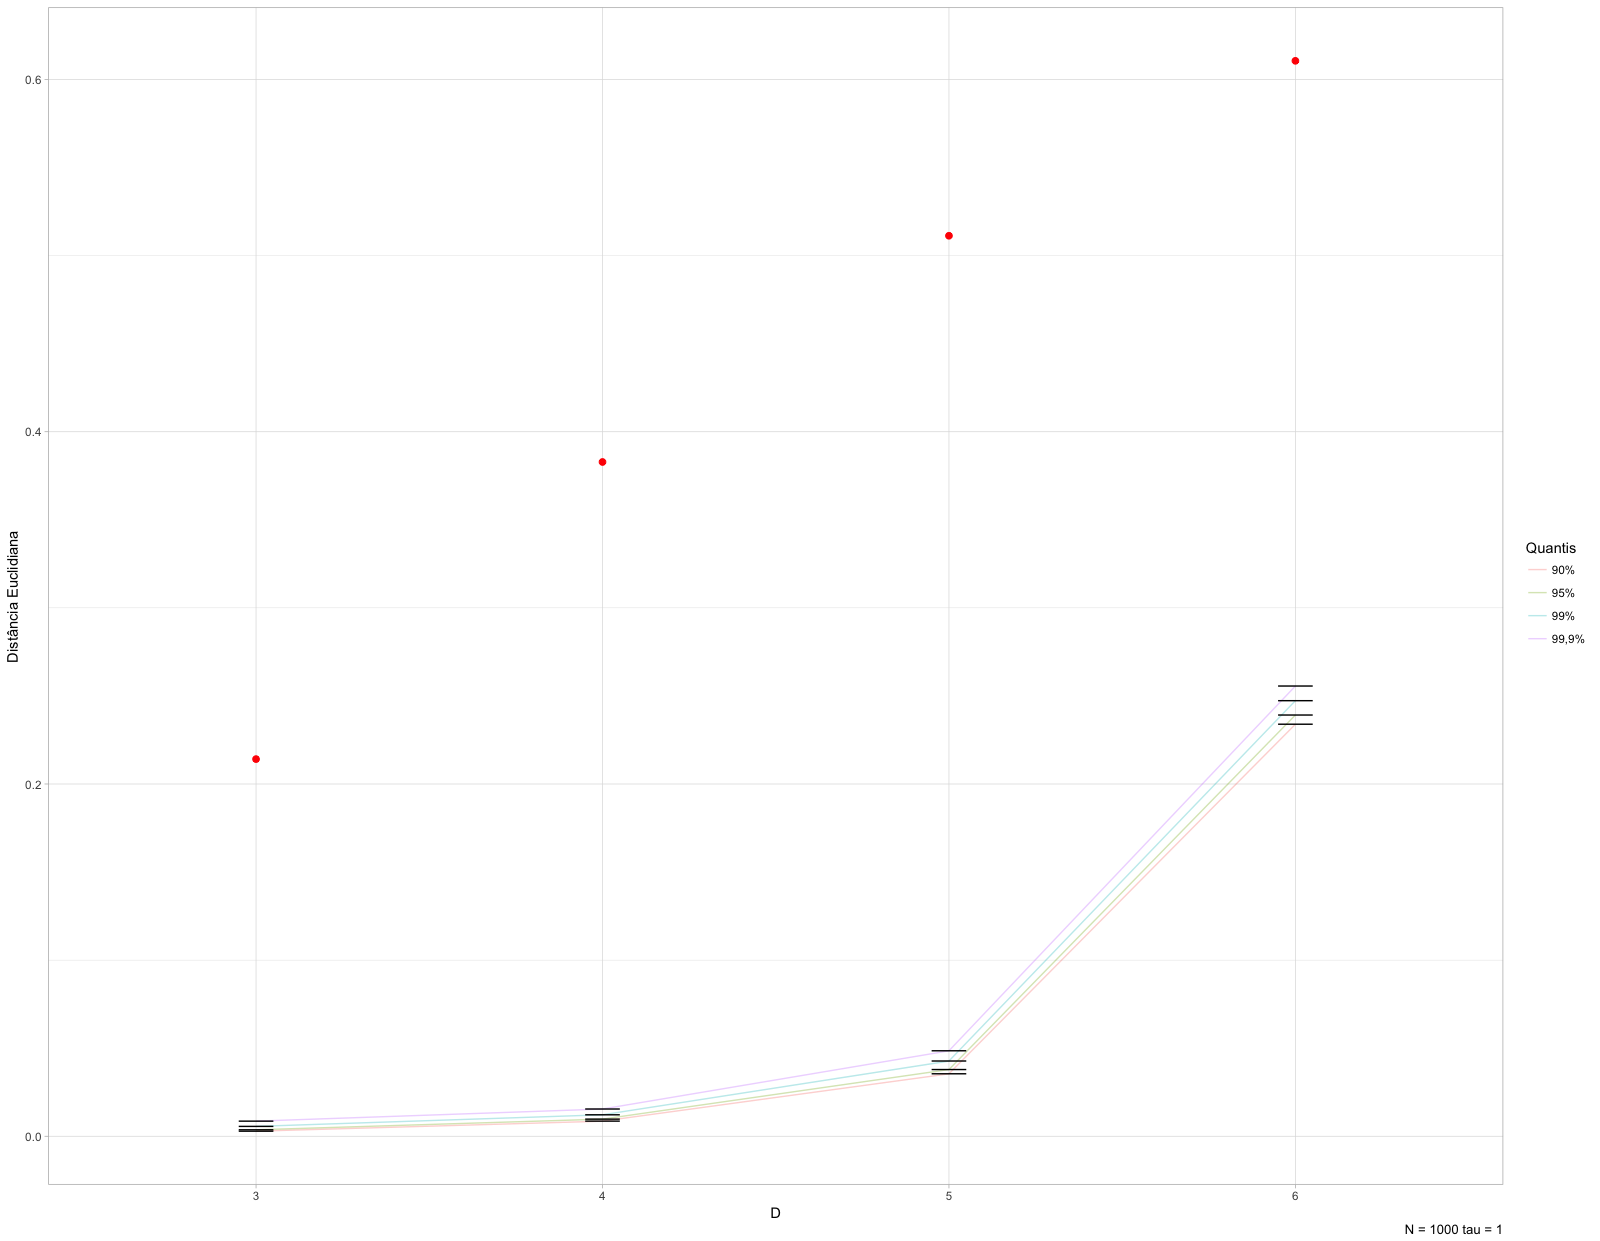
\includegraphics[width=1\linewidth]{ConfidInt_mapa_logistico_1k_t1}
	\caption{Pontos característicos do mapa logístico e intervalos de confiança.}\label{Fig:ConfidInt_mapa_logistico_1k_t1}
\end{figure}

Poder do teste
Seja T um teste estatístico com região crítica C para avaliarmos hipóteses a respeito do parâmetro $\theta$. A função poder do teste é a probabilidade de rejeitarmos H0 dado o valor de $\theta$. Neste caso, temos que
\begin{equation}
\pi(\theta) = P[rejeitar H_0|\theta] = P[T \in C|\theta]
\end{equation}


Aqui analizamos 

\begin{figure}
	\centering
	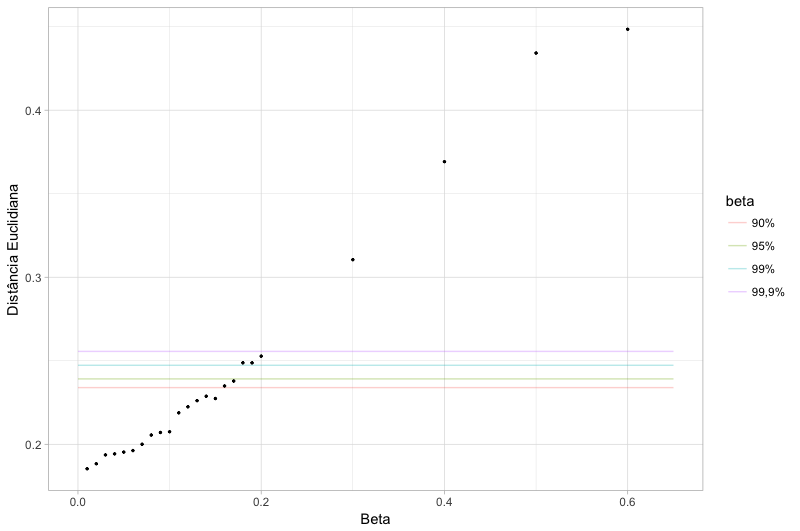
\includegraphics[width=1\linewidth]{beta_1k_D6_t1}
	\caption{Poder do teste.}\label{Fig:beta}
\end{figure}
